\subsection{Towards robust boosted jet tagging}
\label{sec:searchII:intro}
When we first studied W-tagging at 13 \TeV in context with the analysis of the 2015 dataset, Section~\ref{sec:searchI:wtagging}, two interesting correlations were observed:

\bigskip
1) A strong dependence of the AK8 CHS softdrop ($\beta = 0$) jet mass on jet \PT and

2) a strong dependence of the AK8 CHS $\tau_{21}$ cut efficiency on pileup.
\bigskip

The reason we studied the softdrop algorithm as an alternative to pruning in 2015 was, besides the possibility it would result in a higher signal efficiency, that we knew it had certain favorable qualities compared to other groomers: Softdrop removes all sensitivity to the soft divergences of QCD, by removing all soft emission, more specifically the non-global logarithmic terms (NGLs) in the jet mass~\cite{Dasgupta:2013ihk}. These arise from constellations where, for instance, a soft gluon is radiated into the jet cone, as illustrated in Figure~\ref{fig:searchII:ngls}. 
\begin{figure}[h!]
\centering
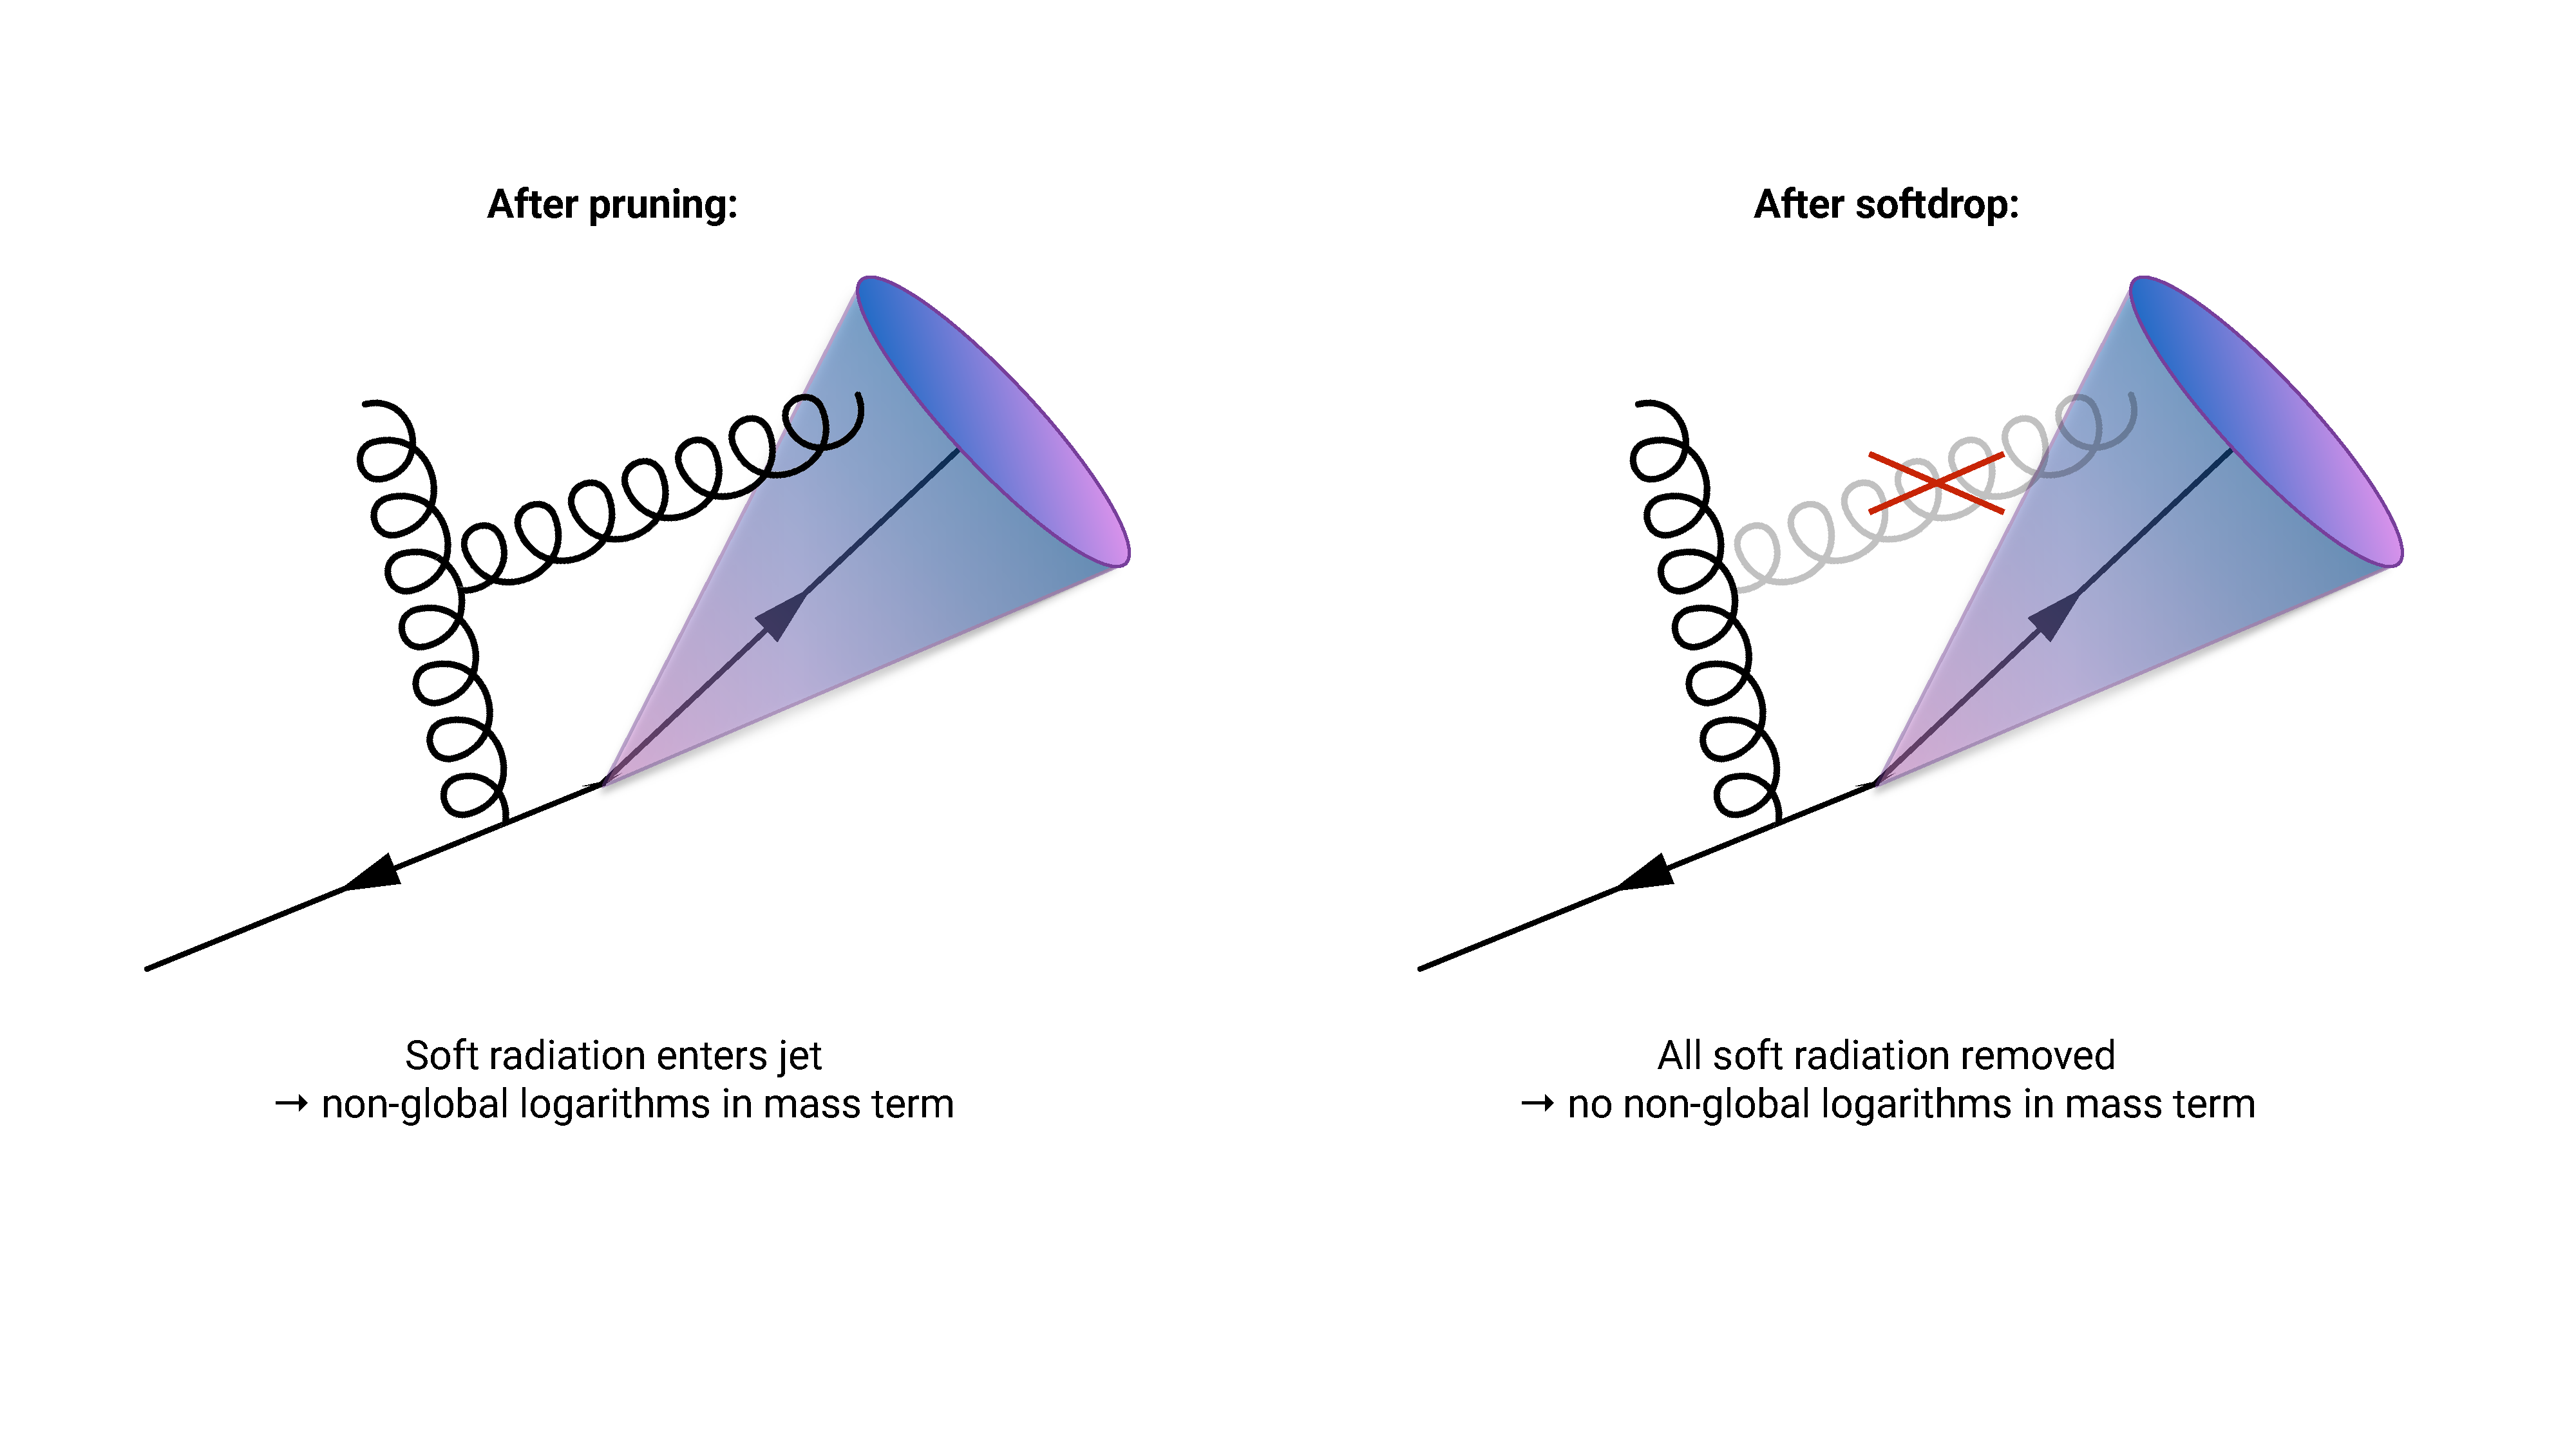
\includegraphics[width=0.69\textwidth]{figures/analysis/search2/misc/ngls.pdf}
\caption{The pruning algorithm does not remove all soft emission and therefore has non-global logarithmic terms in the jet mass. Softdrop ($\beta = 0$) completely removes soft emissions and is therefore free of non-global logarithms.}
\label{fig:searchII:ngls}
\end{figure}
The consequence of this is that you can calculate the softdrop jet mass to way higher precision than what is possible for other grooming algorithms or for the plain jet mass (NGLs are the main reason a full resummation of the plain jet mass beyond NLL (considering e.g multiple-emission effects) accuracy does not exist). Despite this not being a precision measurement analysis, we had theoretically well-motivated reasons for wanting the baseline CMS V-tagger to be softdrop-based. However, despite being less sensitive to soft radiation for QCD jets, signal jets groomed with softdrop were found to be far more sensitive to the underlying event than pruned jets~\cite{Dasgupta:2015yua}. Figure~\ref{fig:searchII:ue} shows the signal efficiency for pruning (left) and softdrop (right) as a function of jet transverse momenta when including FSR only, FSR+ISR, hadronization and hadronization + underlying event.
\begin{figure}[h!]
\centering
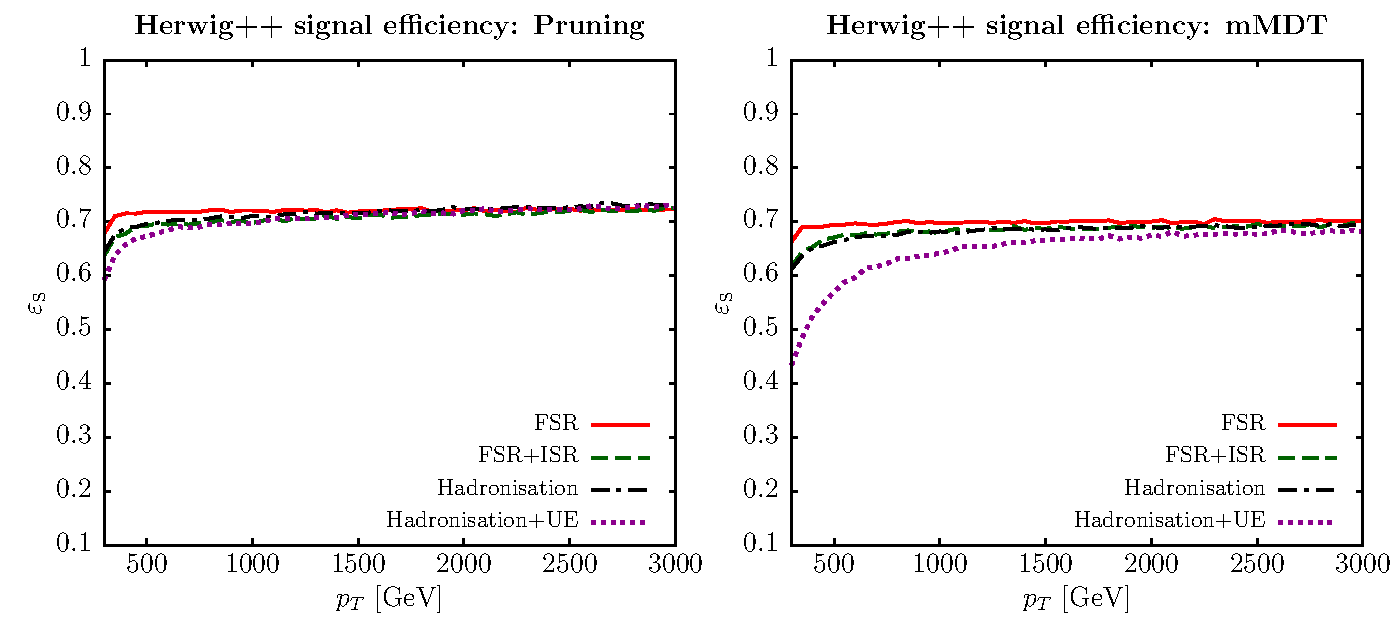
\includegraphics[width=0.79\textwidth]{figures/analysis/search2/misc/pruningvssd_ue.pdf}
\caption{The signal efficiency for pruning (left) and softdrop (right) as a function of jet \PT when adding FSR, ISR, hadronization and UE. THe UE has a severe impact on the softdrop efficiency for signal jets~\cite{Dasgupta:2015yua}. }
\label{fig:searchII:ue}
\end{figure}
On parton level, as well as after hadronization, the two algorithms perform very similar as a function of \PT. However, once UE contamination is added, the softdrop tagging efficiency is severely affected. This can be explained by the larger effective radius considered by the softdrop algorithm ( $\propto \mV/\PT \sqrt{z_{cut}(1-z_{cut})}$ ) in comparison to pruning ( $\propto \mV/\PT$ ). This observation corresponds very well with the shift in jet mass we observed for softdrop as a function of \PT in Section~\ref{sec:searchI:wtagging}: As the jet \PT decreases the softdrop effective radius increases and the jet mass mean shifts to higher values, due to absorbing more background radiation. If softdrop would be our new default tagger, a better rejection of pileup and UE contamination would be needed. In parallel to the ongoing theoretical work on groomers, a novel pileup removal algorithm had been proposed: Pileup per particle identification (PUPPI)~\cite{Bertolini2014}. Described in detail in Section~\ref{subsub:objreco:puppi}, PUPPI considers not only charged pileup but rather reweights each particle in the jet with its probability of arising from pileup. PUPPI had proven it self far superior to the current CHS algorithm in terms of jet observables for large radius jets, and therefore seemed like the obvious choice to address both issues listed above: The sensitivity of softdrop regarding UE contamination and the strong pileup dependence of $\tau_{21}$. The focus of Search II would therefore be on the commissioning of a novel W-tagger. There are interesting changes and inclusions in the analysis strategy as well: The inclusion of a $\PZpr \rightarrow \WW$ signal hypothesis and the addition of a completely new analysis, the single V-tag analysis.

\subsection{Analysis strategy}
The analysis strategy for this search is conceptually the same as for Search I. In addition, we'll take advantage of the n-subjettiness categorization and do an additional analysis in parallel: A search for excited quark resonances $\rm{q^*}$~\cite{Bauer1987,PhysRevD.42.815} decaying to qW or qZ.
We call this the single V-tag analysis, and the analysis selection only differs in that one jet is not required to pass the V-tag selection (groomed mass and n-subjettiness). The \VV analysis is hereby referred to as the double V-tag analysis. The difference between the two analyses is illustrated in Figure~\ref{fig:searchII:svsd}. 
\begin{figure}[h!]
\centering
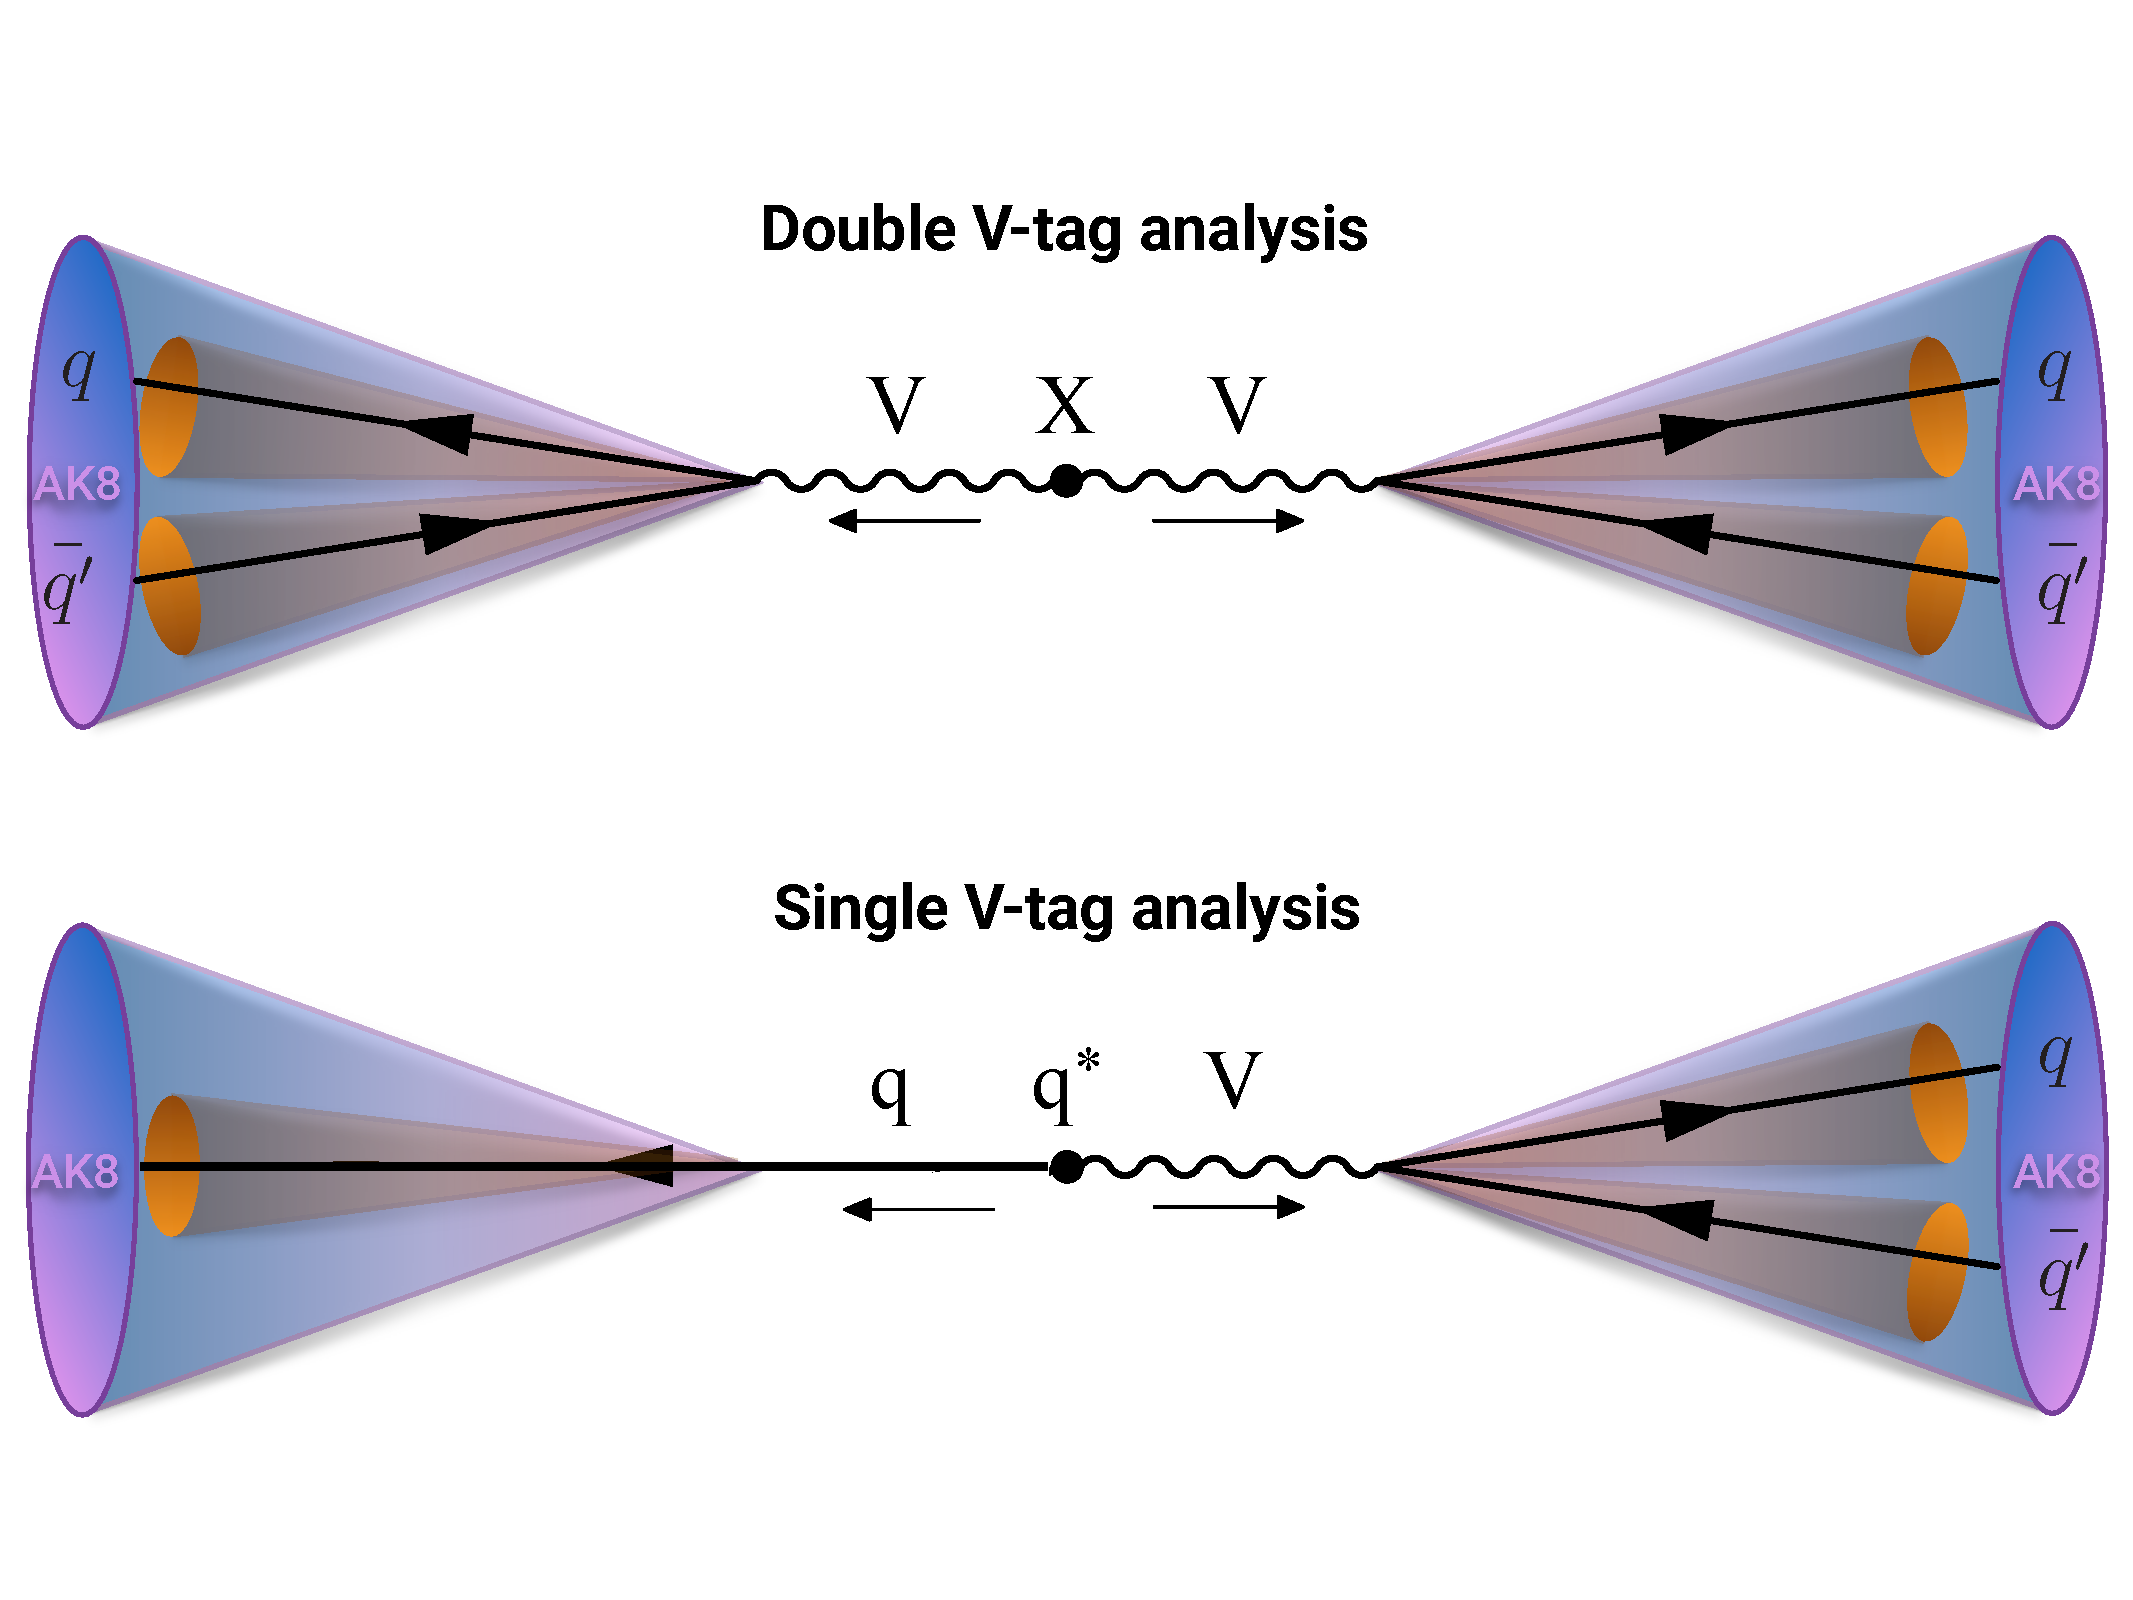
\includegraphics[height=6.5cm]{figures/analysis/search2/misc/singlevsdoubletag.pdf}
\caption{The double (top) and single (bottom) W/Z-tag analysis.}
\label{fig:searchII:svsd}
\end{figure}
In addition, limits are set on a $\PZpr \rightarrow \WW$ signal hypothesis in the double V-tag analysis, another 13 \TeV first.\newline
This analysis was published in two steps: An early Physics Analysis Summary (PAS) based on 12.9 \fbinv of 2016 data~\cite{CMS-PAS-B2G-16-021}, describing the new  PUPPI+softdrop based V-tagger as well as the single V-tag analysis, and a second analysis topping up with the full 2016 data~\cite{PhysRevD.97.072006}. The commissioning of the new \PW\PZ-tagger has also been documented in a jet performance Physics Analysis Summary~\cite{CMS-PAS-JME-16-003}. As the new V-tagger was developed and commissioned in the context of the early analysis, which was also were the single V-tag analysis was first published with 13 \TeV data, the main emphasis will be on the work presented in CMS-PAS-B2G-16-021~\cite{CMS-PAS-B2G-16-021}. The second part of the results chapter, Section~\ref{sec:searchII:brg17001res}, includes the results obtained using the full 2016 dataset of 35.9 \fbinv.

\subsection{Data and simulated samples}
\label{sec:searchII:samples}
As mentioned above, the analysis of the 2016 dataset was done in two steps: One analysis based on 12.9 \fbinv of early 2016 data, describing the new W-tagger and single V-tag category, and a second paper topping up with the full 2016 dataset, corresponding to 35.9 \fbinv.\par
The \BulkG and HVT signal samples are modeled in precisely the same way as in 2015. For the single V-tag $\textrm{q}^*$ samples, we simulate unpolarized boson with a compositeness scale $\Lambda$ set equal to the resonance mass. These are generated to leading order using \PYTHIA version 8.212~\cite{Sjostrand:2007gs}. \par
The background Standard Model processes; QCD, W+jets and Z+jets are all simulated to leading order. V+jets is simulated with \amcatnlo~\cite{Alwall:2014hca,Alwall:2007fs}, while three different combinations of matrix element and shower generators is used for QCD as these predictions are known to differ: \PYTHIA only, the leading order mode of \amcatnlo{} matched with \PYTHIA, and \HERWIG{++}~2.7.1~\cite{Bahr:2008pv} with tune CUETHS1~\cite{Khachatryan:2015pea}.

\subsection{Event selection}
\subsubsection{Triggering}
The triggers used in this analysis are the same ones as in 2015 (see Section~\ref{sec:searchI:trigger}), however, due to the new single V-tag analysis, the trigger turn-ons have this time been re-evaluated separately requiring either one or two jets to have an offline softdrop jet mass above 65 \GeV.
\par Figure~\ref{fig:searchII:trigger-fits} shows the trigger turn-on curves as a function of dijet invariant mass for jets passing one of the three inclusive triggers only, one of the grooming triggers only and when combining all of them. The turn-on curves are shown for all jet pairs passing loose selections as described in Section \ref{sec:searchI:preselection}. Zero, one or two of the two jets is further required to have a softdrop mass larger than 65 GeV.

\begin{figure}[h!]
\centering
% 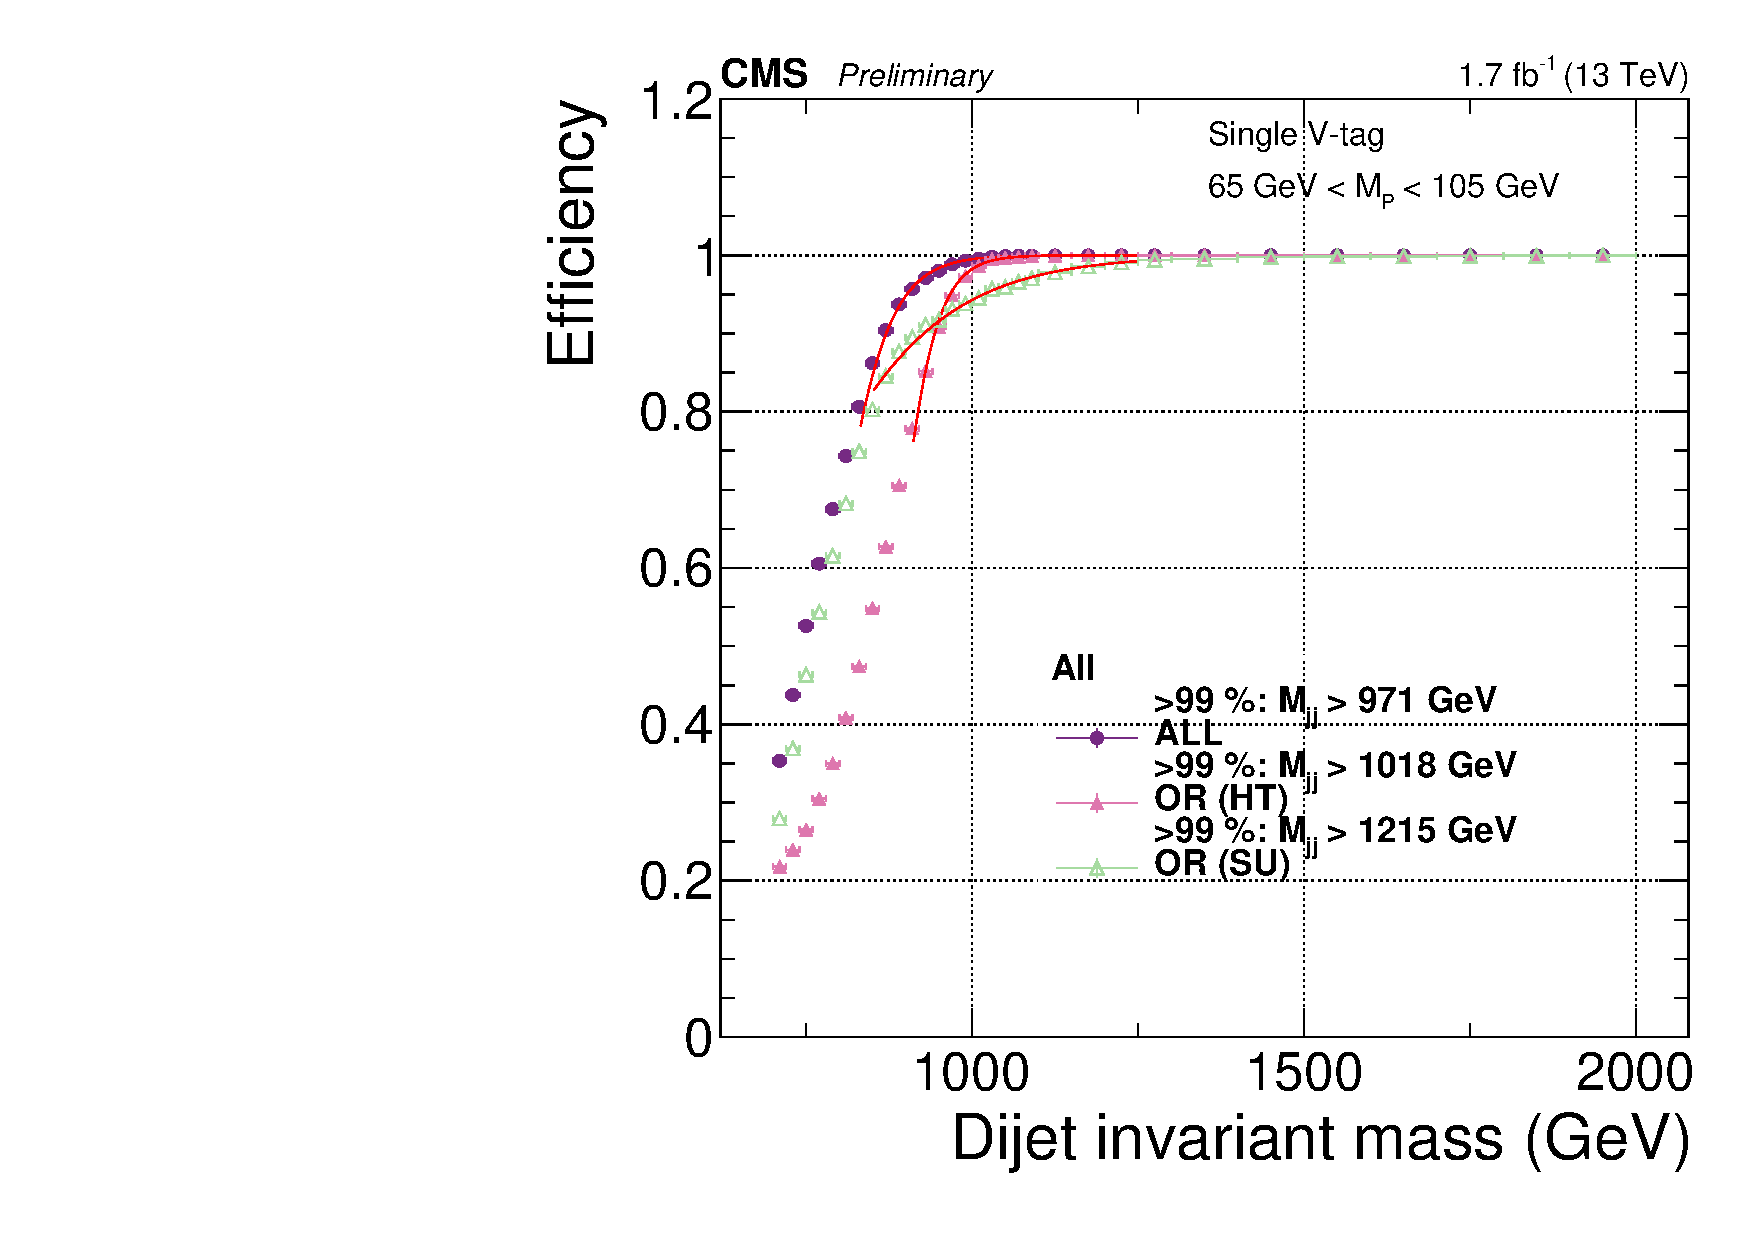
\includegraphics[width=0.4\textwidth]{figures/analysis/search2/AN-16-398/plots/trigger/triggereffMjj-ALL_SingleTag_runAll.pdf}
% 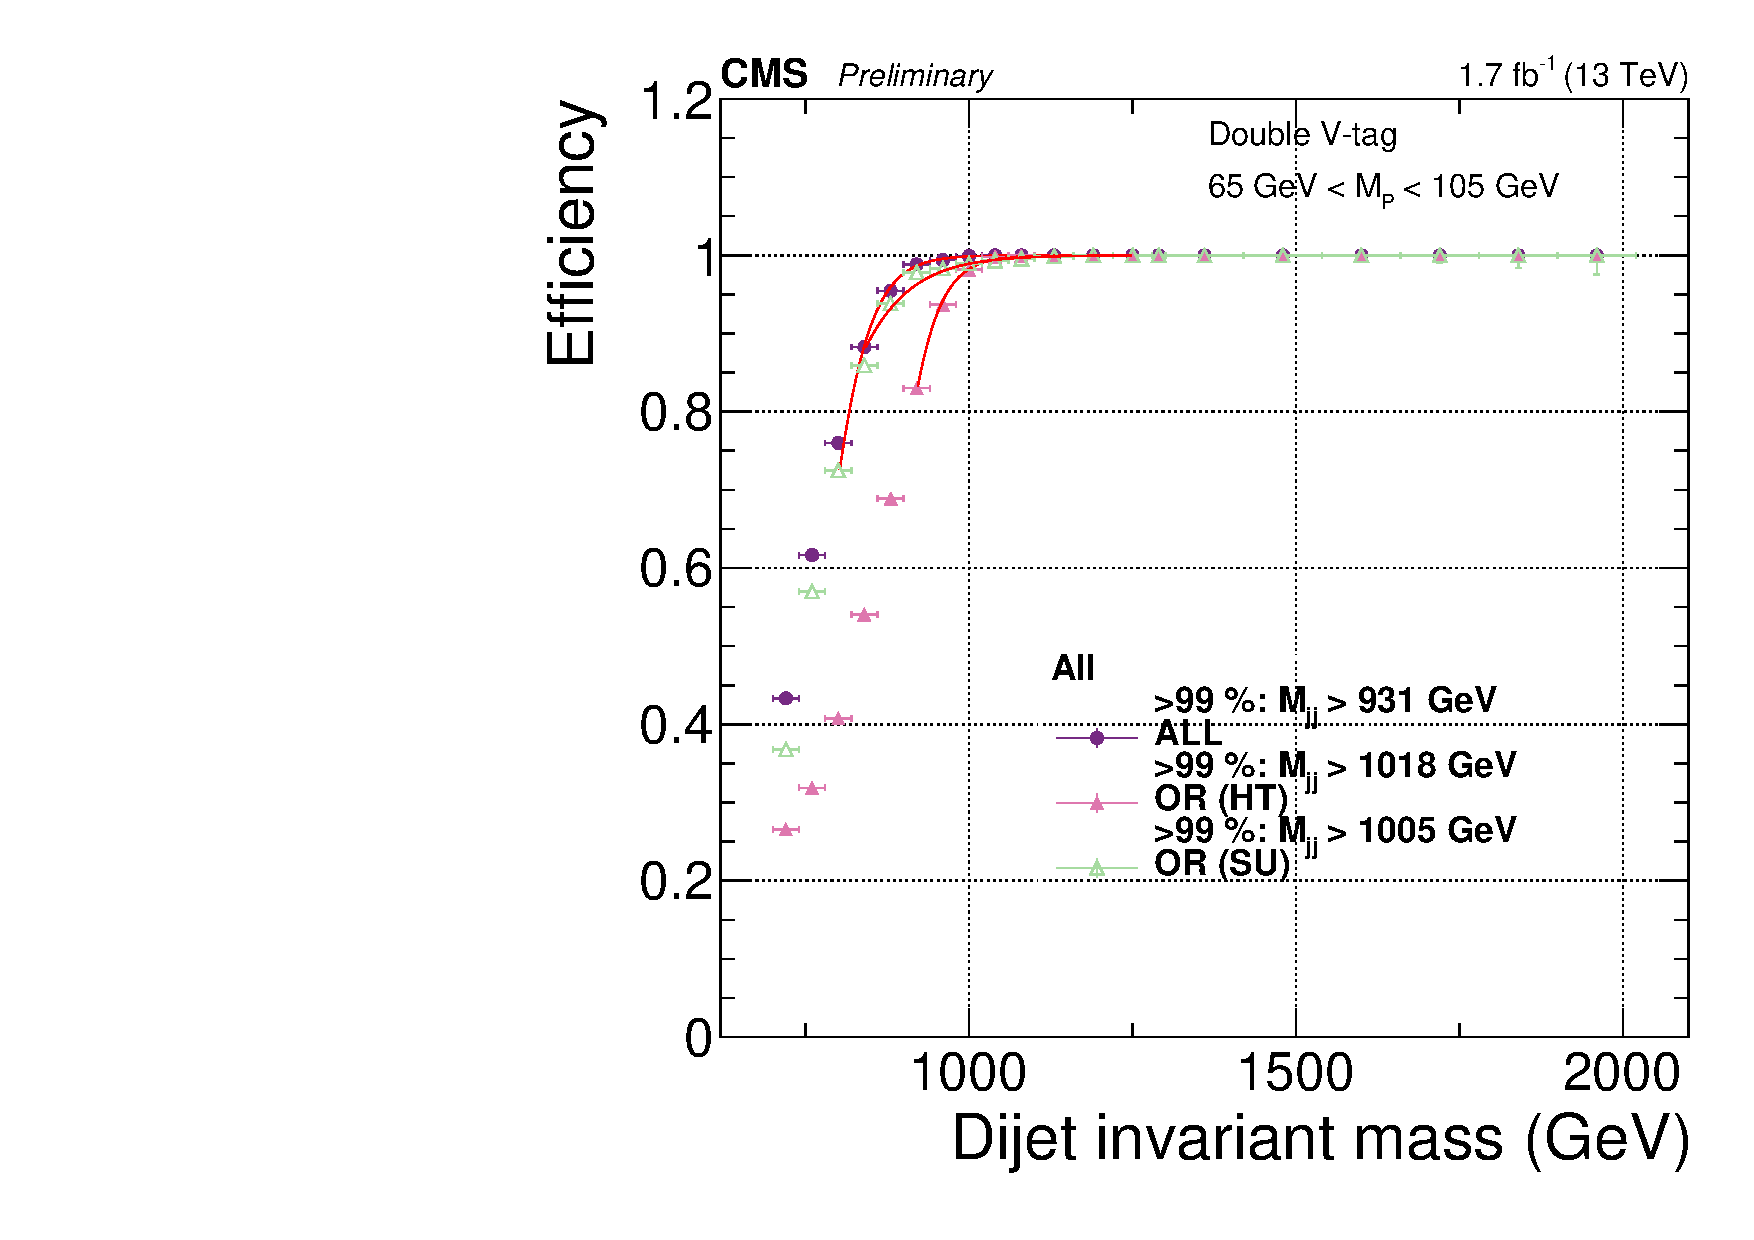
\includegraphics[width=0.4\textwidth]{figures/analysis/search2/AN-16-398/plots/trigger/triggereffMjj-ALL_DoubleTag_runAll.pdf}
% 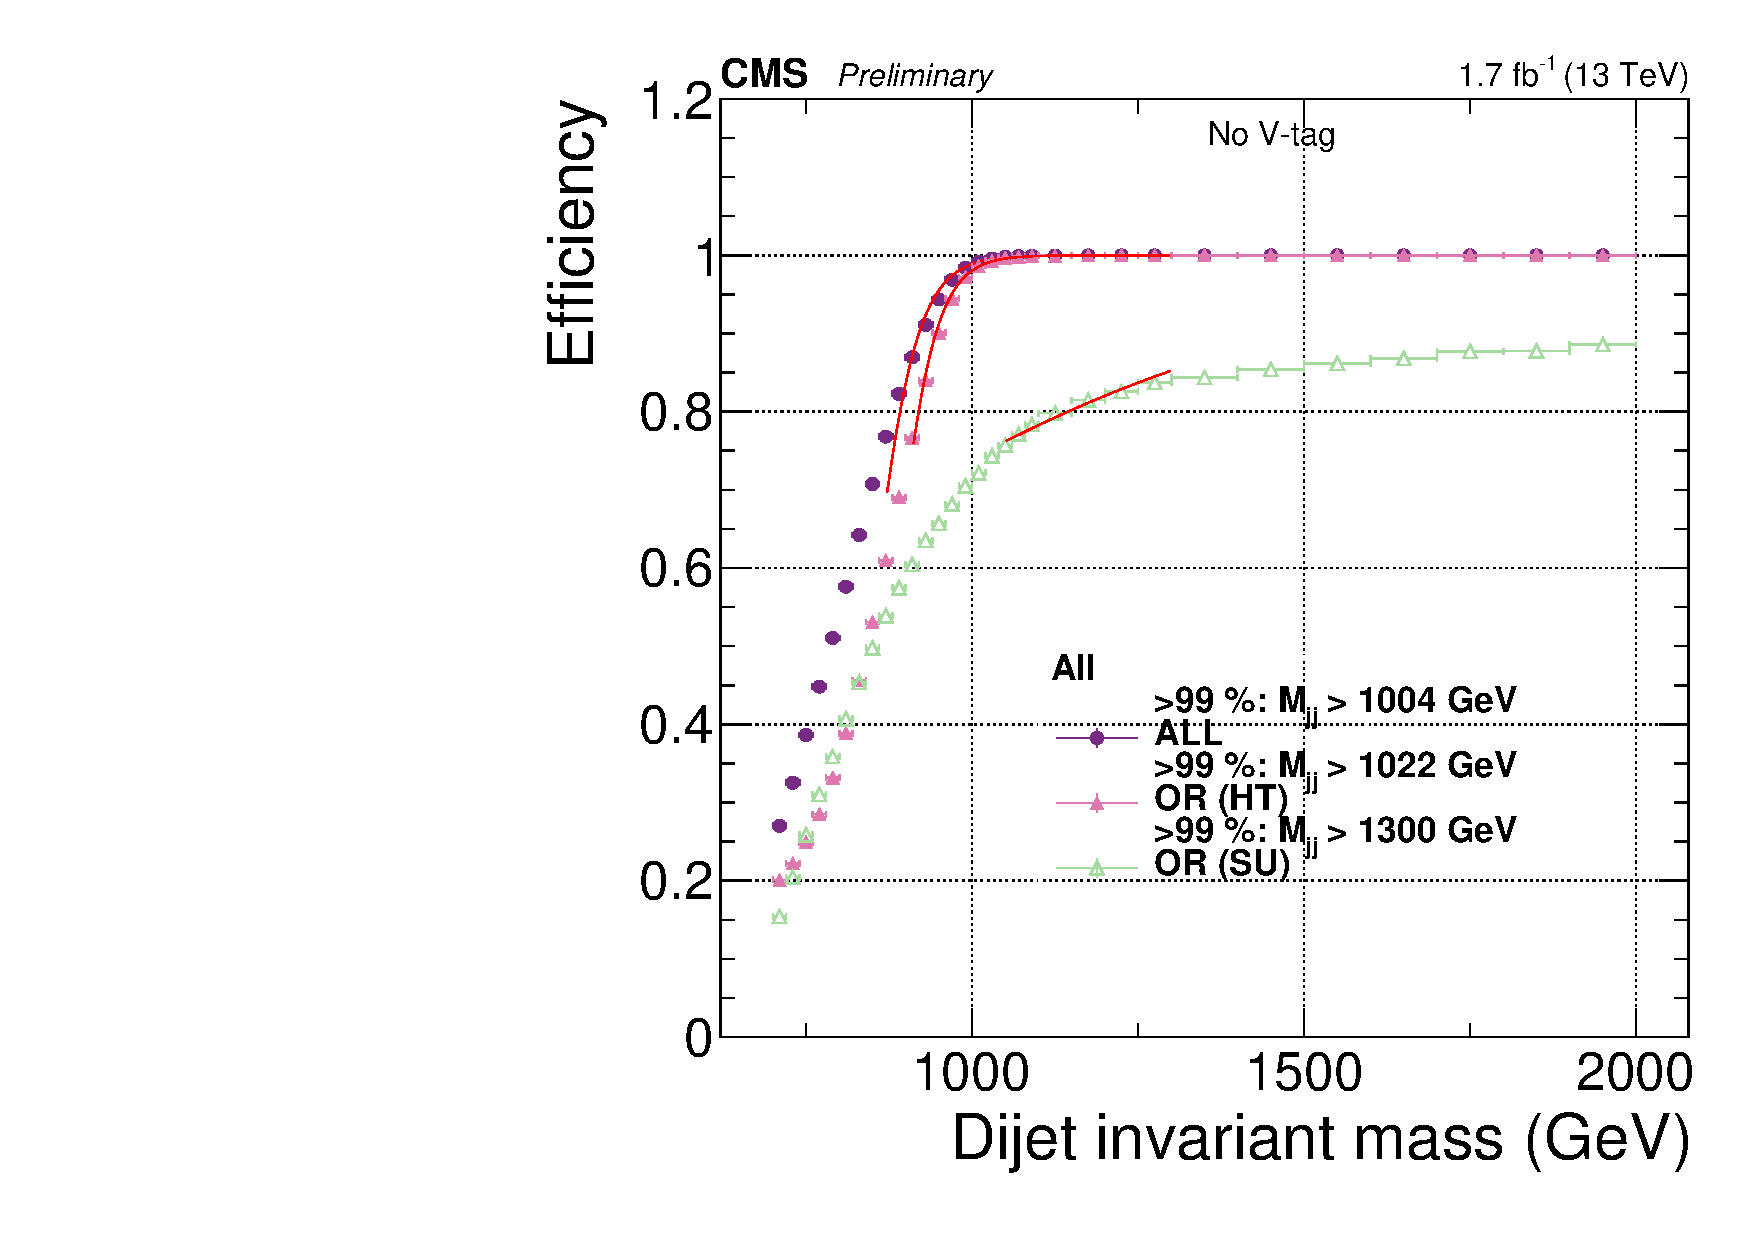
\includegraphics[width=0.4\textwidth]{figures/analysis/search2/AN-16-398/plots/trigger/triggereffMjj-ALL_noTag_runAll.pdf}
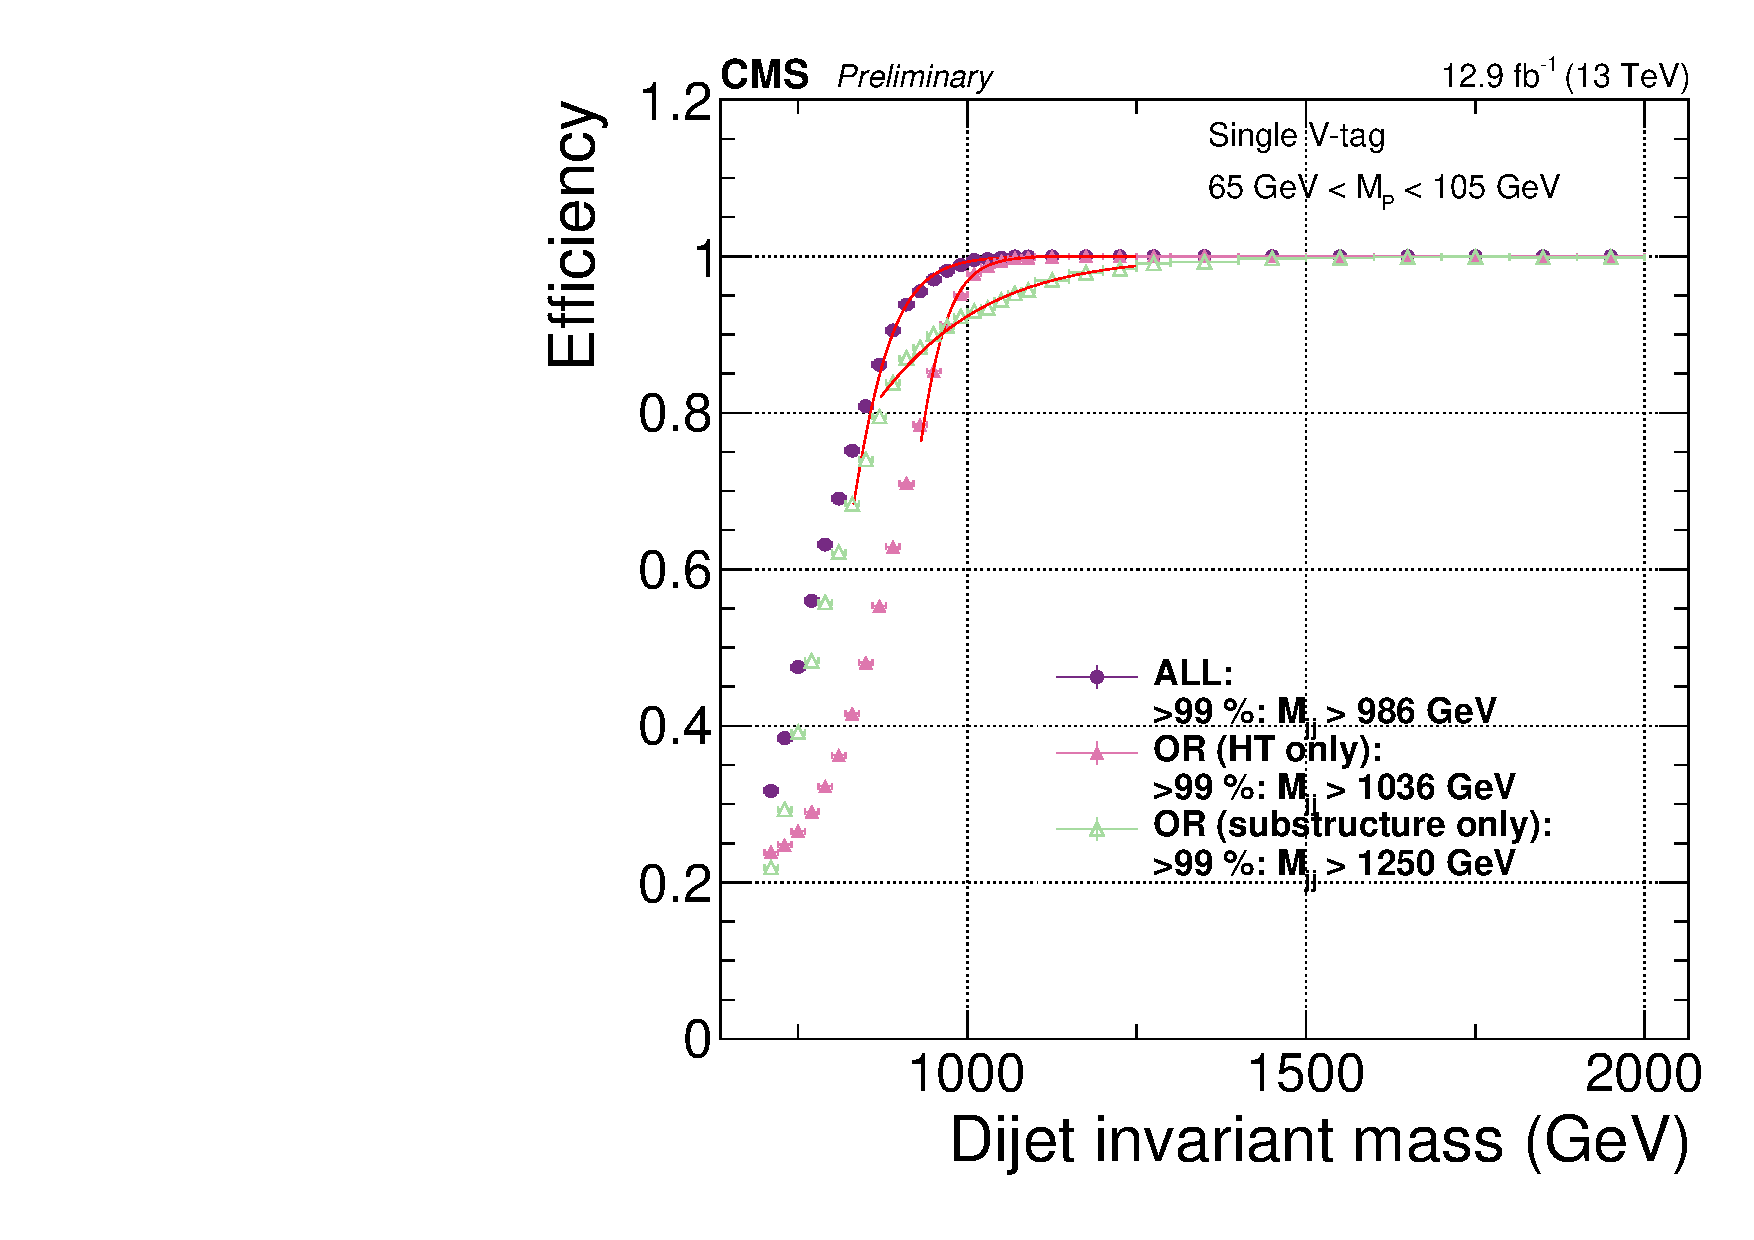
\includegraphics[width=0.49\textwidth]{figures/analysis/search2/AN-16-235/plots/triggereffMjj-ALL_SingleTag.pdf}
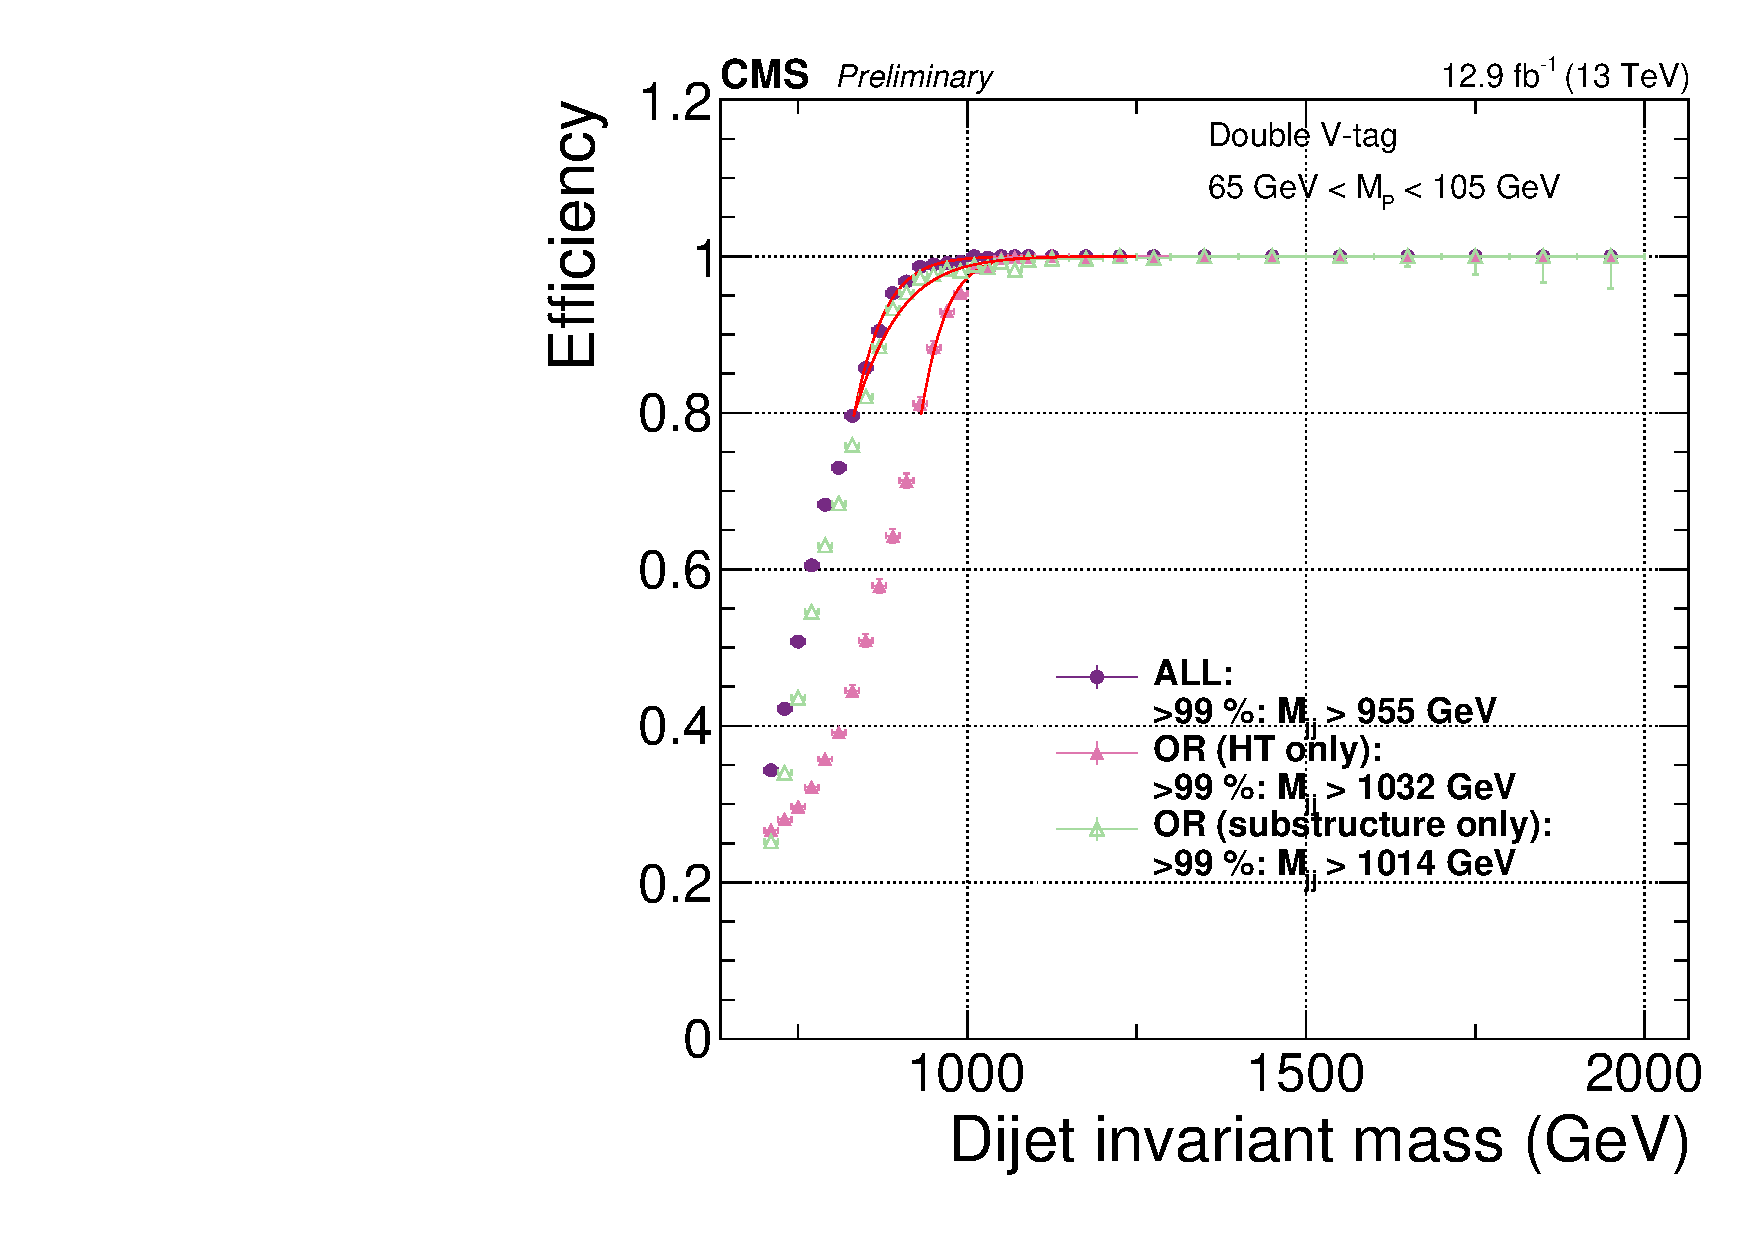
\includegraphics[width=0.49\textwidth]{figures/analysis/search2/AN-16-235/plots/triggereffMjj-ALL_DoubleTag.pdf}\\
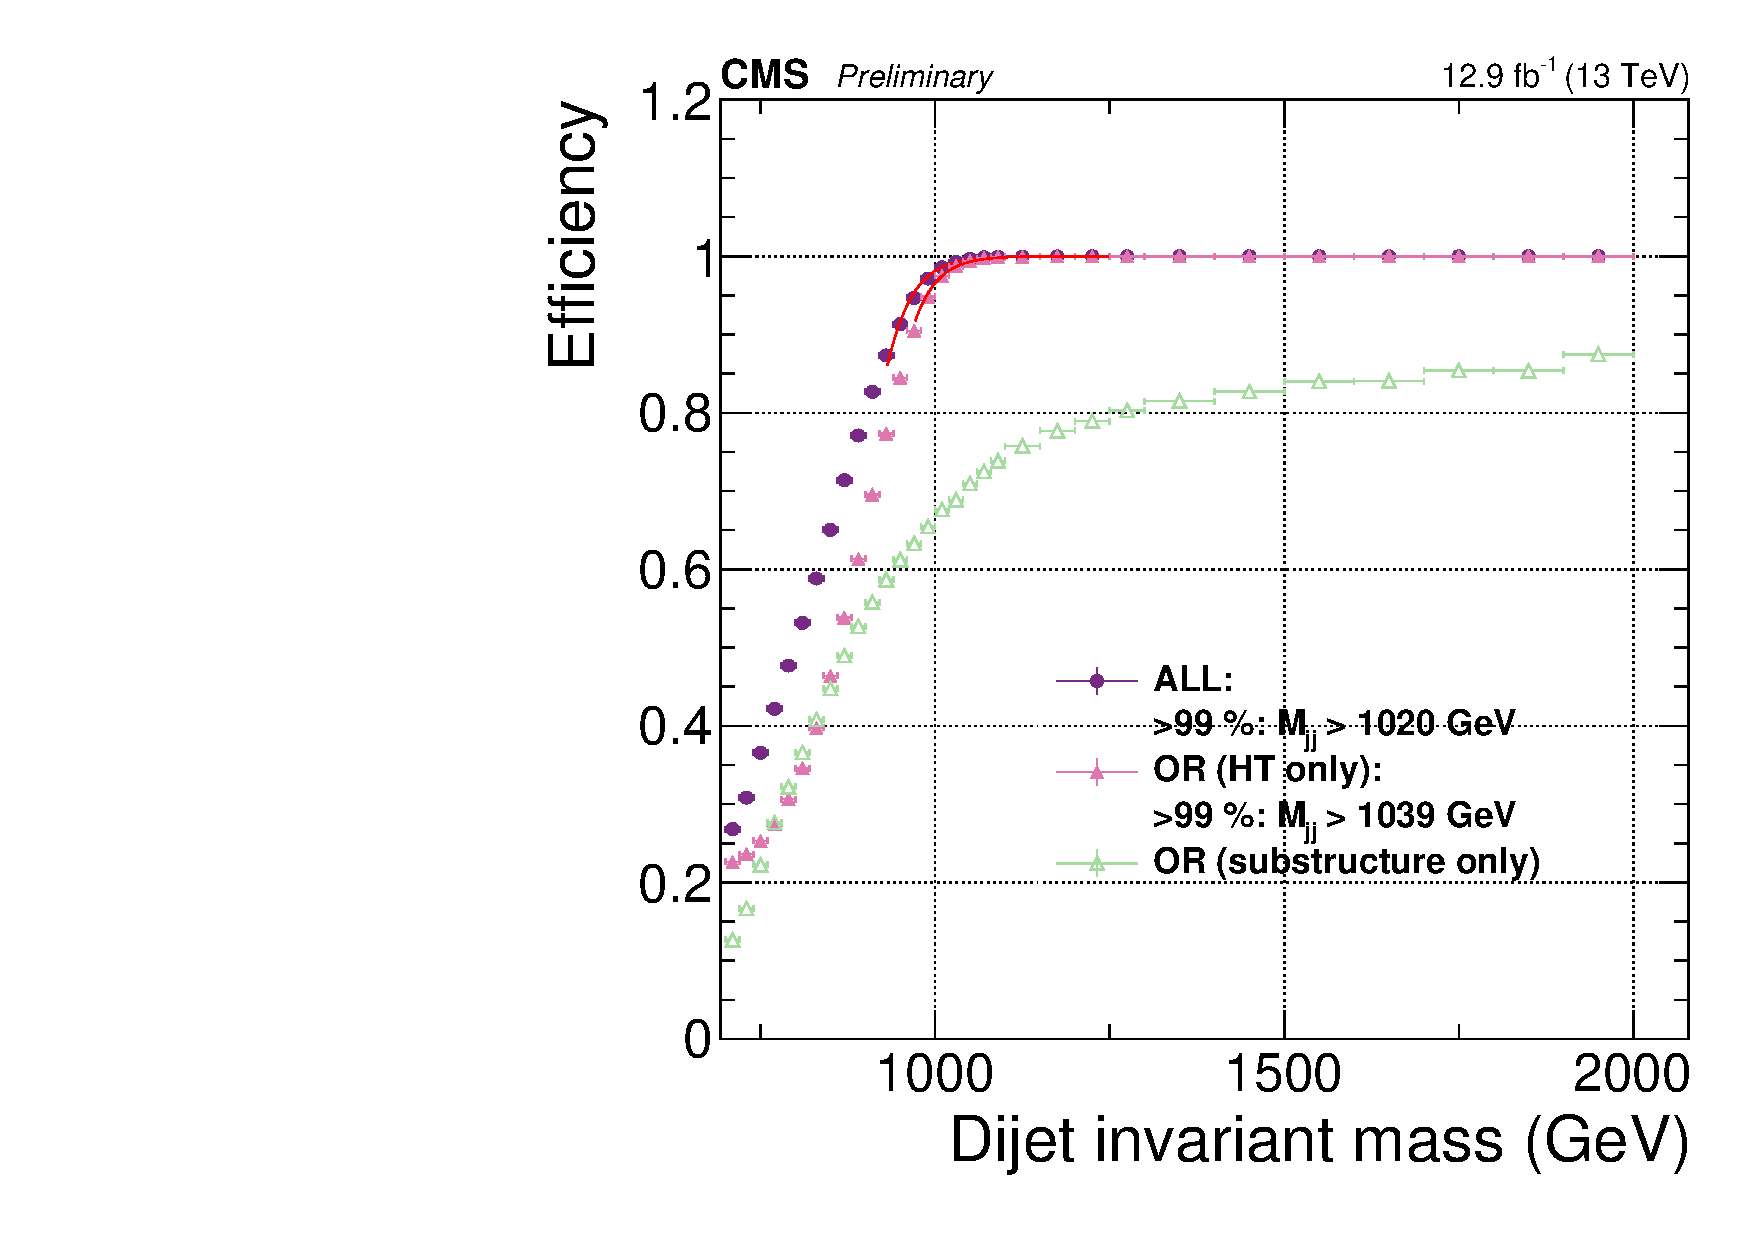
\includegraphics[width=0.49\textwidth]{figures/analysis/search2/AN-16-235/plots/triggereffMjj-ALL_noTag.pdf}
\caption{Comparison of trigger efficiencies for jets passing one of the HT-triggers only (pink), for jets passing one of the grooming-triggers only (green) and for jets passing one of the HT-triggers or one of the grooming triggers (purple). Here as a function of dijet invariant mass for all jet pairs passing loose selections and where one jet has a softdrop mass larger than 65 GeV (top left), both jets have a softdrop mass larger than 65 GeV (top right) and where no mass cut is applied (bottom). }
\label{fig:searchII:trigger-fits}
\end{figure}
Including grooming triggers lowers the 99\% trigger efficiency threshold by around 50(80) \GeV in the single (double) tag category once substructure is requested on the analysis level. Using the or of all triggers, we are safely on the trigger plateau for dijet invariant masses above 955(986) \GeV in the double (single) tag category, setting the analysis threshold at a dijet invariant mass of 955 \GeV for the double tag analysis and 990 \GeV for the single tag analysis. For controlplots, where no groomed mass window is applied, a trigger threshold of 1020 GeV is used.
\par Trigger efficiencies as a function of the offline softdrop-jet mass for the \\ 
\texttt{HLT\_AK8PFJet360\_TrimMass30} trigger are shown in Figure~\ref{fig:searchII:grooming-mj-trigger}. Here the jet transverse momentum of one of the jets is required to be at least 600 GeV and no other mass cut is applied. This trigger requires one jet to have a trimmed mass above 30 GeV at HLT level and reaches the trigger plateau for groomed-jet masses around 50 GeV. As reference trigger, the prescaled trigger \texttt{HLT\_PFJet320} is used. 
\begin{figure}[htb]
\centering
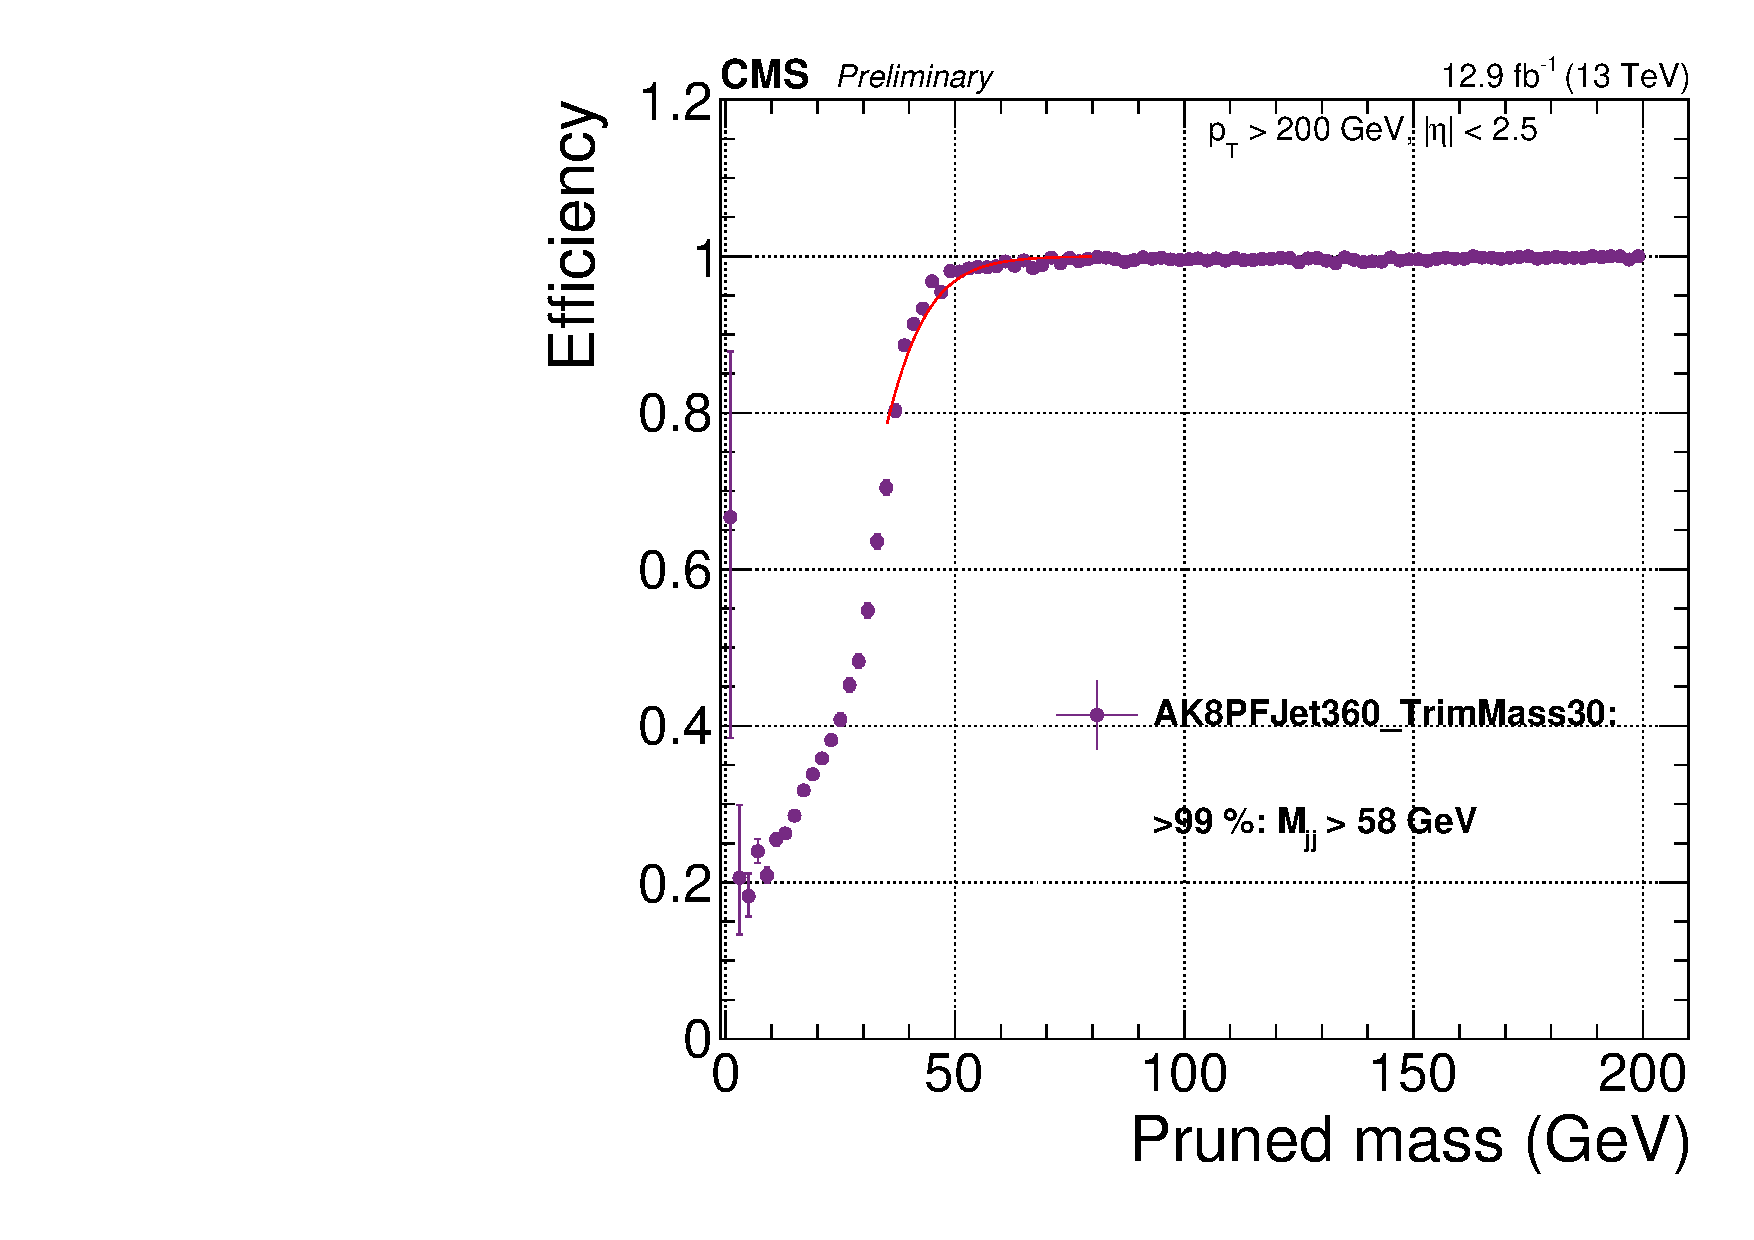
\includegraphics[width=0.49\textwidth]{figures/analysis/search2/AN-16-235/plots/triggereff-prunedmass_fit.pdf}
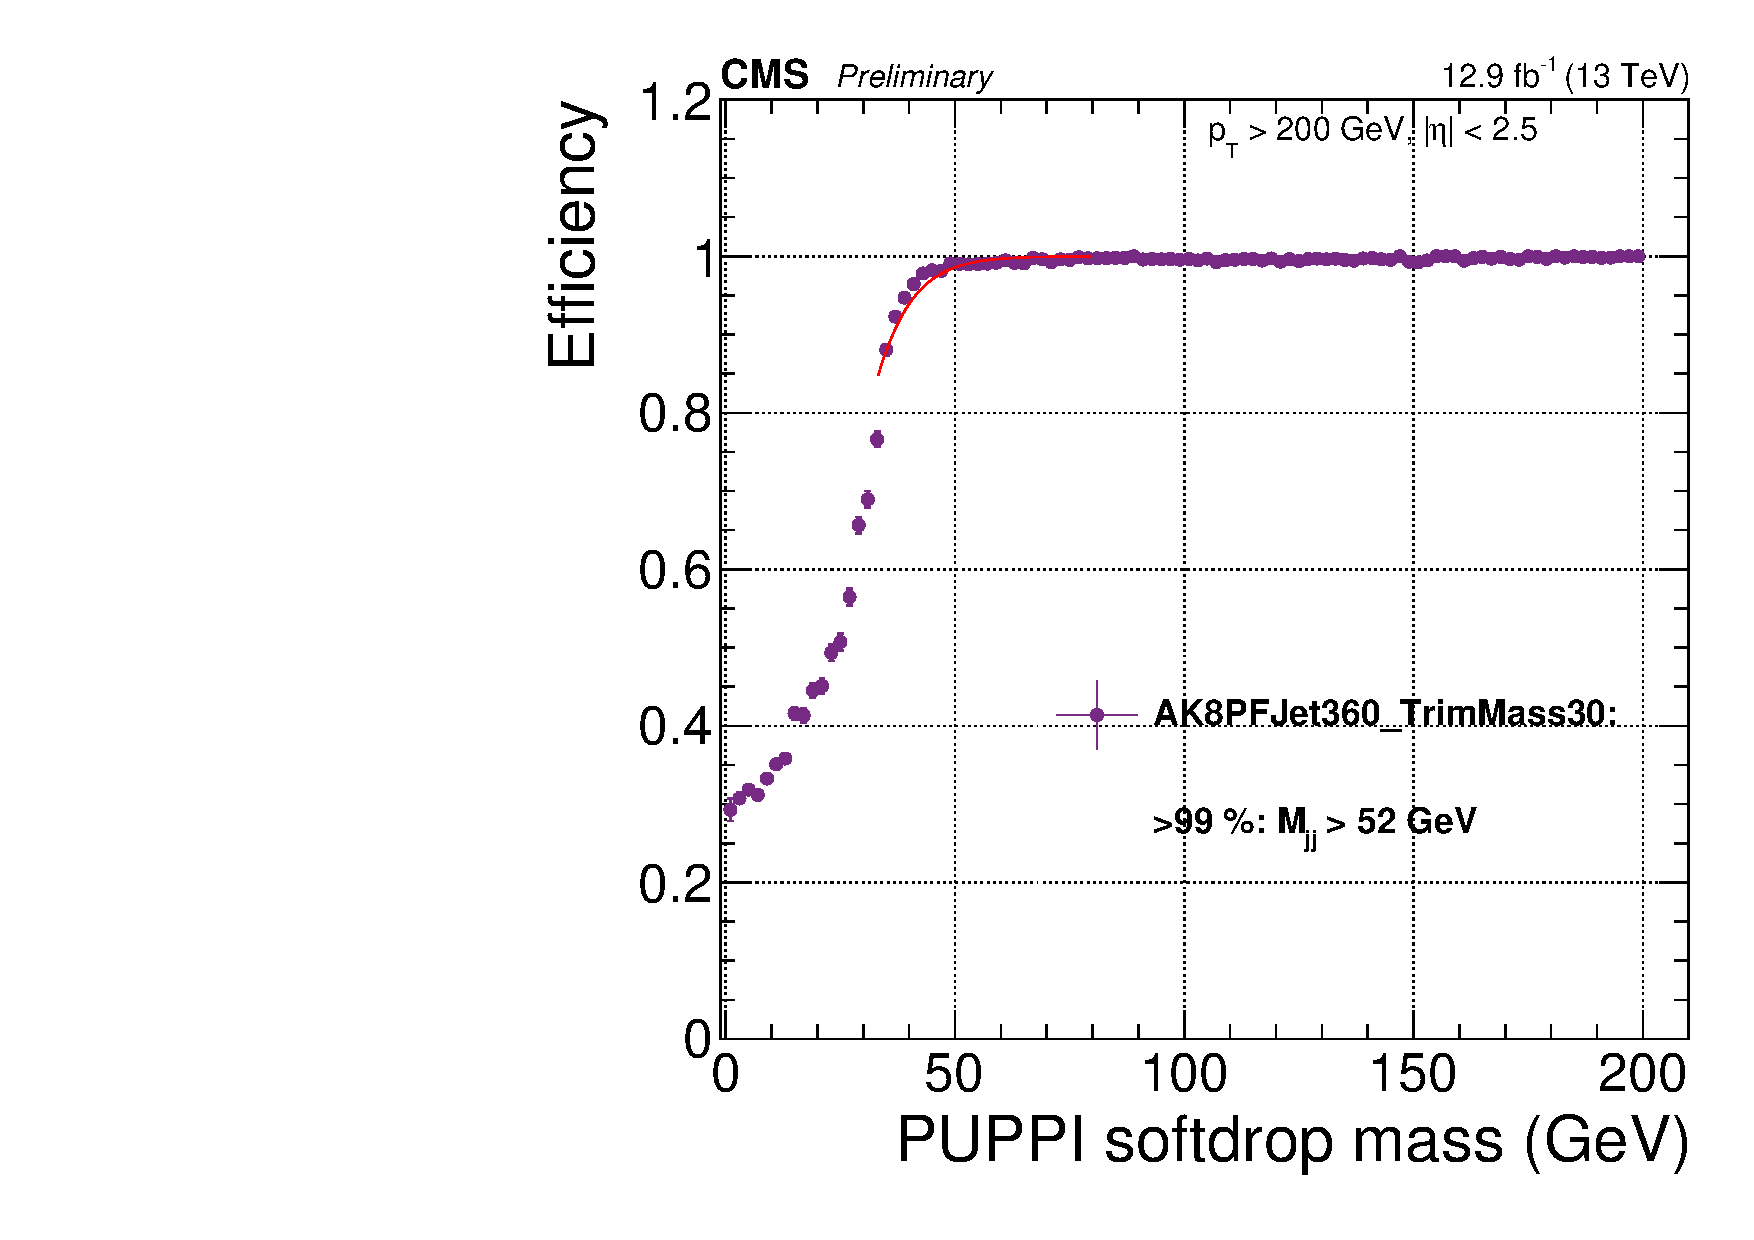
\includegraphics[width=0.49\textwidth]{figures/analysis/search2/AN-16-235/plots/triggereff-sdmass_fit.pdf}
\caption{Efficiency for the \texttt{HLT\_AK8PFJet360\_TrimMass30} trigger as a function of pruned-jet (left) and softdrop-jet (right) mass for jets with $\PT > \unit{600}{\GeV}$.}
\label{fig:searchII:grooming-mj-trigger}
\end{figure}

\subsubsection{Preselection}
The same preselections as in Search I, described in \label{sec:search1:preselection}, have been applied: We require two AK R=0.8 jets with CHS applied pre-clustering, required to pass the tight jet ID requirement, $\PT>200 \GeV$ and $|\eta|<2.5$. The same QCD t-channel suppressing cut of $|\Delta \eta|<1.3$ is required together with the following trigger thresholds on the dijet invariant mass: $\mjj > \unit{955} {\GeV}$ for the double V-tag and $\unit{990} {\GeV}$ for the single V-tag analysis. The jet \PT (top left), $\eta$ (top right), $\Delta \eta_{jj}$ and dijet invariant mass (bottom left) for the two leading jets in the event after loose preselections are applied is shown in Figure~\ref{fig:searchII:kinematics-all}.
\begin{figure}[h!]
\centering
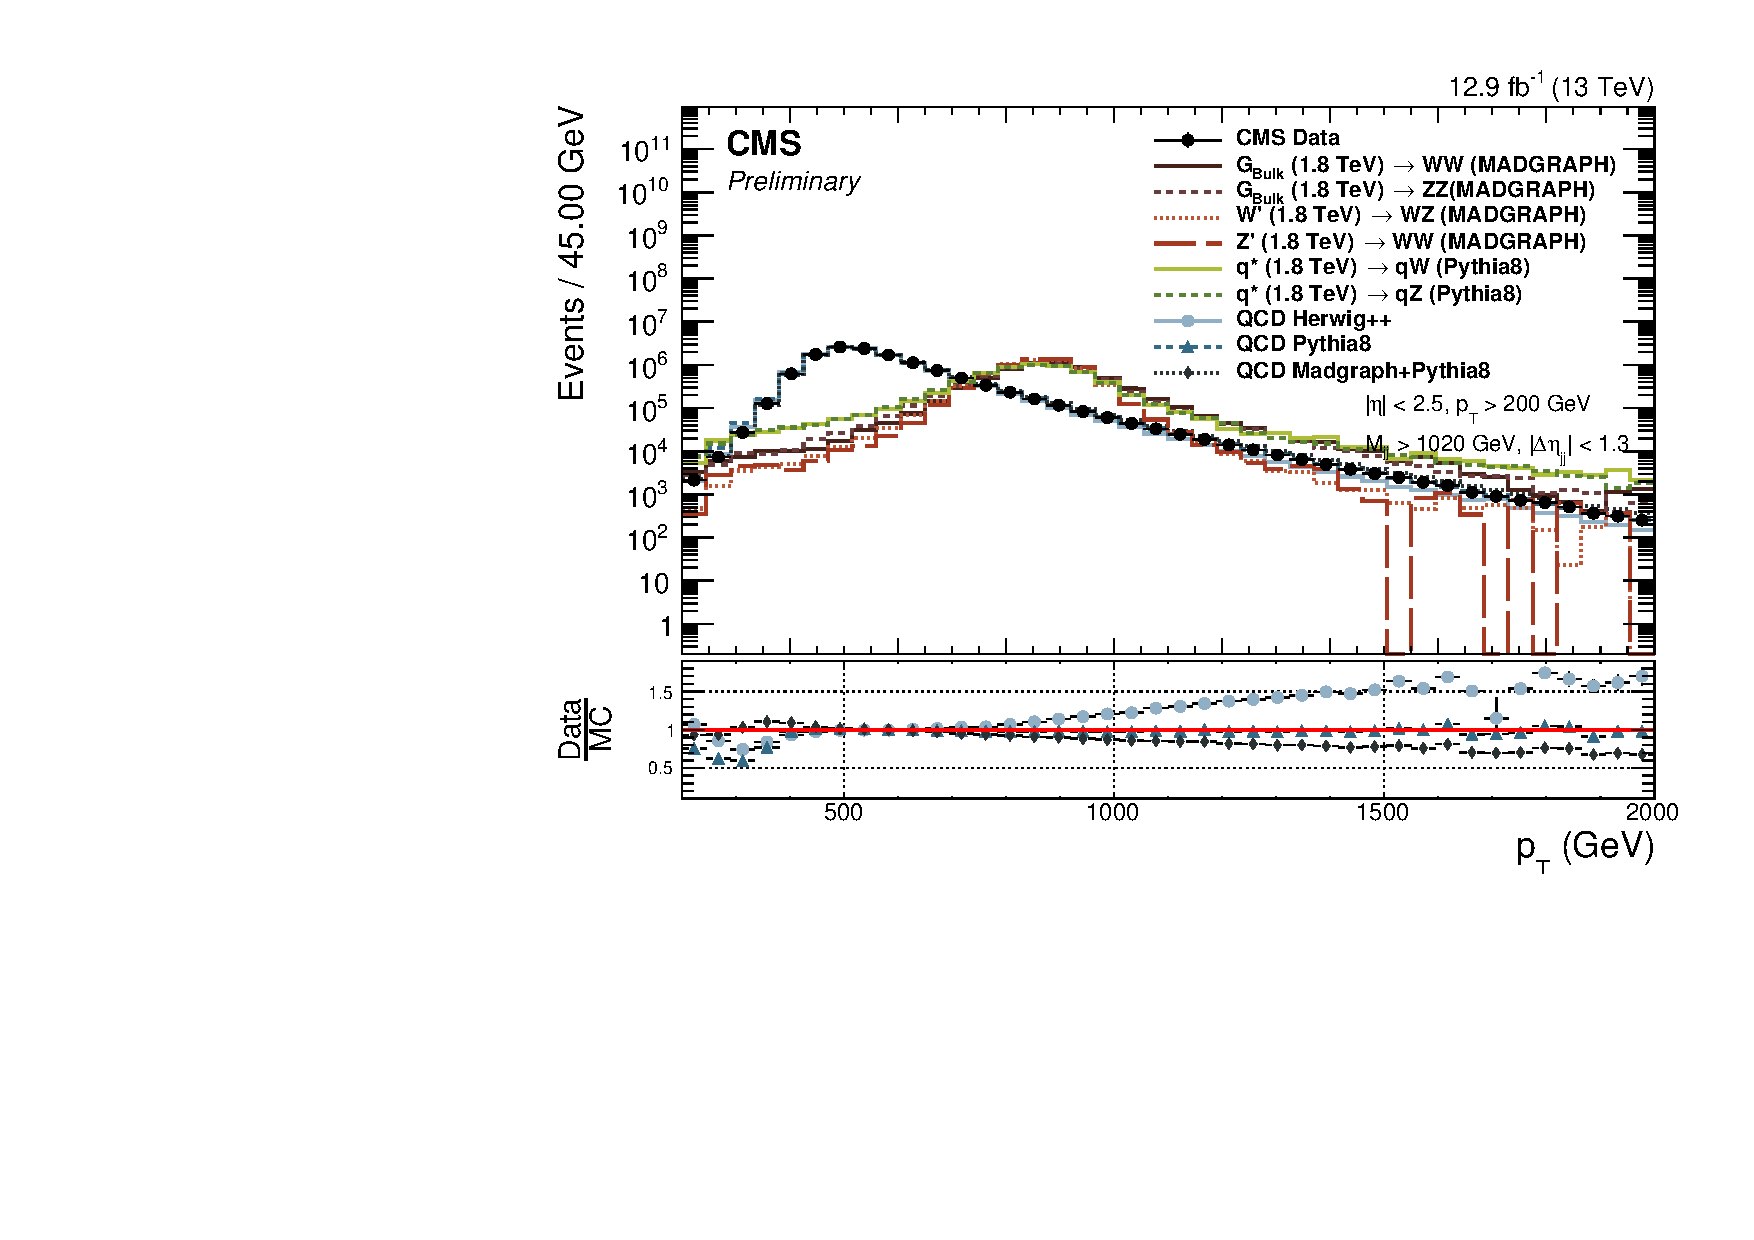
\includegraphics[width=0.49\textwidth]{figures/analysis/search2/AN-16-235/plots/qcdcp_Pt.pdf}
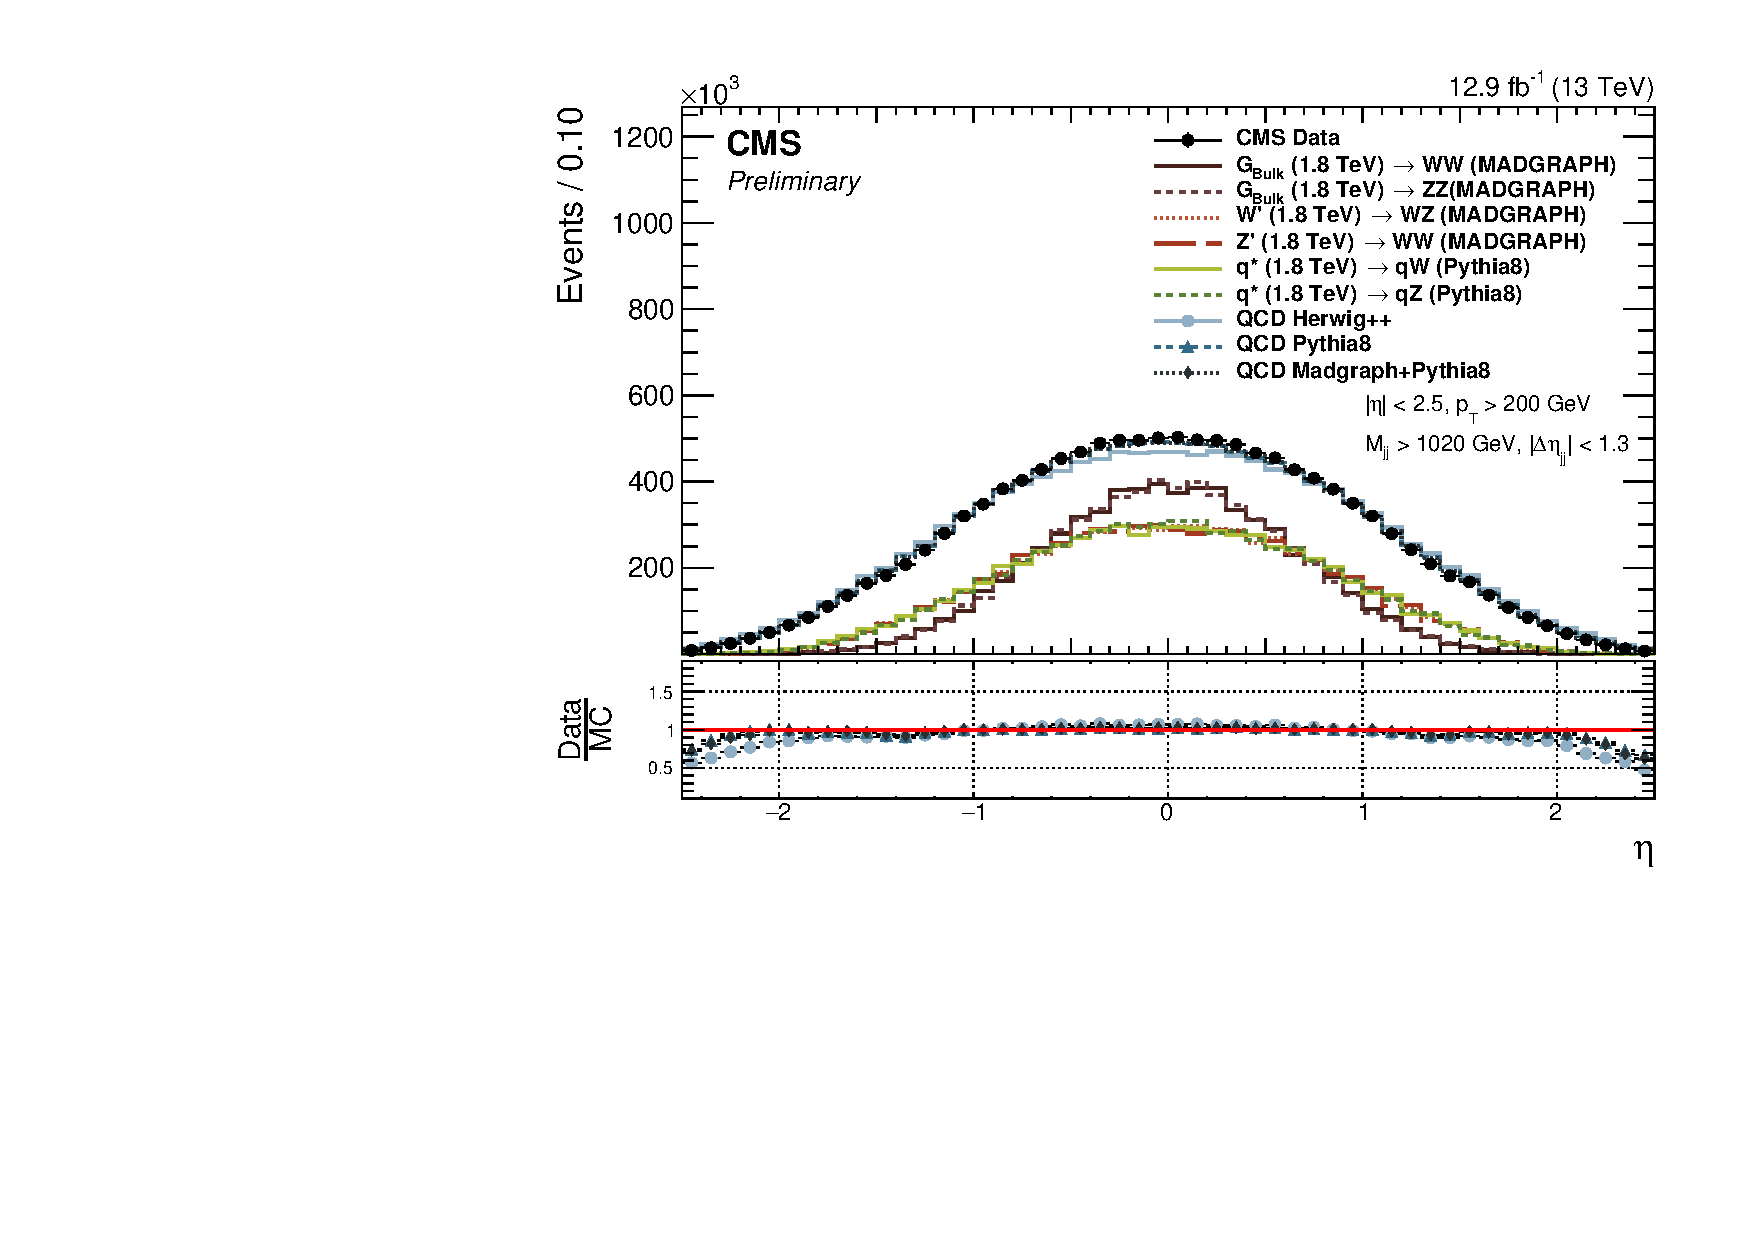
\includegraphics[width=0.49\textwidth]{figures/analysis/search2/AN-16-235/plots/qcdcp_Eta.pdf}\\
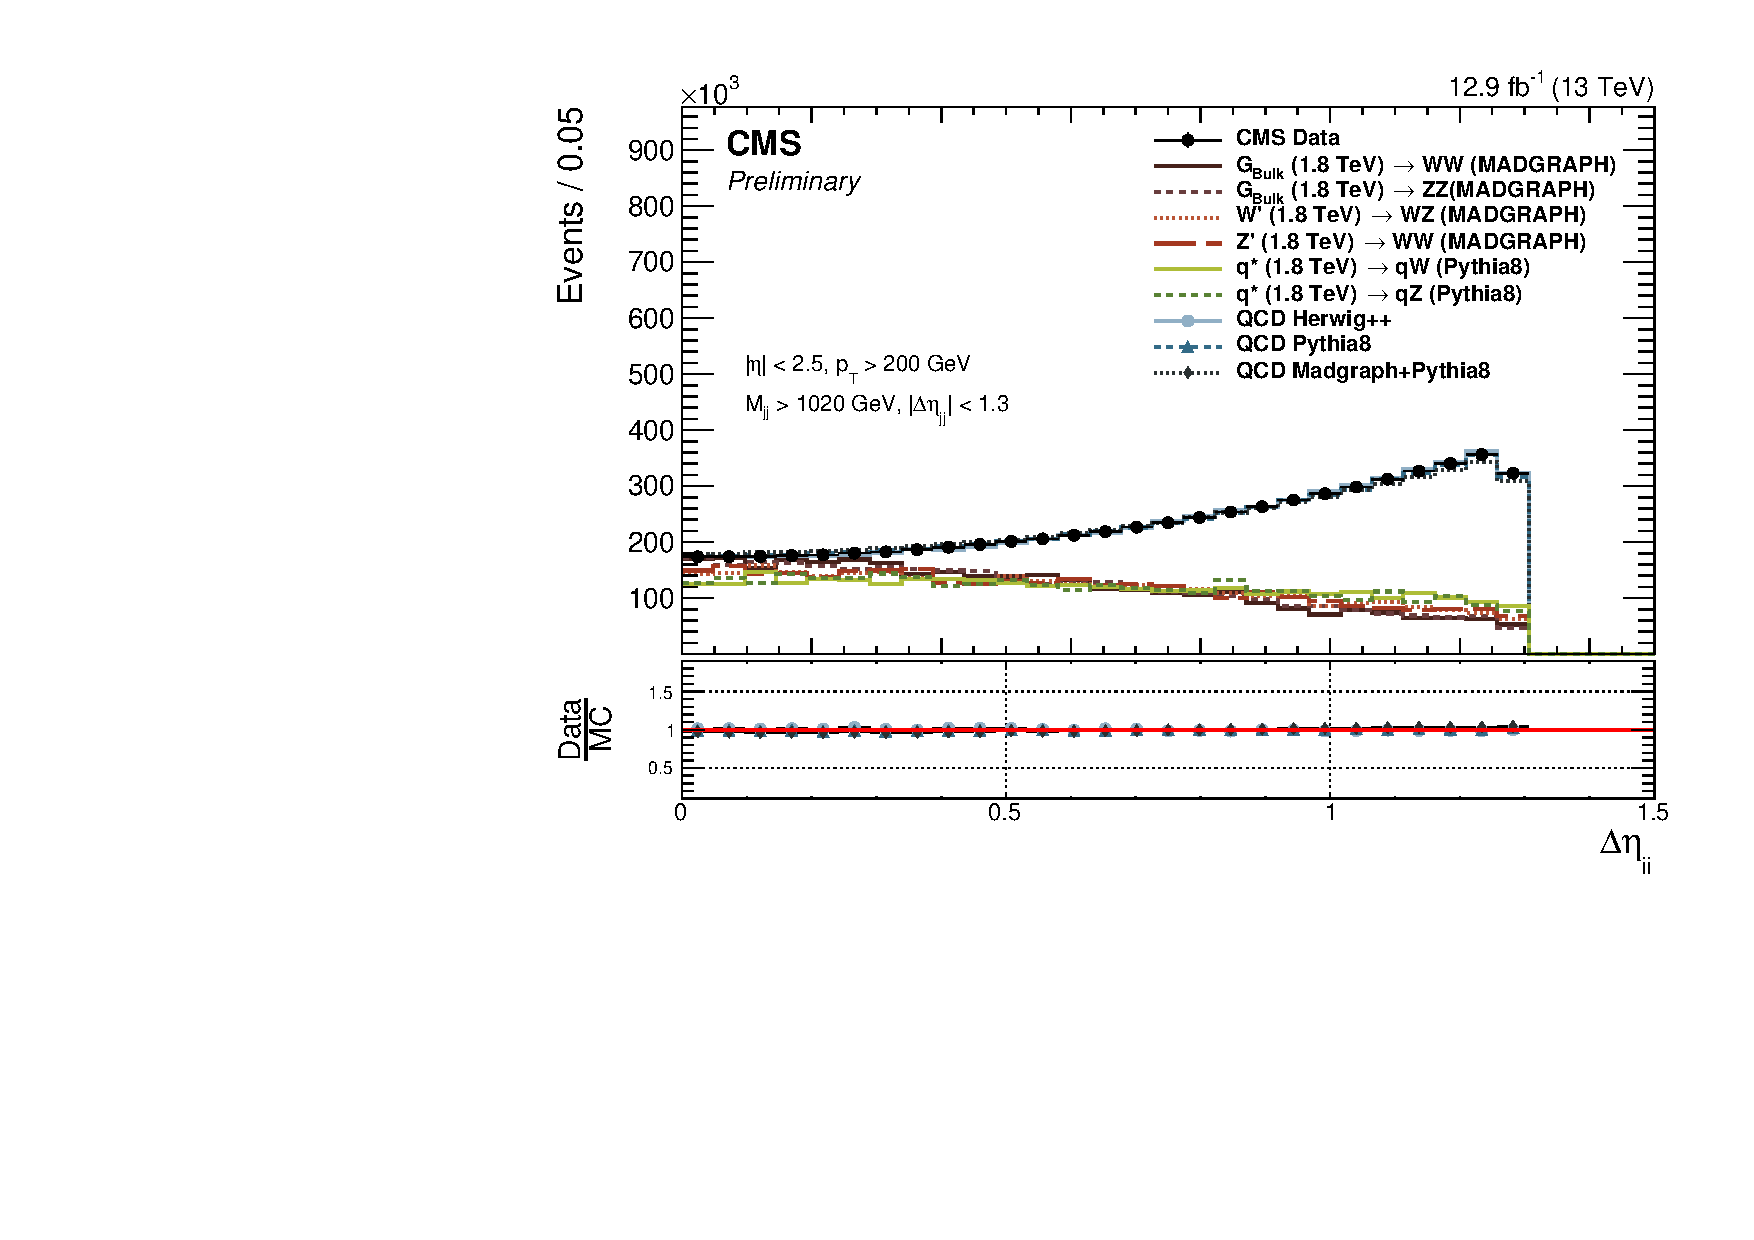
\includegraphics[width=0.49\textwidth]{figures/analysis/search2/AN-16-235/plots/qcdcp_DeltaEta.pdf}
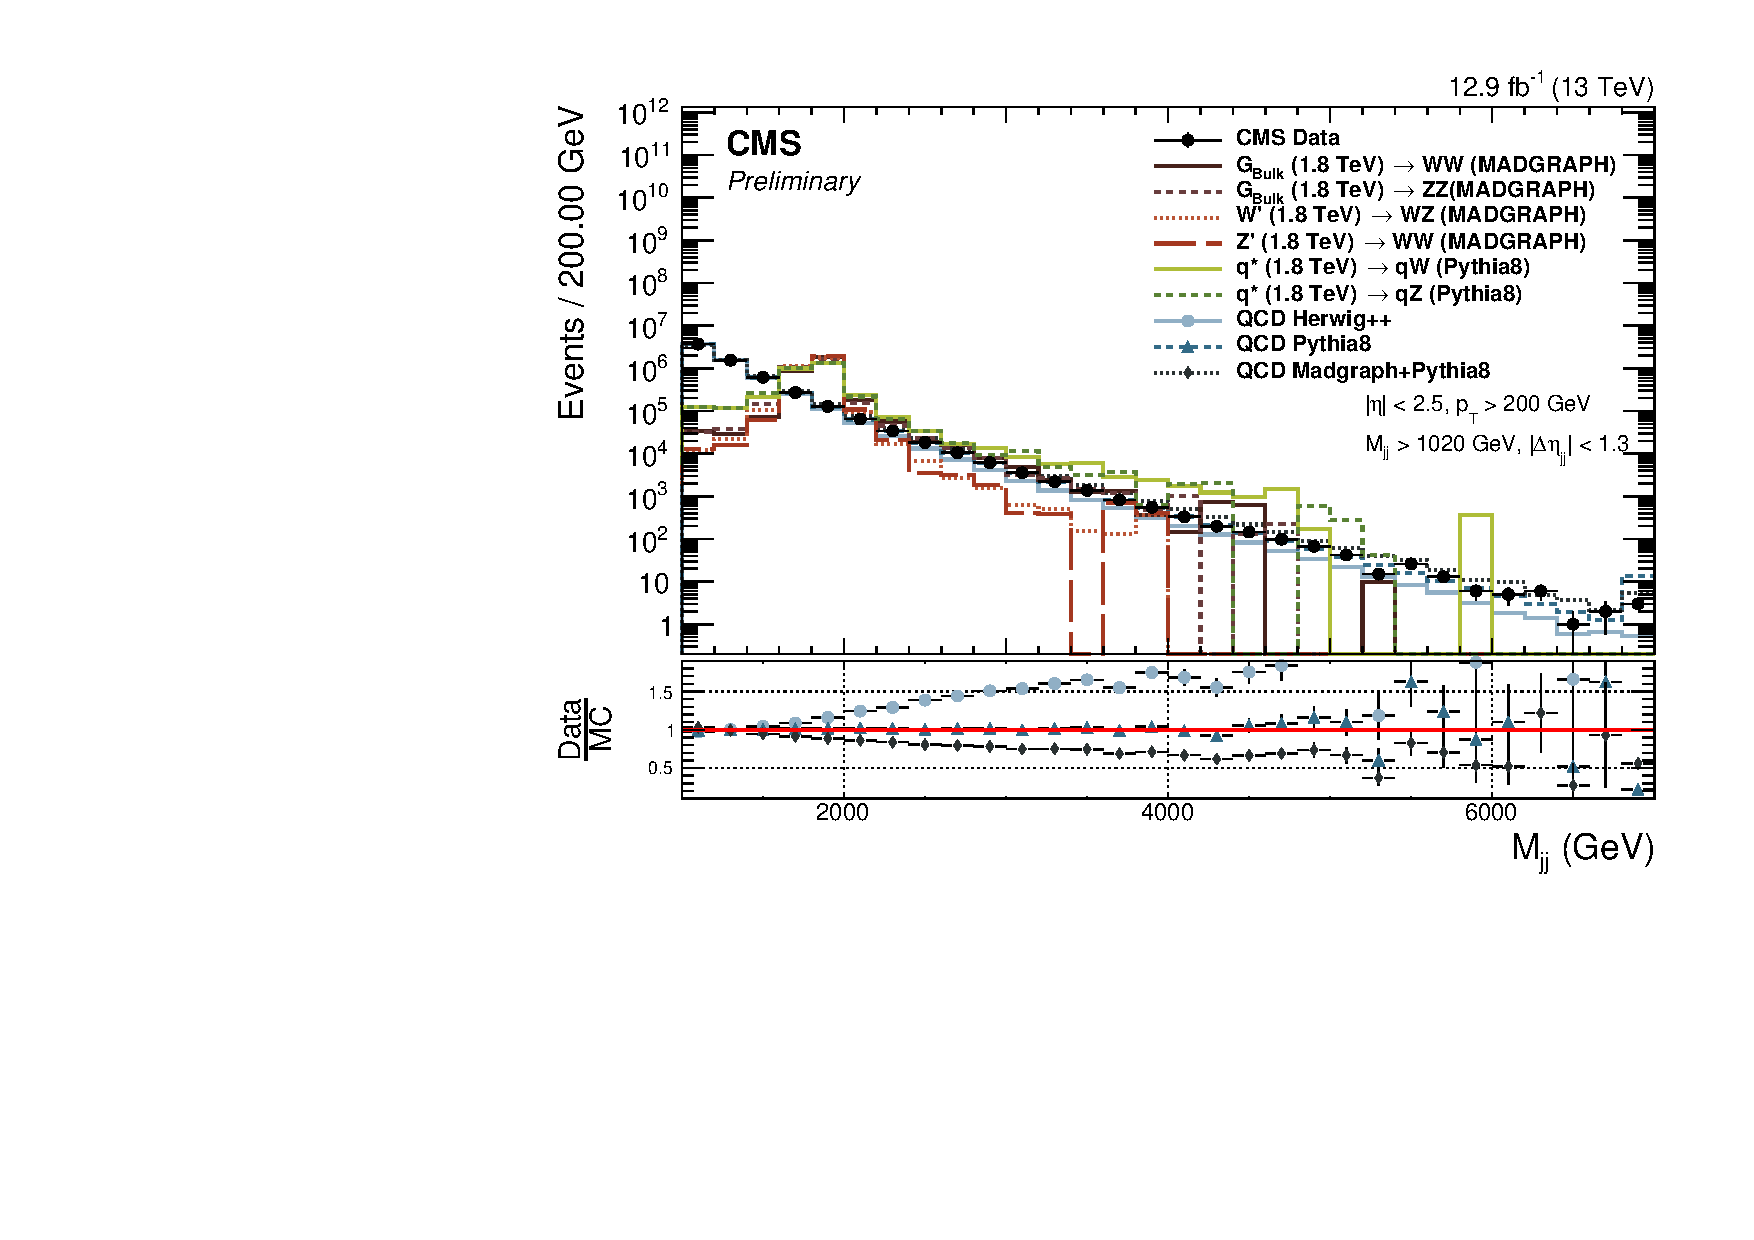
\includegraphics[width=0.49\textwidth]{figures/analysis/search2/AN-16-235/plots/qcdcp_Mjj.pdf}
\caption{Jet \PT{} (top left), $\eta$ (top right), $\Delta \eta_{jj}$ and dijet invariant mass (bottom left) for the two leading jets in the event after loose preselections are applied. The signal is scaled by an arbitrary number.}
\label{fig:searchII:kinematics-all}
\end{figure}
A large difference in slope in the jet \PT and dijet invariant mass spectrum depending on the QCD matrix element or shower generator is observed. Pure \PYTHIA QCD MC describes the data best, while \HERWIG{++} and \amcatnlo{}+\PYTHIA tend to under- or over-estimate the number of high $\PT/\mjj$ jets, respectively. Pure \PYTHIA QCD MC is therefore used for all background checks in this analysis.


\subsection{Developing a new W-tagger}
\label{sec:searchII:puppisoftdrop}
As mentioned in the introduction to this chapter, early studies had shown that the PUPPI pileup subtraction algorithm yielded superior resolution on large-cone jet observables like the jet mass. We therefore wanted to check whether the softdrop jet mass, and its observed sensitivity to the Underlying Event and pileup, would be improved if a better pileup subtraction algorithm was applied pre-clustering.\par
Two interesting observations were made. Softdrop used together with PUPPI pileup subtraction displayed a much smaller \PT-dependent shift than CHS+Softdrop, as hoped. Figure~\ref{fig:searchII:sdmass} shows the PUPPI softdrop mass for W-jets from a 1 \TeV ($\PT\sim 500 \GeV$) and 4 \TeV ($\PT\sim 2 \TeV$) resonance, exhibiting the desired reduced \PT dependence in jet mass scale. 
\begin{figure}[htb]
\centering
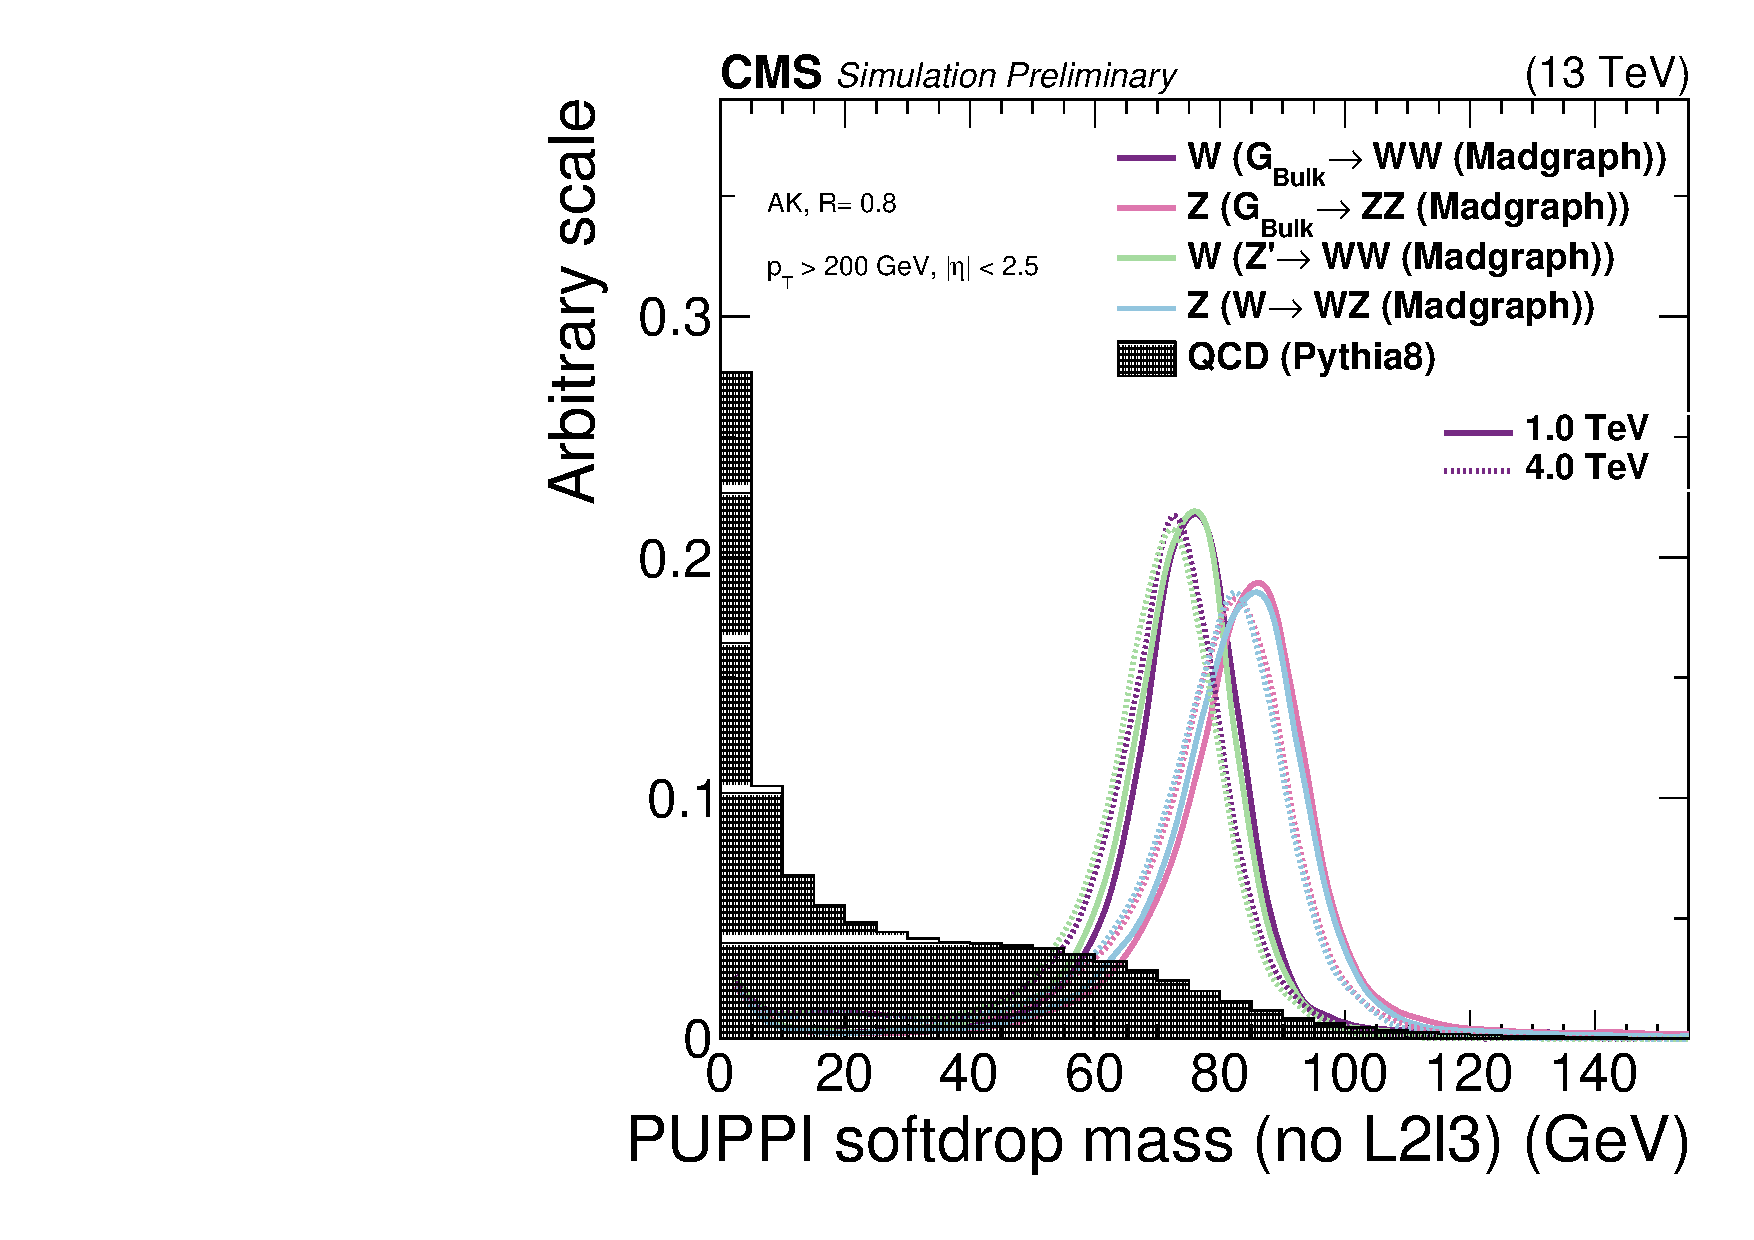
\includegraphics[width=0.49\textwidth]{figures/analysis/search2/AN-16-235/plots/gen_SoftdropMassUnCorr.pdf}
\caption{The  PUPPI softdrop jet mass distribution with no jet energy corrections applied}
\label{fig:searchII:sdmass}
\end{figure}
However, when applying centrally provided L2 and L3 jet energy corrections (see Section~\ref{sec:objreco:jec}) to the jet groomed mass, as is recommended, a strong \PT dependence is re-introduced. This effect is not present for the pruned jet mass. Figure~\ref{fig:searchII:wtagmass} show the softdrop (top left) and pruned (top right) jet mass distribution with recommended L2L3 corrections applied. Here, the PUPPI+softdrop jet mass shift is significantly increased with respect to what was observed for the uncorrected mass, while CHS+pruned jet mass is stable. This points to the PUPPI jet energy corrections not being optimal for scalar jet mass variables, while they may be good for correcting jet 4-vectors. The jet energy corrections derived for CHS and PUPPI jets as a function of jet \PT is shown in the bottom plot in Figure~\ref{fig:searchII:wtagmass} . A significant slope in JEC as a function of \PT is measured for PUPPI, while not present for CHS.
\begin{figure}[htb]
\centering
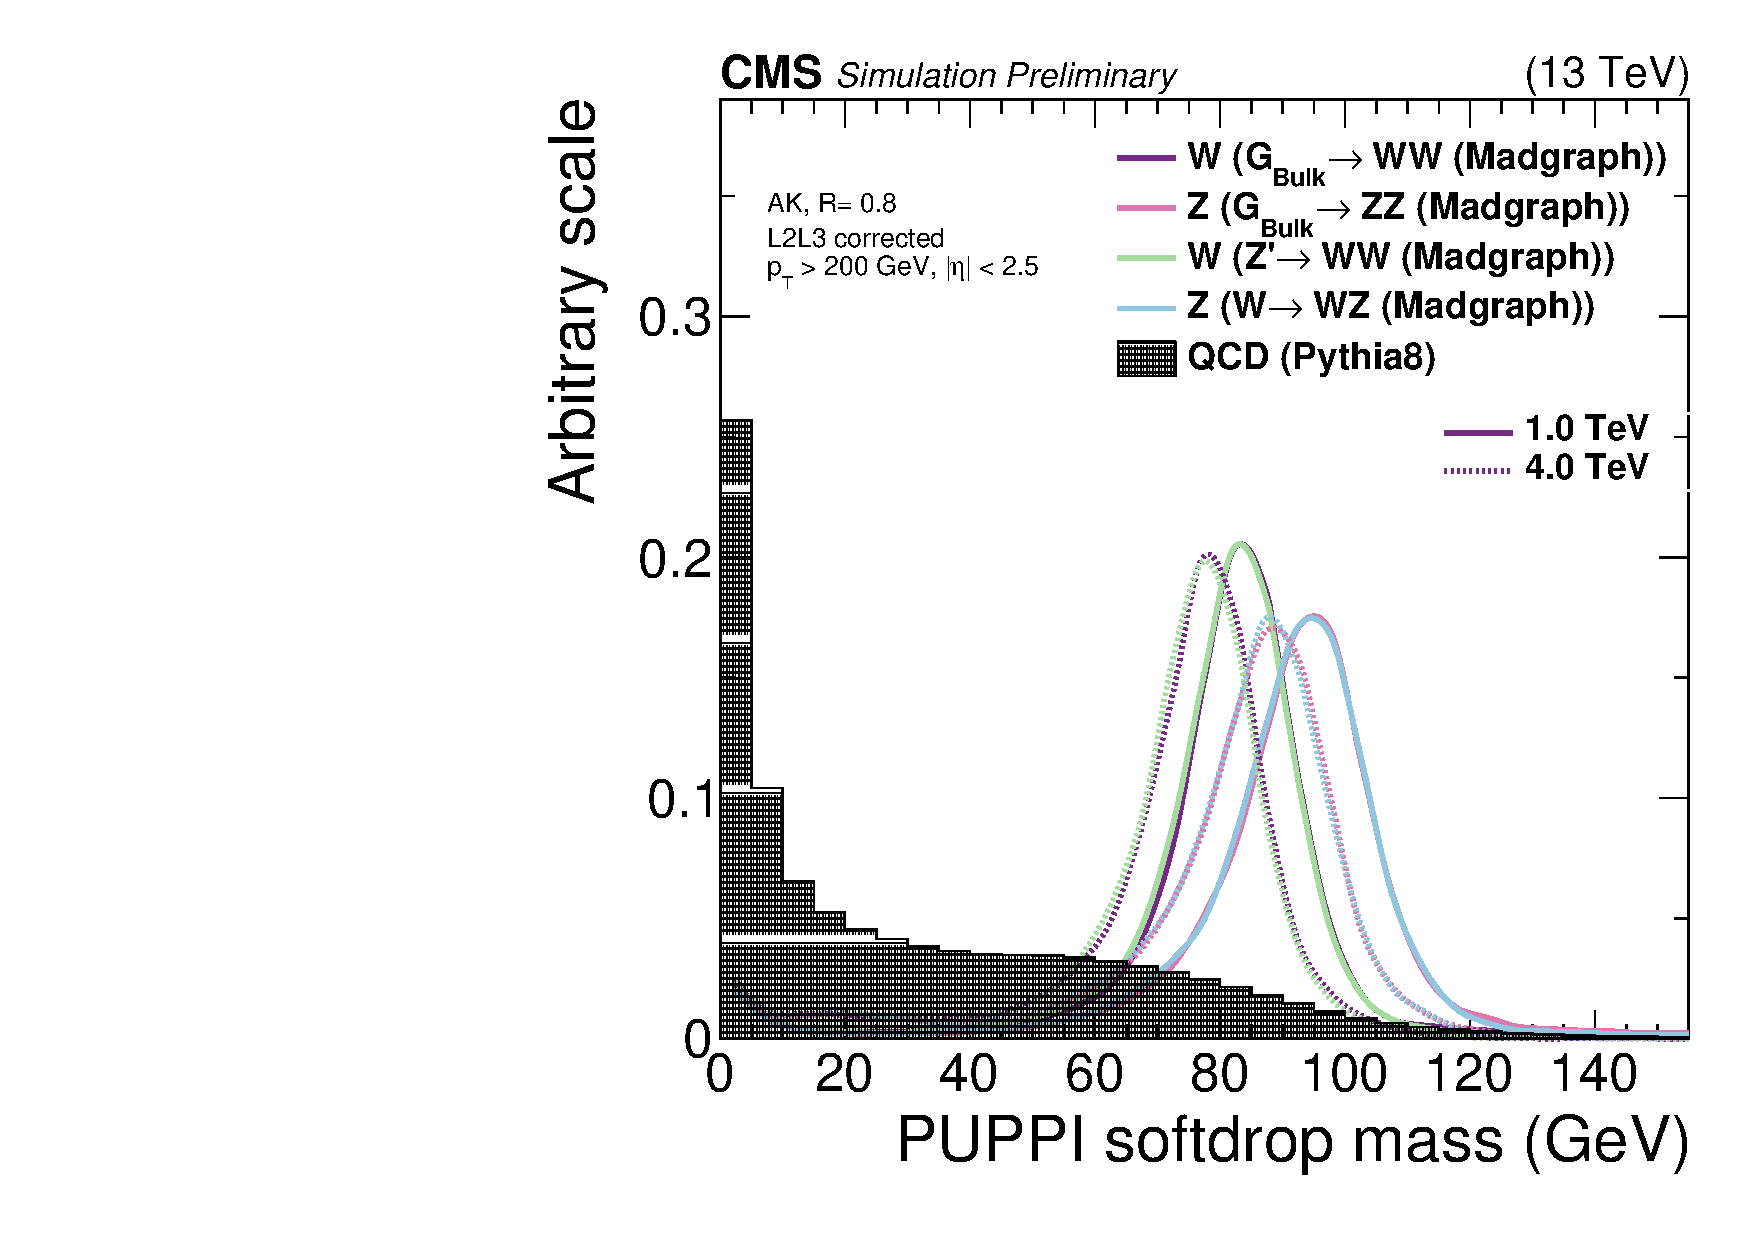
\includegraphics[width=0.49\textwidth]{figures/analysis/search2/AN-16-235/plots/gen_SoftdropMass.pdf}
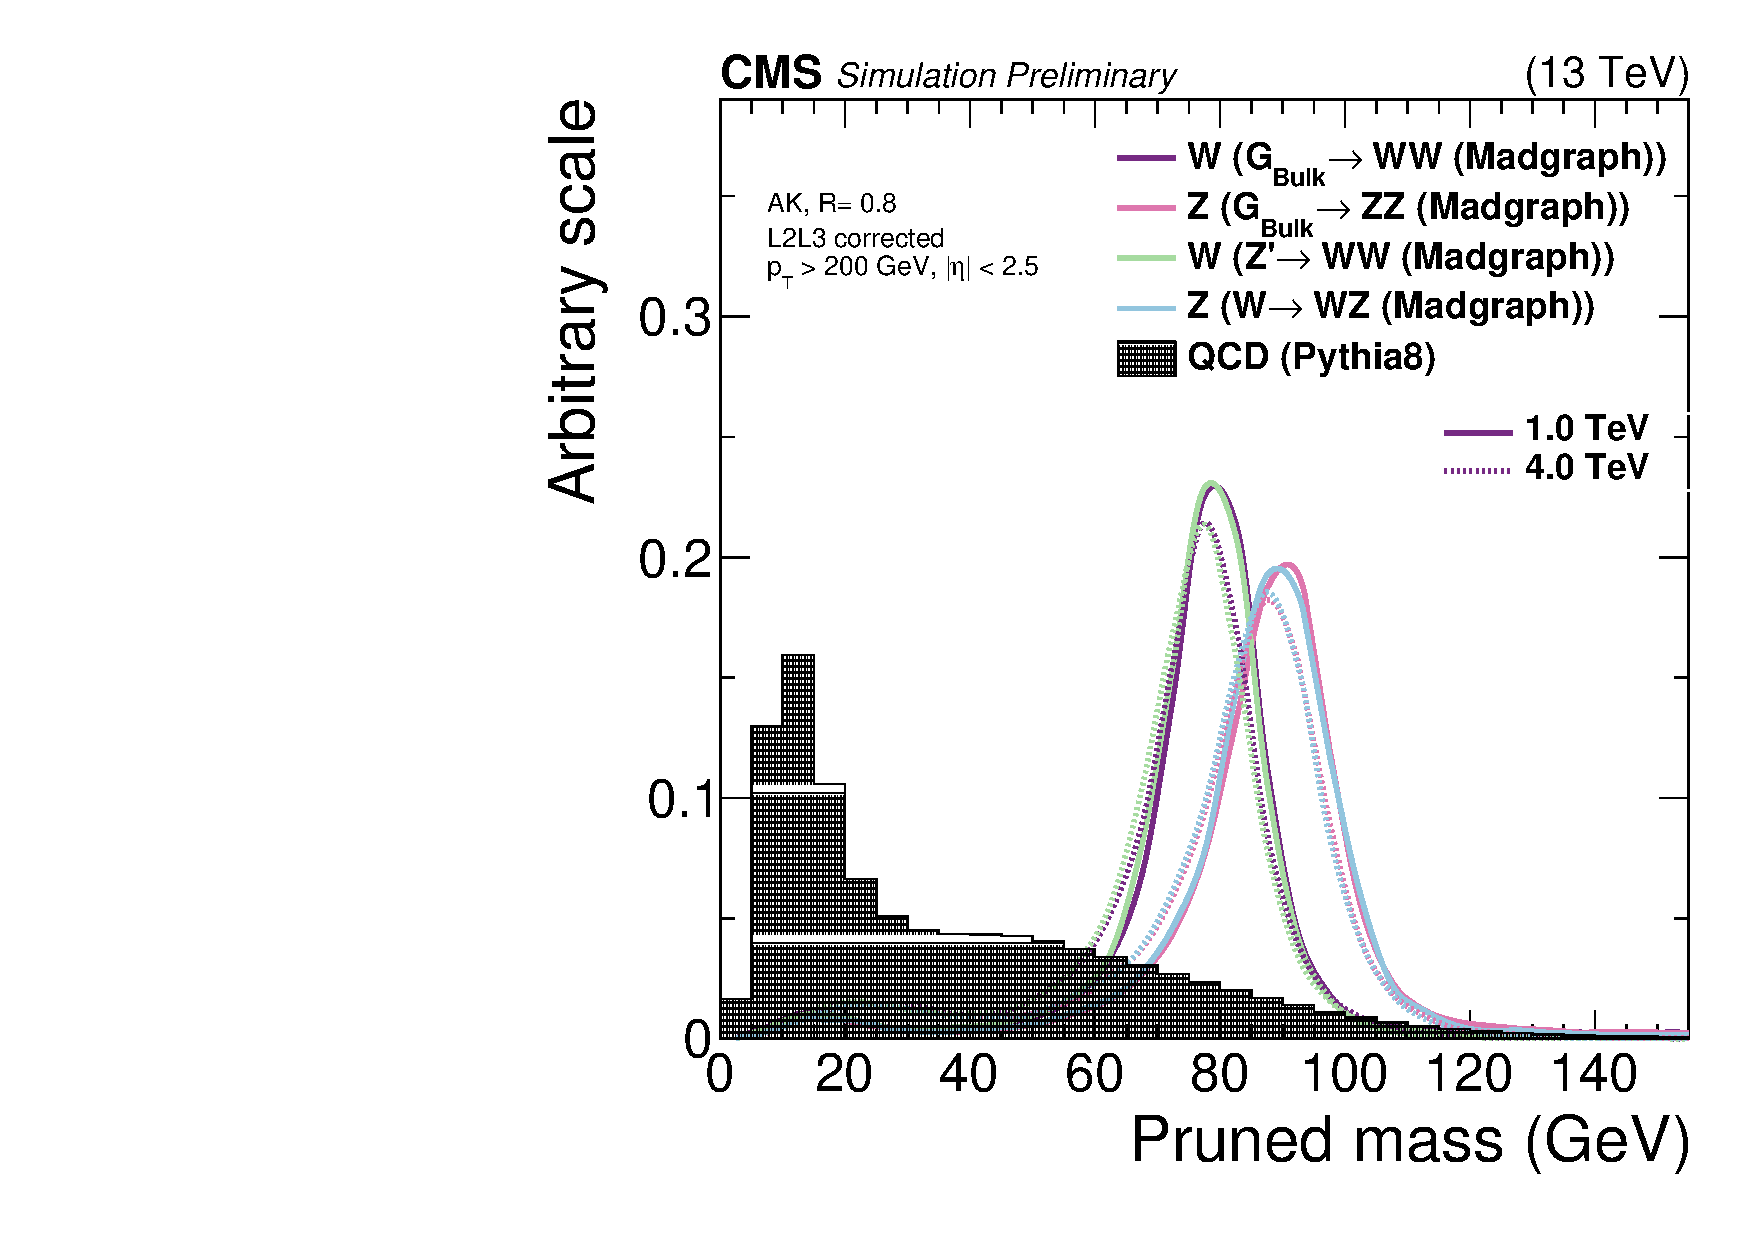
\includegraphics[width=0.49\textwidth]{figures/analysis/search2/AN-16-235/plots/gen_PrunedMass.pdf}\\
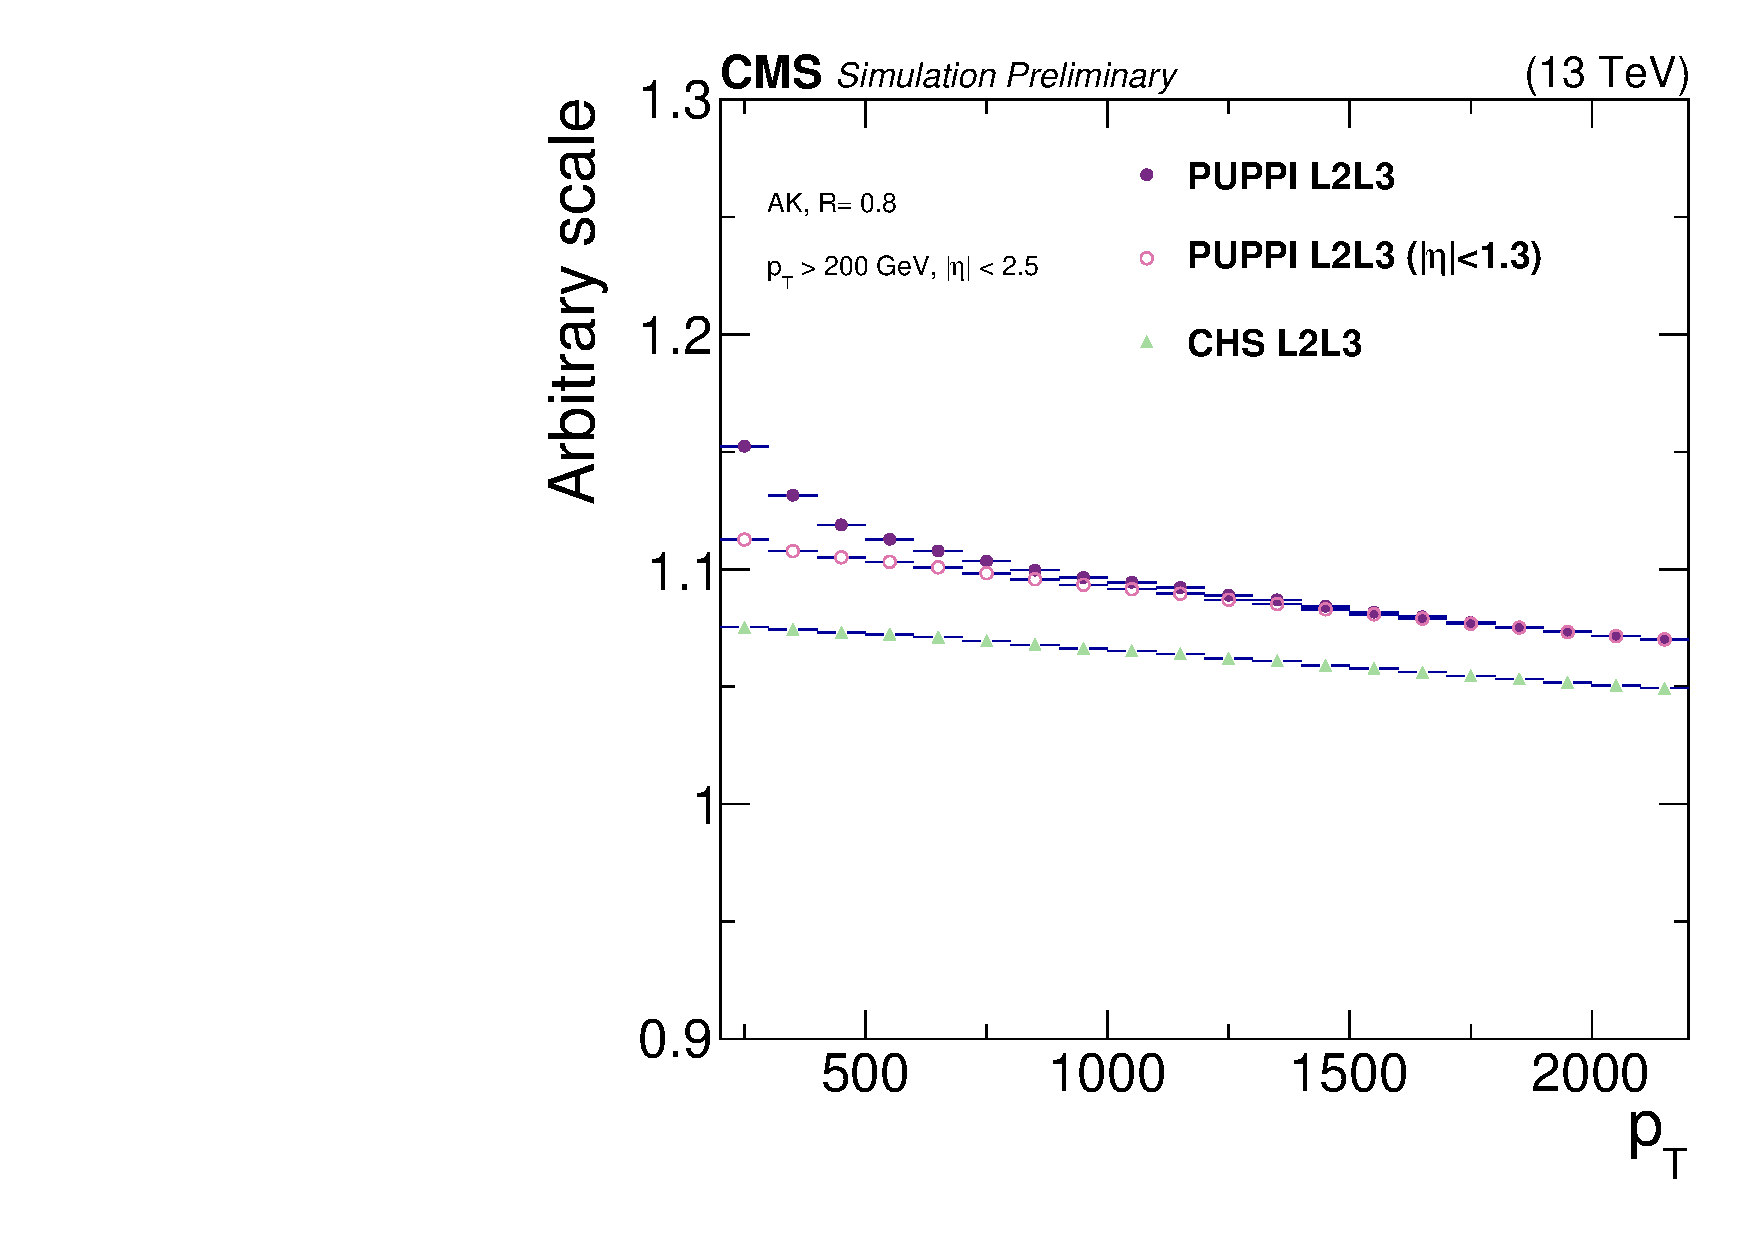
\includegraphics[width=0.49\textwidth]{figures/analysis/search2/AN-16-235/plots/JECvsPT.pdf}
\caption{Top: PUPPI softdrop mass distribution (top left) and pruned jet mass distribution (top right) with L2 and L3 corrections applied. Bottom: The projection of CHS and PUPPI jet energy corrections versus jet \PT.}
\label{fig:searchII:wtagmass}
\end{figure}

\subsubsection{Dedicated PUPPI softdrop mass corrections}
\label{sec:searchII:masscorr}
In order to minimize \PT dependence in the PUPPI softdrop jet mass, all jet energy corrections to the softdrop jet mass are removed. However, this still leaves a residual \PT dependence and, in addition, the uncorrected mass does not peak at the correct W-mass of 80.4~\GeV. Figure~\ref{fig:searchII:UncorrSD} shows the mean of a Gaussian fit to the uncorrected PUPPI softdrop mass as a function of jet $\pt$ in two different $\eta$ bins (smaller or greater than $|\eta|=1.3$) for W-jets coming from a Bulk Graviton signal sample. A mass shift both as a function of $\eta$ and \PT is observed, together with an average mean significantly lower than the W-mass.
\begin{figure}[htbp]
\centering
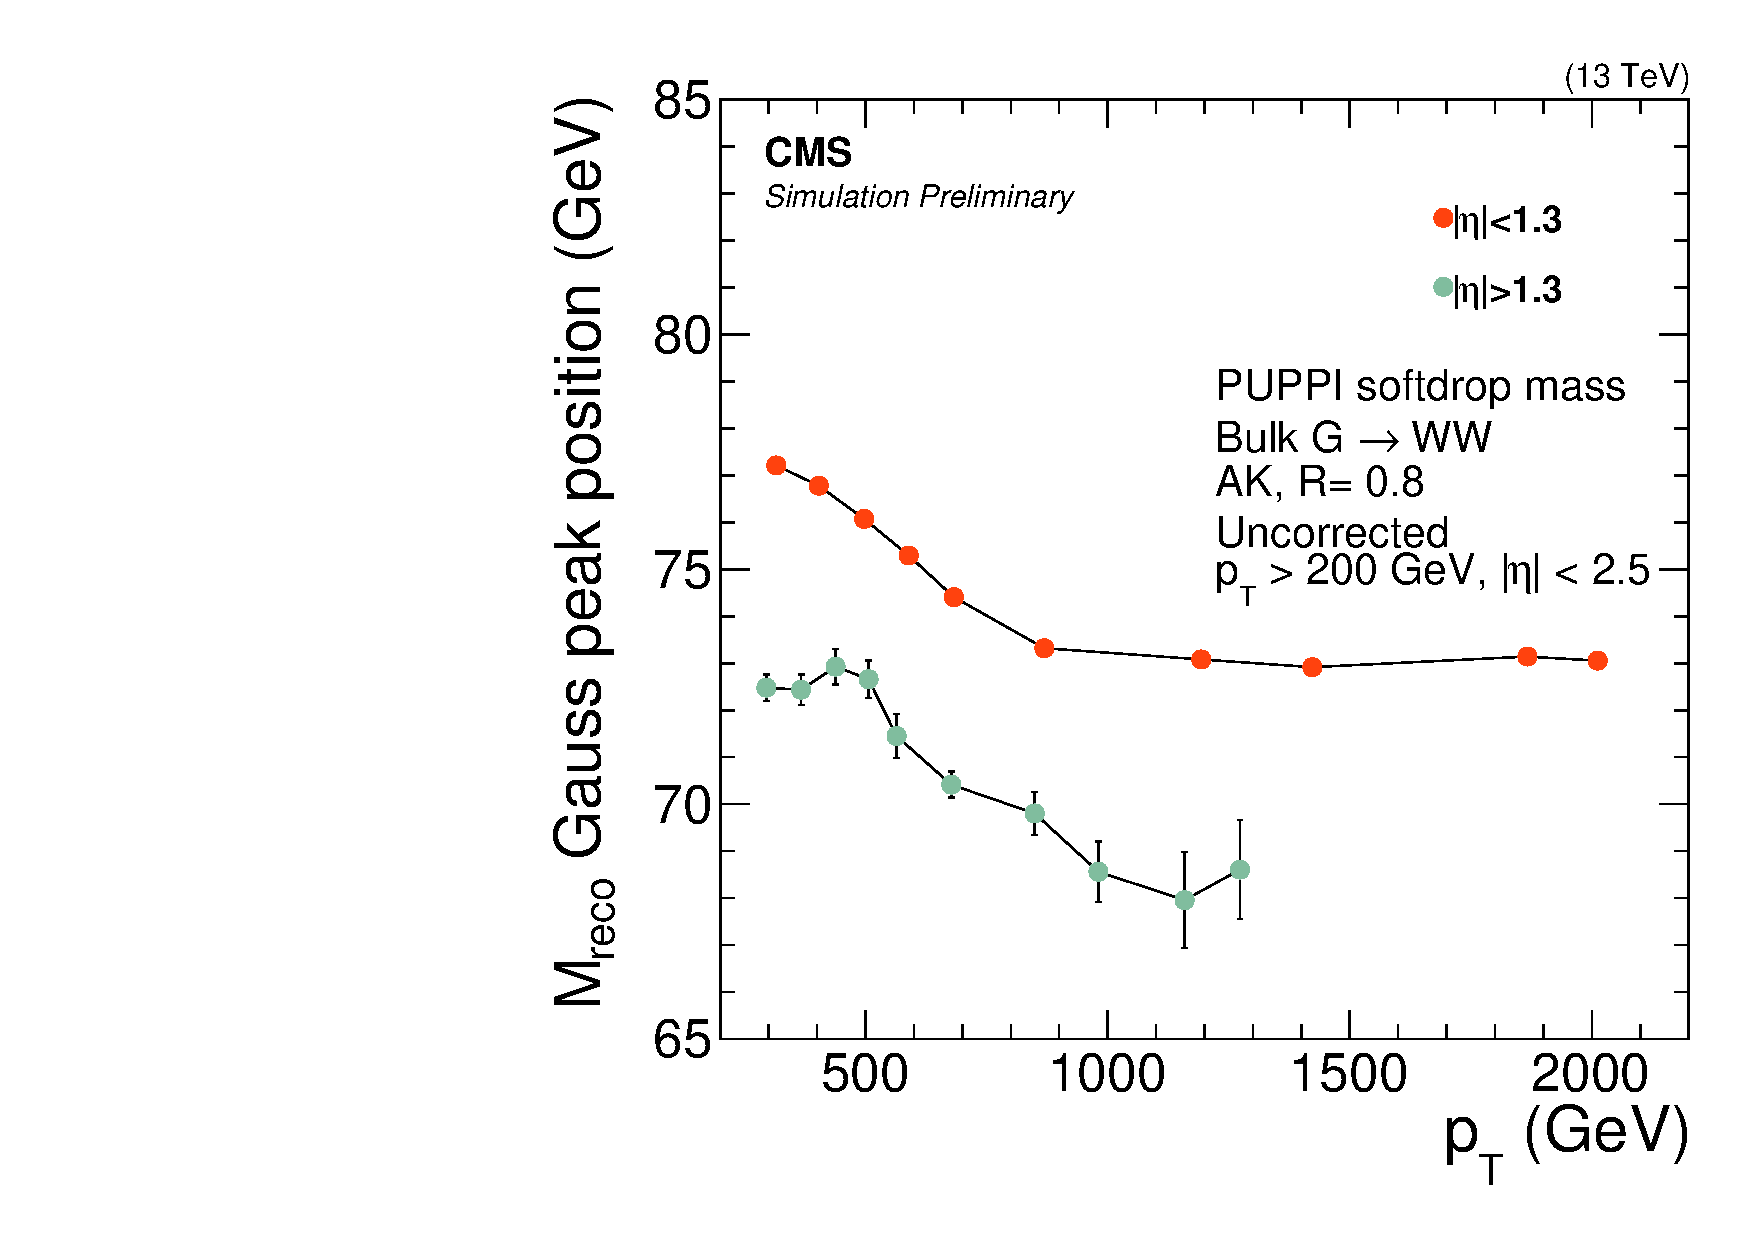
\includegraphics[width=0.49\textwidth]{figures/analysis/search2/AN-16-235/plots/RecoPuppiSoftdropMass_vspt.pdf}
\caption{The mean of a Gaussian fit to the W-jet PUPPI softdrop mass peak as a function of jet \PT in two different $\eta$ bins (smaller or greater than $|\eta|=1.3$). No corrections have been applied to the softdrop mass.}
\label{fig:searchII:UncorrSD}
\end{figure}
In order to use PUPPI+softdrop for W-tagging, we therefore derive dedicated jet mass corrections to compensate for two factors: A generator level \PT-dependence, as first observed in \label{sec:searchI:wtagging}, and a reconstruction level \PT- and $\eta$-dependence, most likely caused by UE effects and the growing effective sofdrop radius at low jet \PT. Figure~\ref{fig:searchII:sdmassshifts} shows the mean of the generated softdrop mass (left) and the normalized difference in reconstructed and generated softdrop mass (right) as a function of jet \PT. The shift in generated softdrop mass at lower \PT is of the order of 2-3$\%$ while the difference between reconstructed and generated softdrop mass is a 5-10$\%$ effect.
\begin{figure}[htbp]
\centering
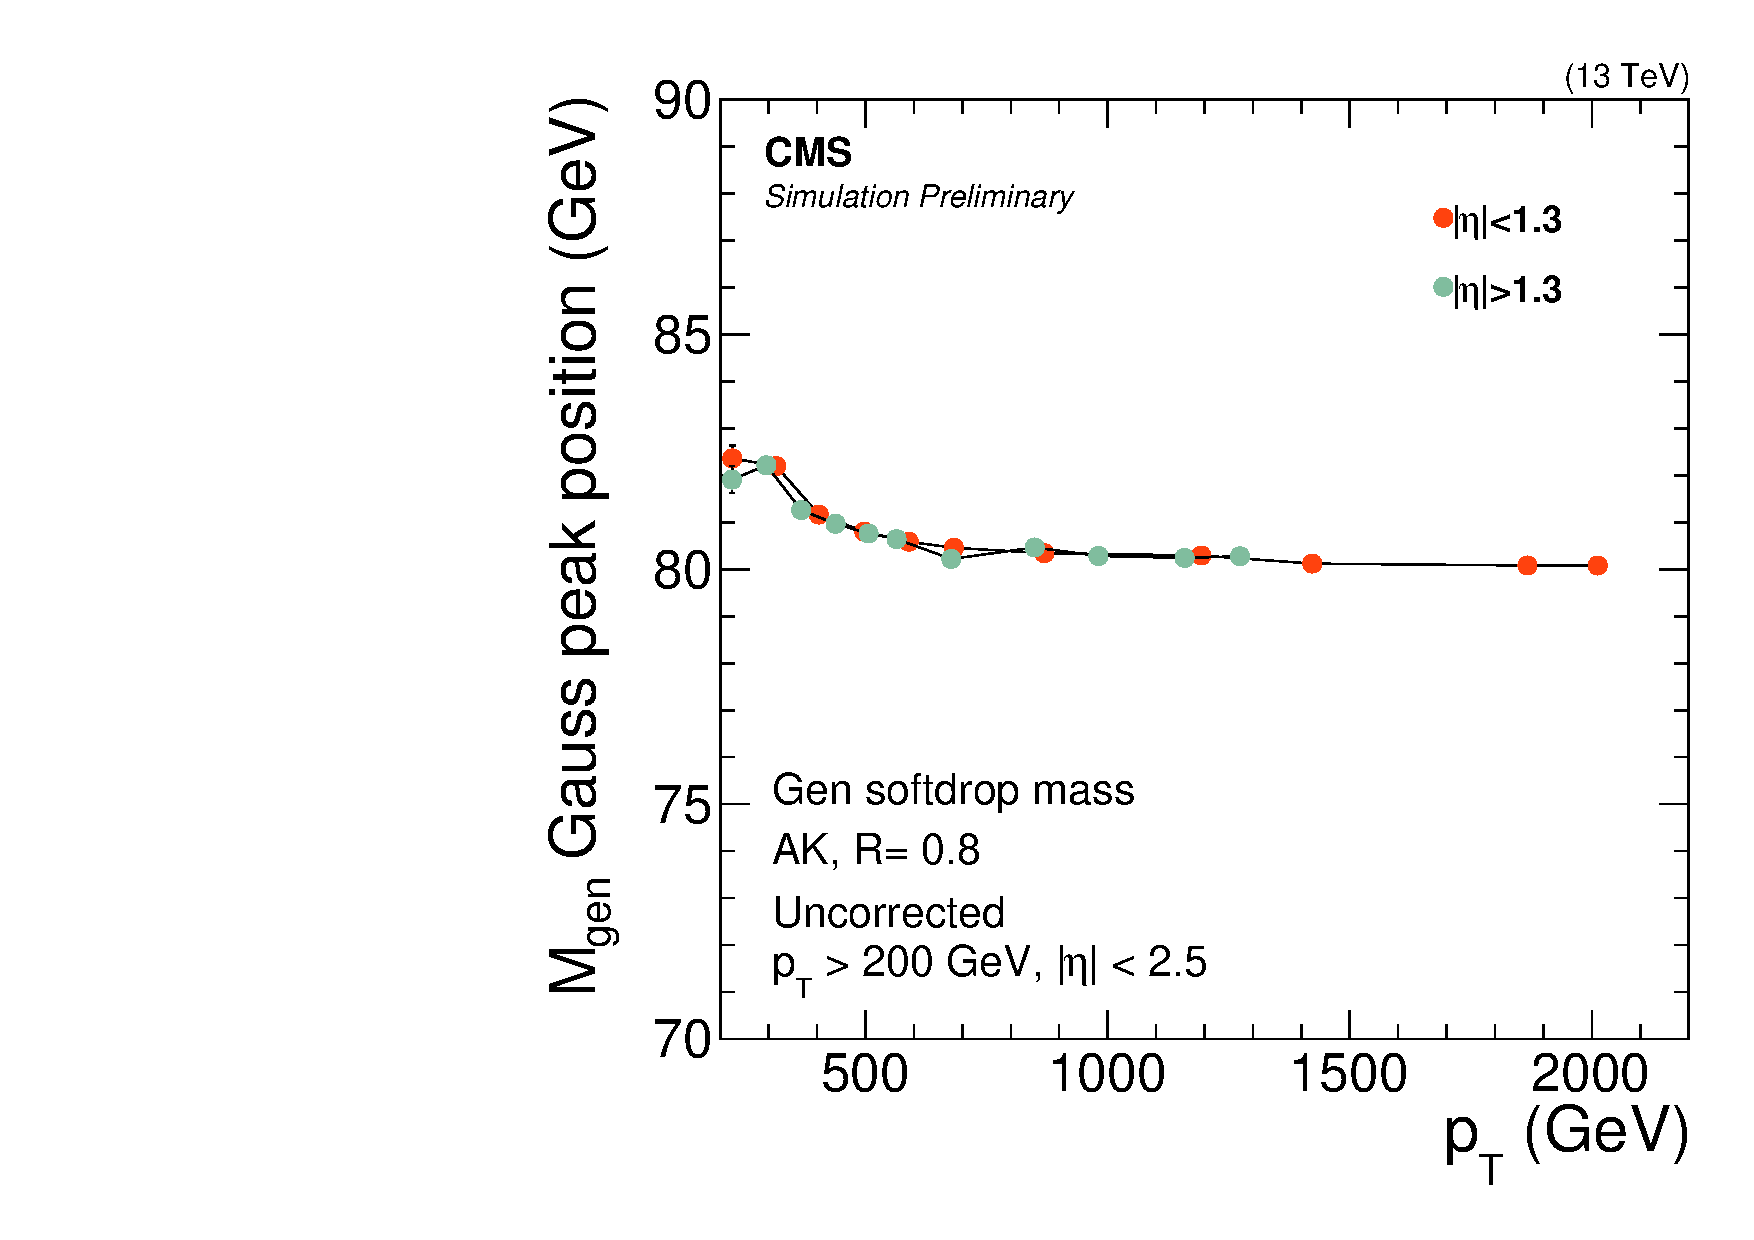
\includegraphics[width=0.49\textwidth]{figures/analysis/search2/AN-16-235/plots/GenSoftdropMass_vspt.pdf}
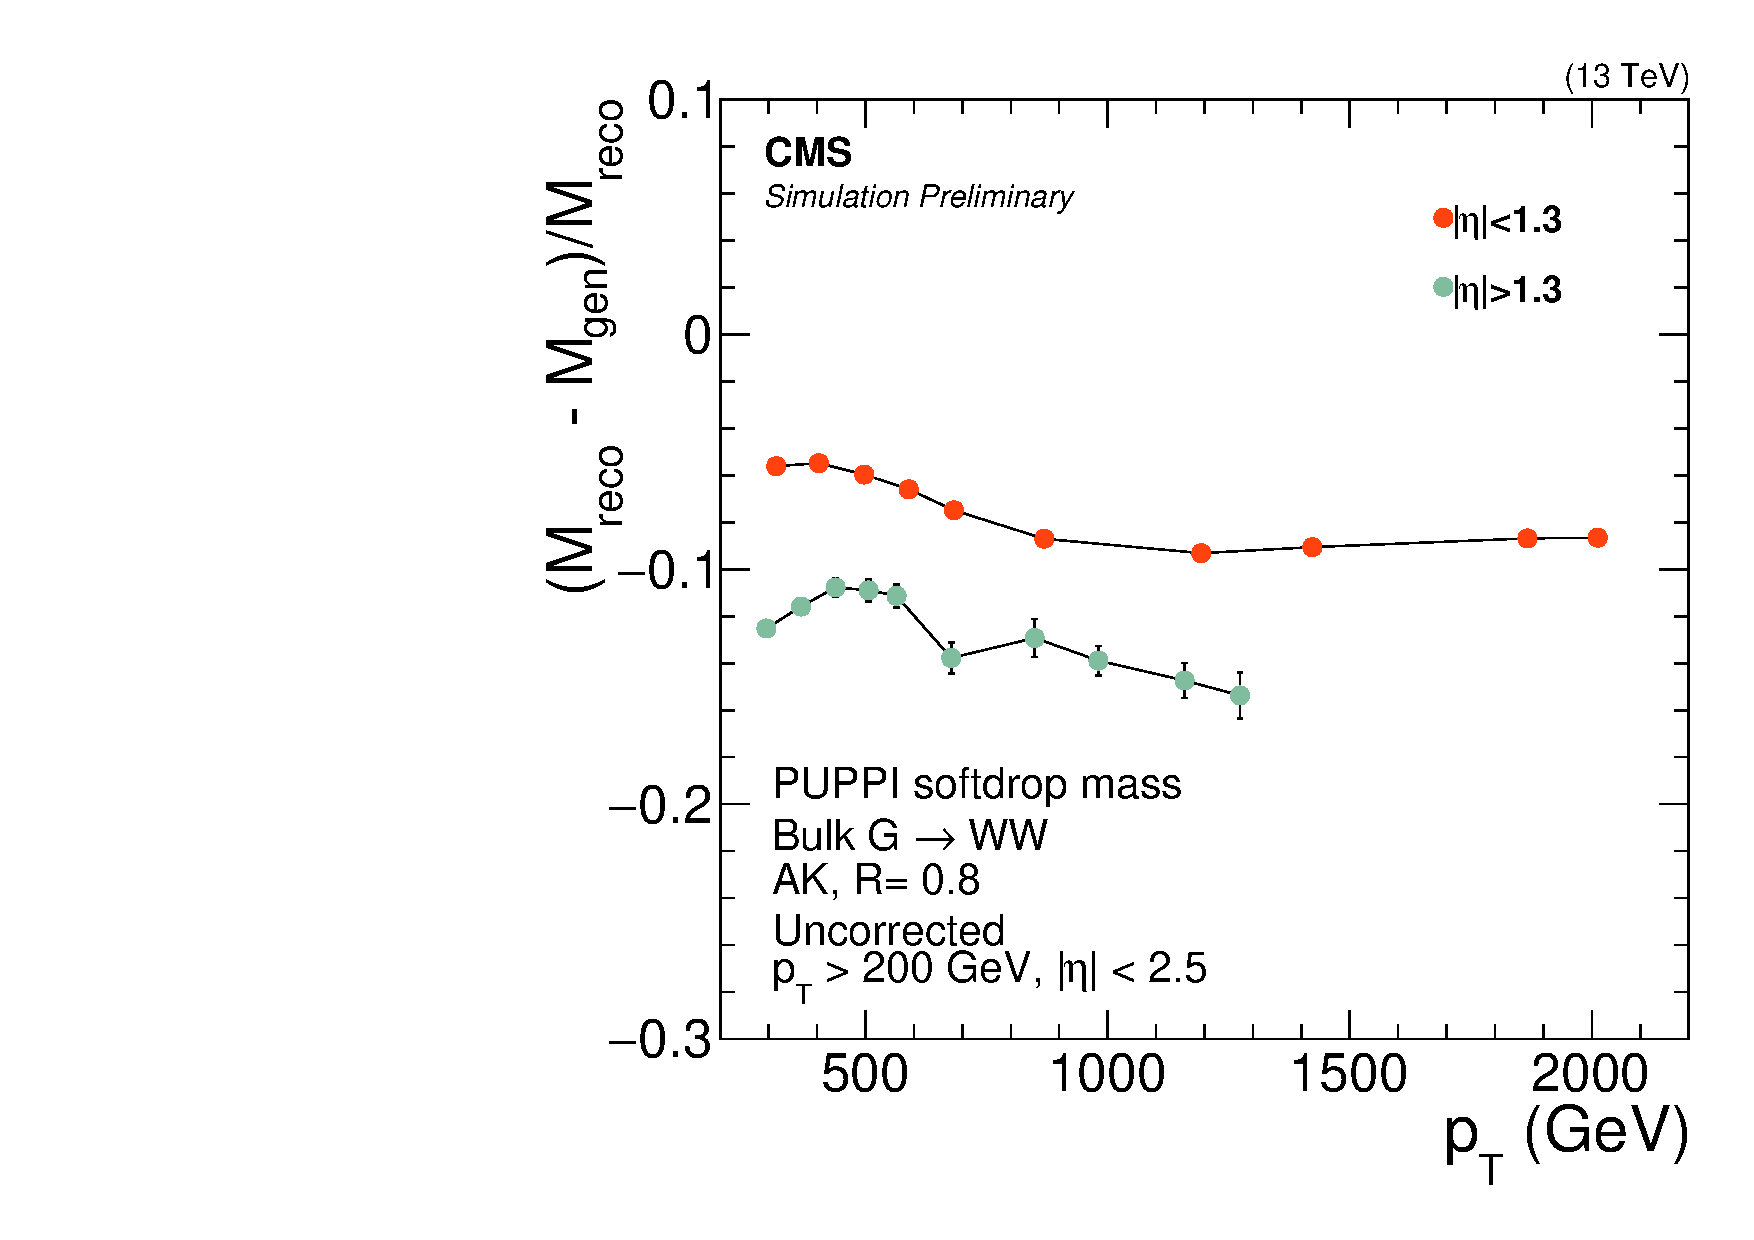
\includegraphics[width=0.49\textwidth]{figures/analysis/search2/AN-16-235/plots/MassShift_vspt.pdf}
\caption{The mean of the fitted generator level W-jet softdrop mass distribution as a function of jet $\pt$ (left) and the normalized difference in reconstructed and generated softdrop mass (right).}
\label{fig:searchII:sdmassshifts}
\end{figure}
The mass shift introduced at generator level is corrected by a fit to $\rm{M_{PDG}/M_{GEN}}$ as a function of jet \PT, where $\rm{M_{PDG}}=80.4~\GeV$ and $\rm{M_{GEN}}$ is the fitted mean of the generator level mass as shown in the left plot in Figure~\ref{fig:searchII:sdmassshifts}. To correct for the residual shift between generated and reconstructed softdrop mass, a fit to $\rm{(M_{RECO}-M_{GEN})/M_{RECO}}$, where $\rm{M_{RECO}}$ is the reconstructed mass shown in the right plot in Figure~\ref{fig:searchII:sdmassshifts} and $\rm{M_{GEN}}$ is as defined above, as a function of jet \PT in two $\eta$ bins (smaller or greater than $|\eta|=1.3$) is performed.
Polynomial fit functions of the following forms are used
\begin{align*} 
% w(\pt) &=  [0]+[1]*pow(x*[2],-[3] \\
w(\pt) &=  A  +B(x^{2})^{-C}          &\sim\textrm{``gen correction''}\\
w(\pt) &=  A  +Bx+Cx^2+Dx^3+Ex^4+Fx^5 &\sim\textrm{``reco correction''} 
\end{align*}
The distribution and corresponding fits for the two weights is shown in Figure~\ref{fig:jmcfits} for the "gen correction" (left) and "reco correction" (right).
\begin{figure}[htbp]
\centering
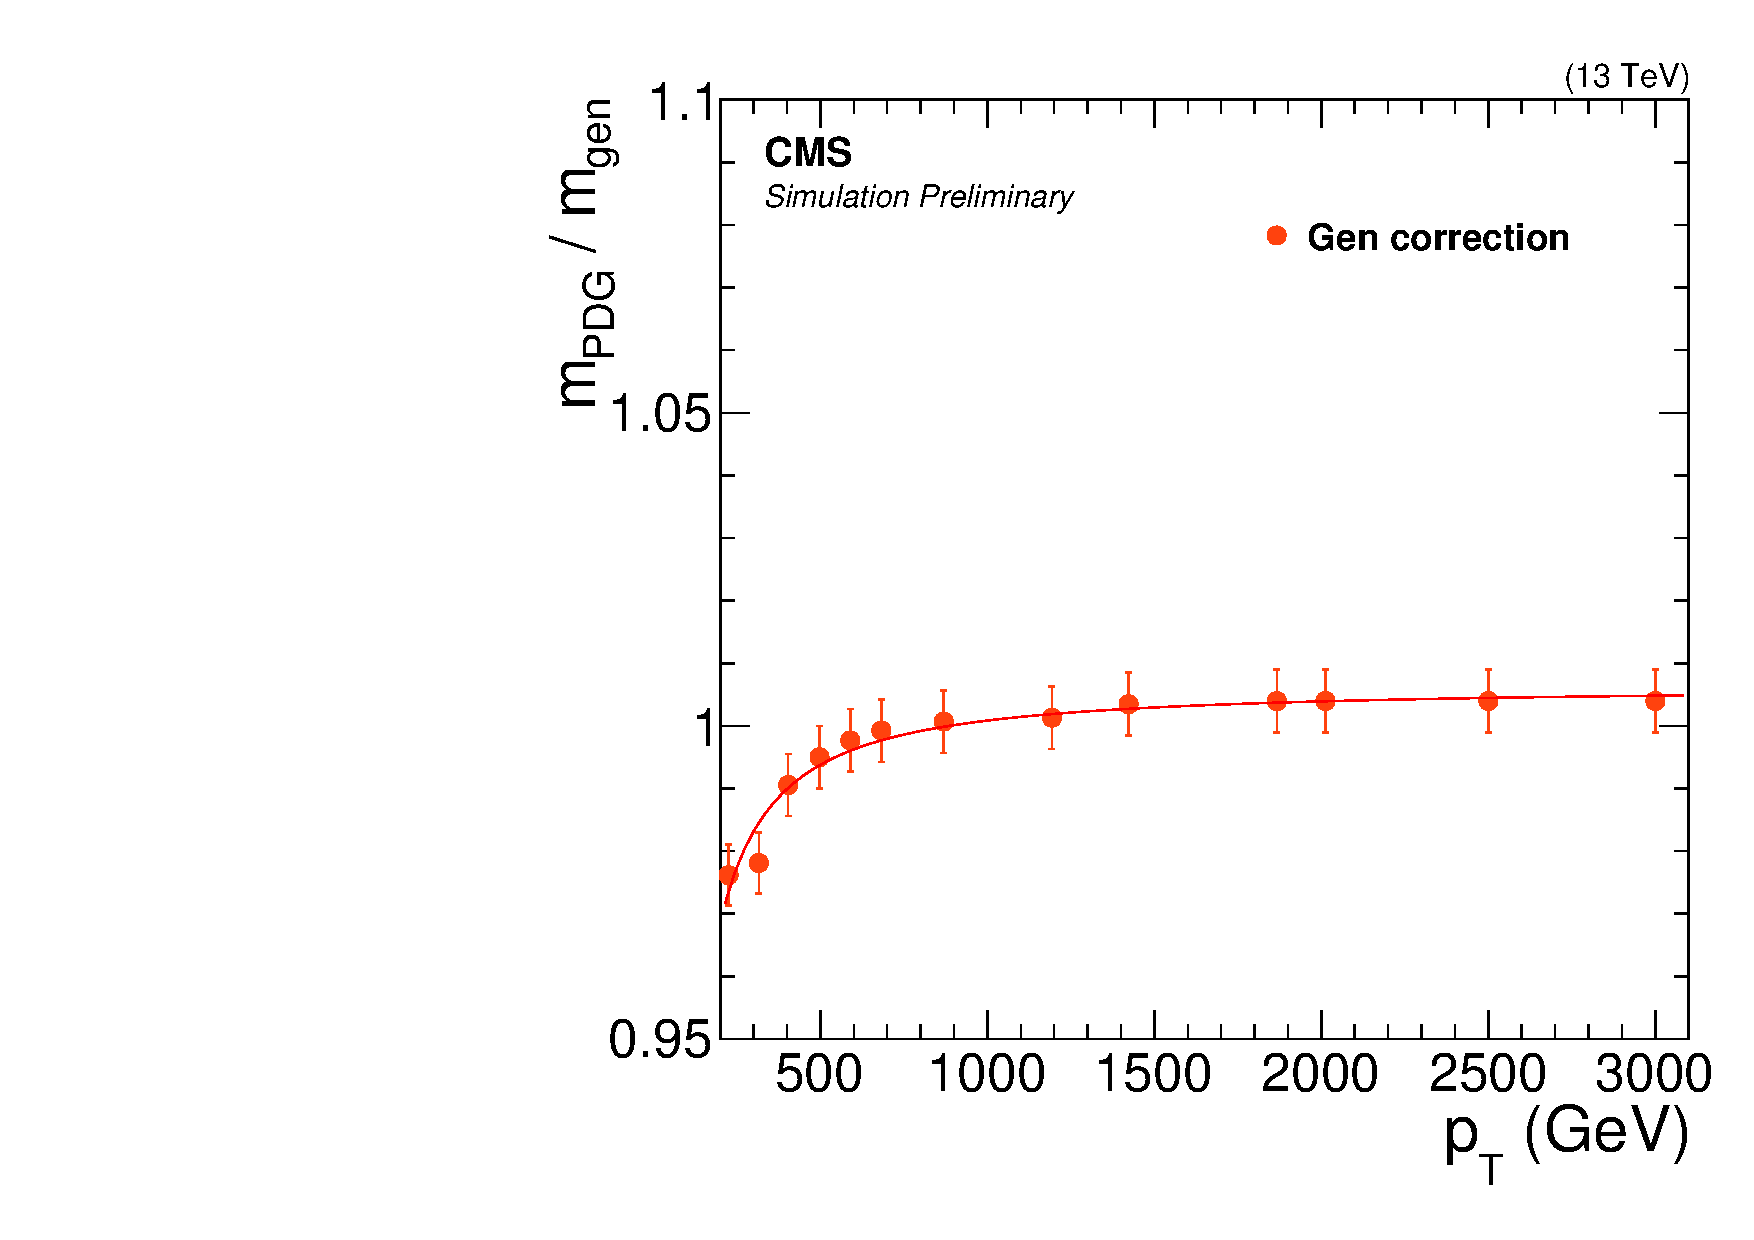
\includegraphics[width=0.45\textwidth]{figures/analysis/search2/AN-16-235/plots/JMC_fit_gen.pdf}
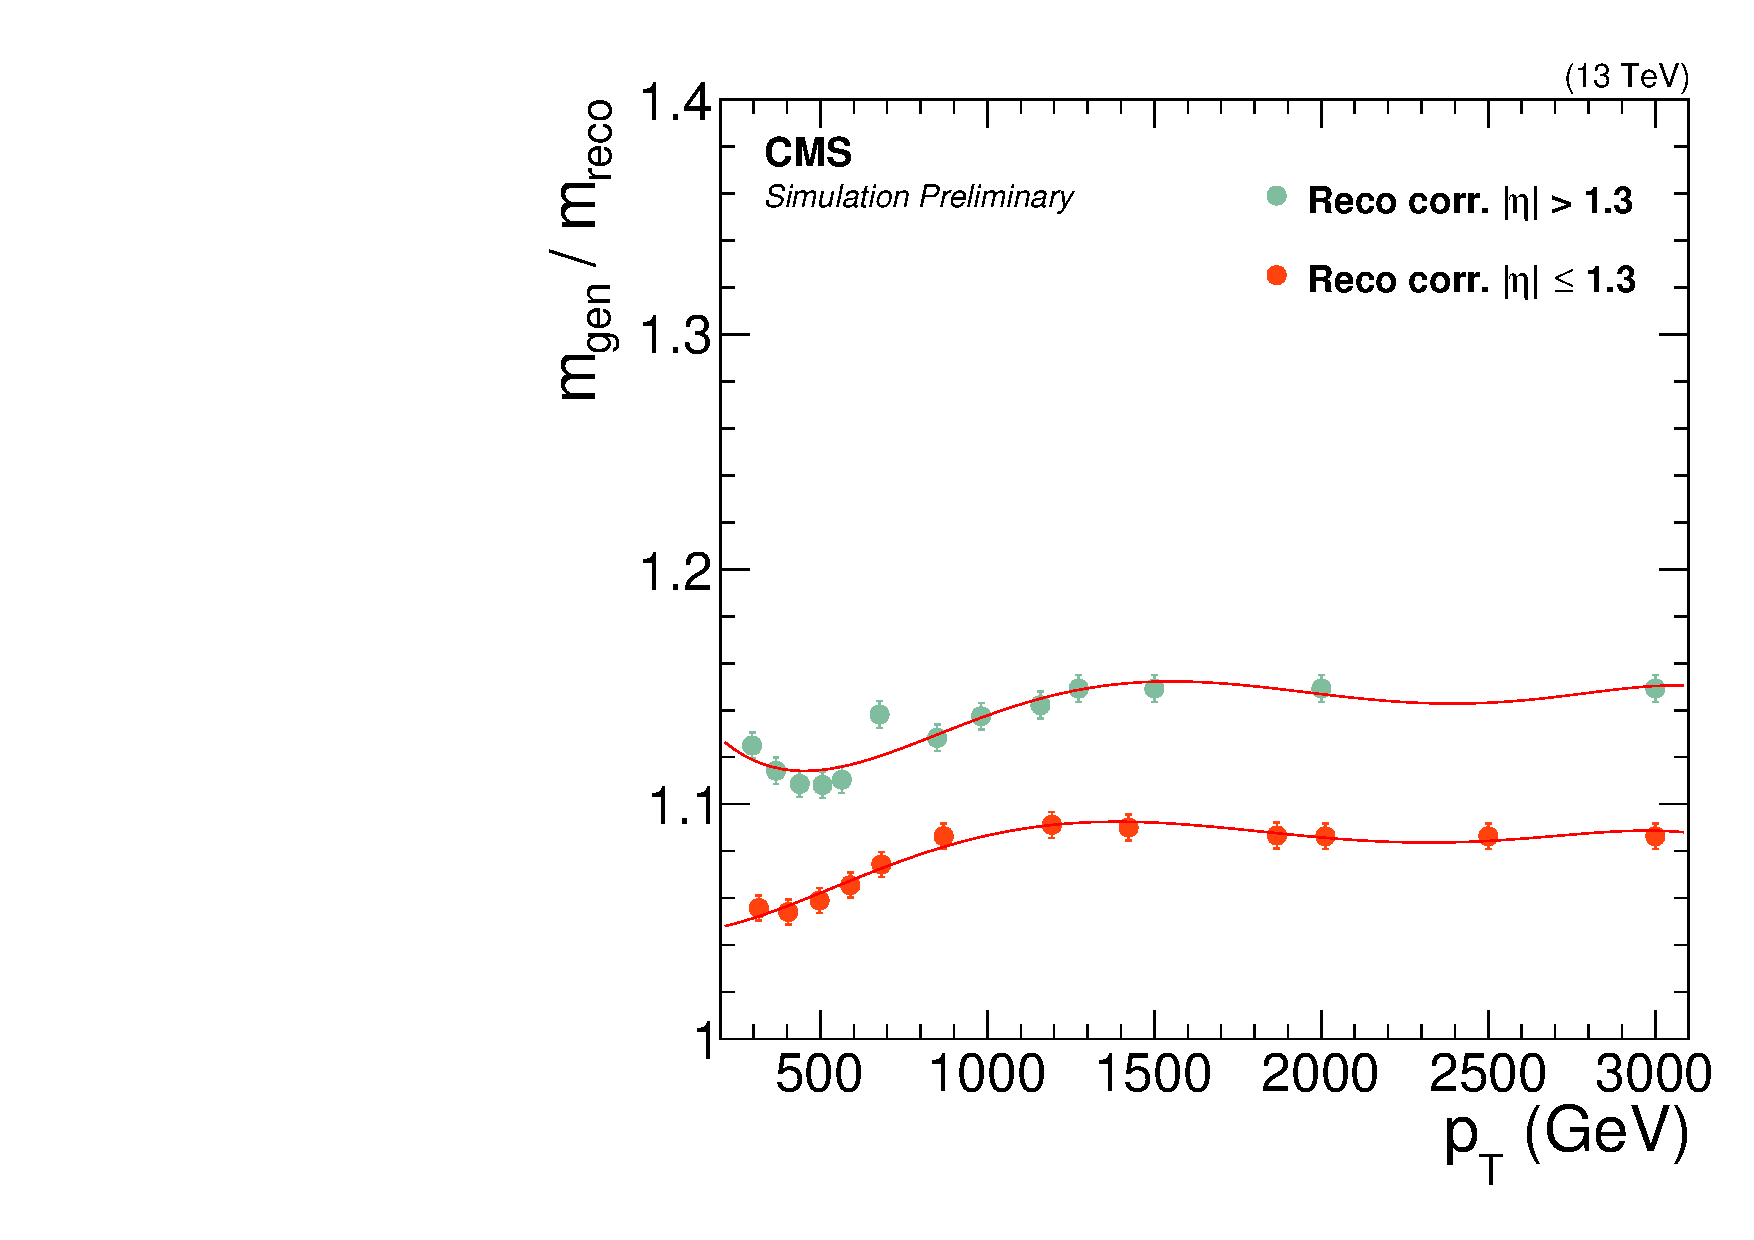
\includegraphics[width=0.45\textwidth]{figures/analysis/search2/AN-16-235/plots/JMC_fit_reco.pdf}
\caption{Fit to $\rm{M_{PDG}/M_{GEN}}$ as a function of jet $\pt$ (left), where $\rm{M_{PDG}}=80.4~\GeV$ and $\rm{M_{GEN}}$ is the fitted mean of the generator level mass and a fit to $\rm{(M_{RECO}-M_{GEN})/M_{RECO}}$ (right), where $\rm{M_{RECO}}$ is the reconstructed softdrop mass, as a function of jet $\pt$ in two $\eta$ bins.}
\label{fig:jmcfits}
\end{figure}
The two corrections are then applied to the uncorrected PUPPI softdrop mass both in data and in MC as
\begin{equation}
M_{SD}=M_{\rm{SD, uncorr}} \times \rm{w_{GEN}} \times \rm{w_{RECO}}
\end{equation}
where $w_{GEN}$ and $w_{RECO}$ correspond to the gen and reco corrections respectively and $M_{\rm{SD, uncorr}}$ is the uncorrected PUPPI softdrop mass. \par
Finally, a closure test is performed in order to check that the corrected PUPPI+softdrop W-jet mass peaks at 80.4 \GeV and is stable with \PT and $\eta$. The fitted mean of the corrected PUPPI softdrop mass peak as a function of jet \PT in two different $\eta$ bins is shown in Figure~\ref{fig:searchII:wtagclosure}. Good closure is observed, with the corrected mass peaking around 80 GeV independent of the jet $\pt$ and $\eta$.The PUPPI softdrop jet mass peak for W/Z-jets from different signal samples after jet mass corrections have been applied is shown in Figure~\ref{fig:search2:corrMass}, for resonances with a mass of 1 and 4 TeV. The corrections applied to Z-jets yield a mass stable with \PT, peaking around the Z mass. 
\begin{figure}[htbp]
\centering
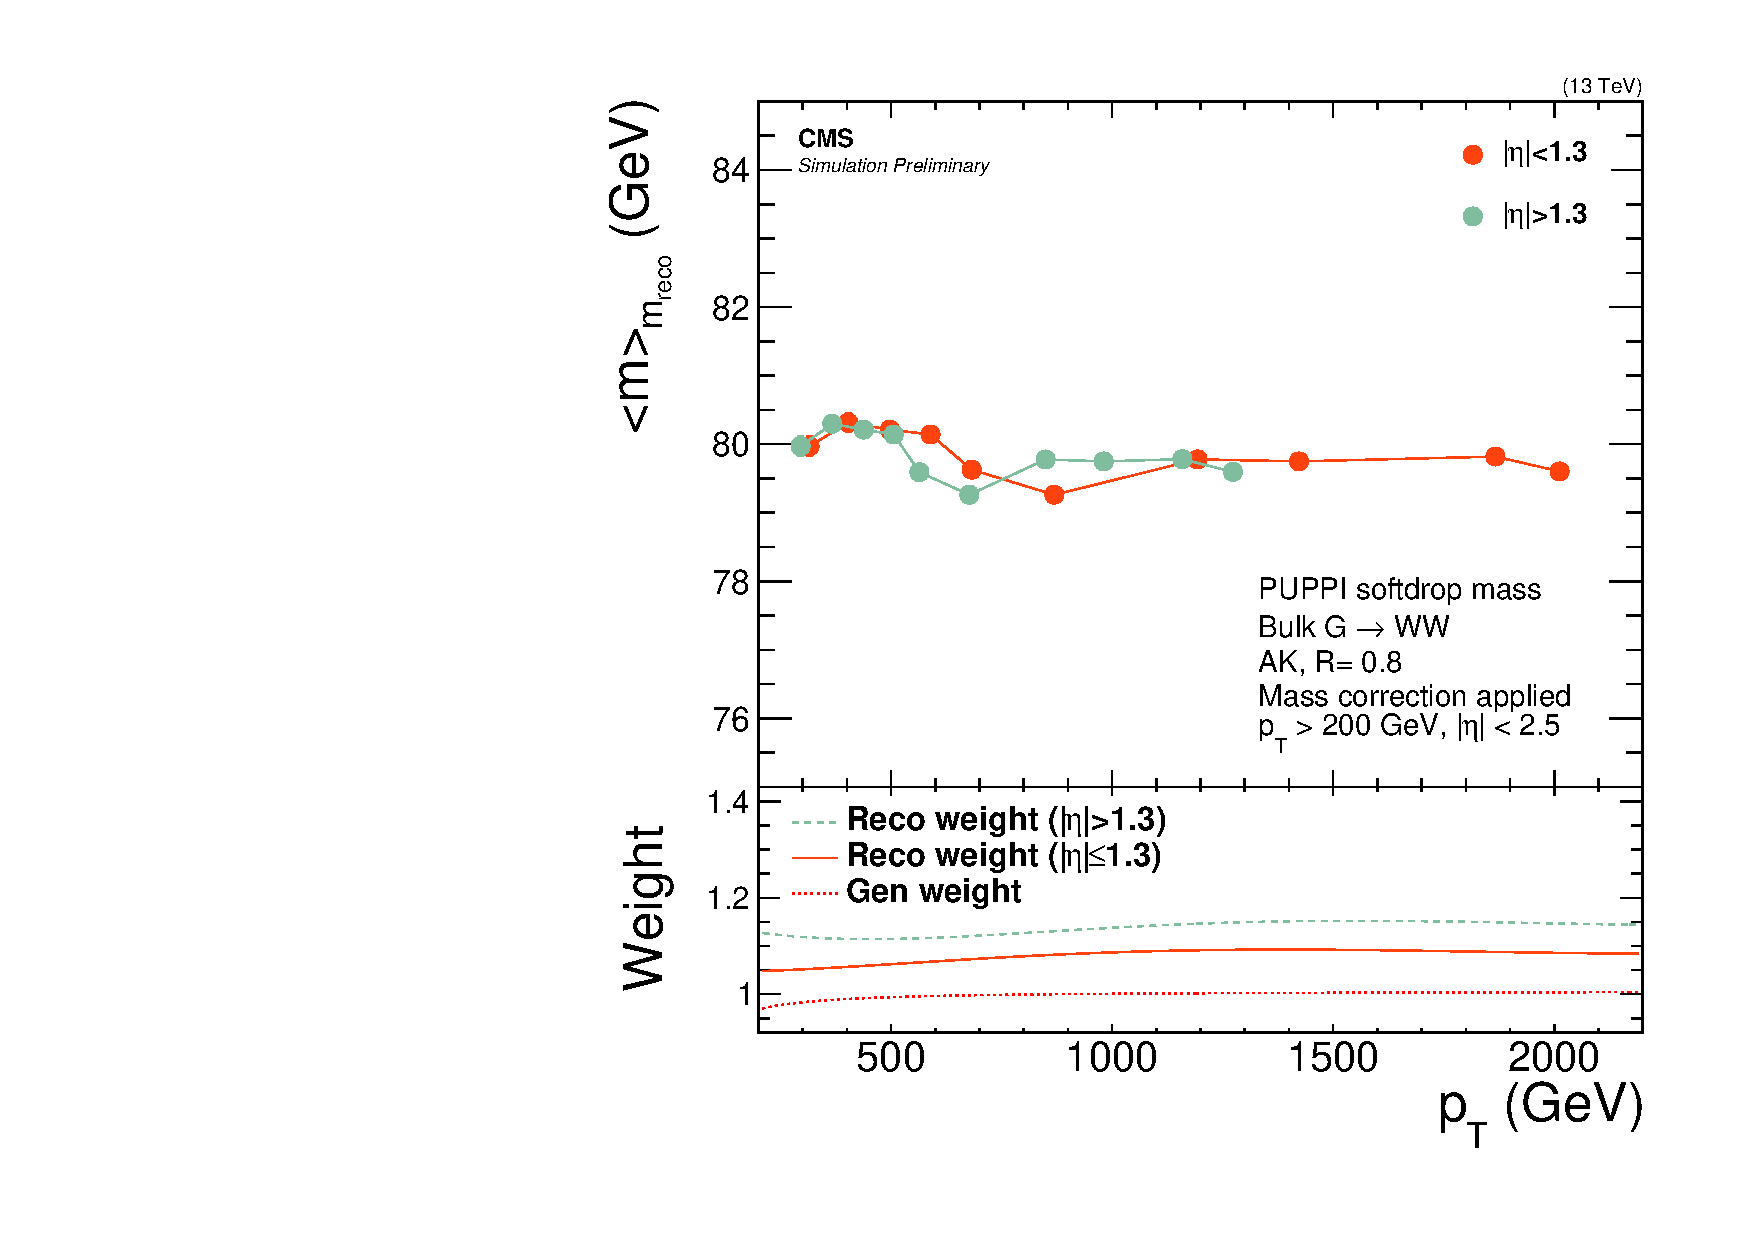
\includegraphics[width=0.49\textwidth]{figures/analysis/search2/AN-16-235/plots/ClosureTest_RecoMass.pdf}
\caption{The mean of the fitted W-jet corrected PUPPI softdrop mass peak as a function of jet $\pt$ in two different $\eta$ bins.}
\label{fig:searchII:wtagclosure}
\end{figure}
\begin{figure}[htbp]
\centering
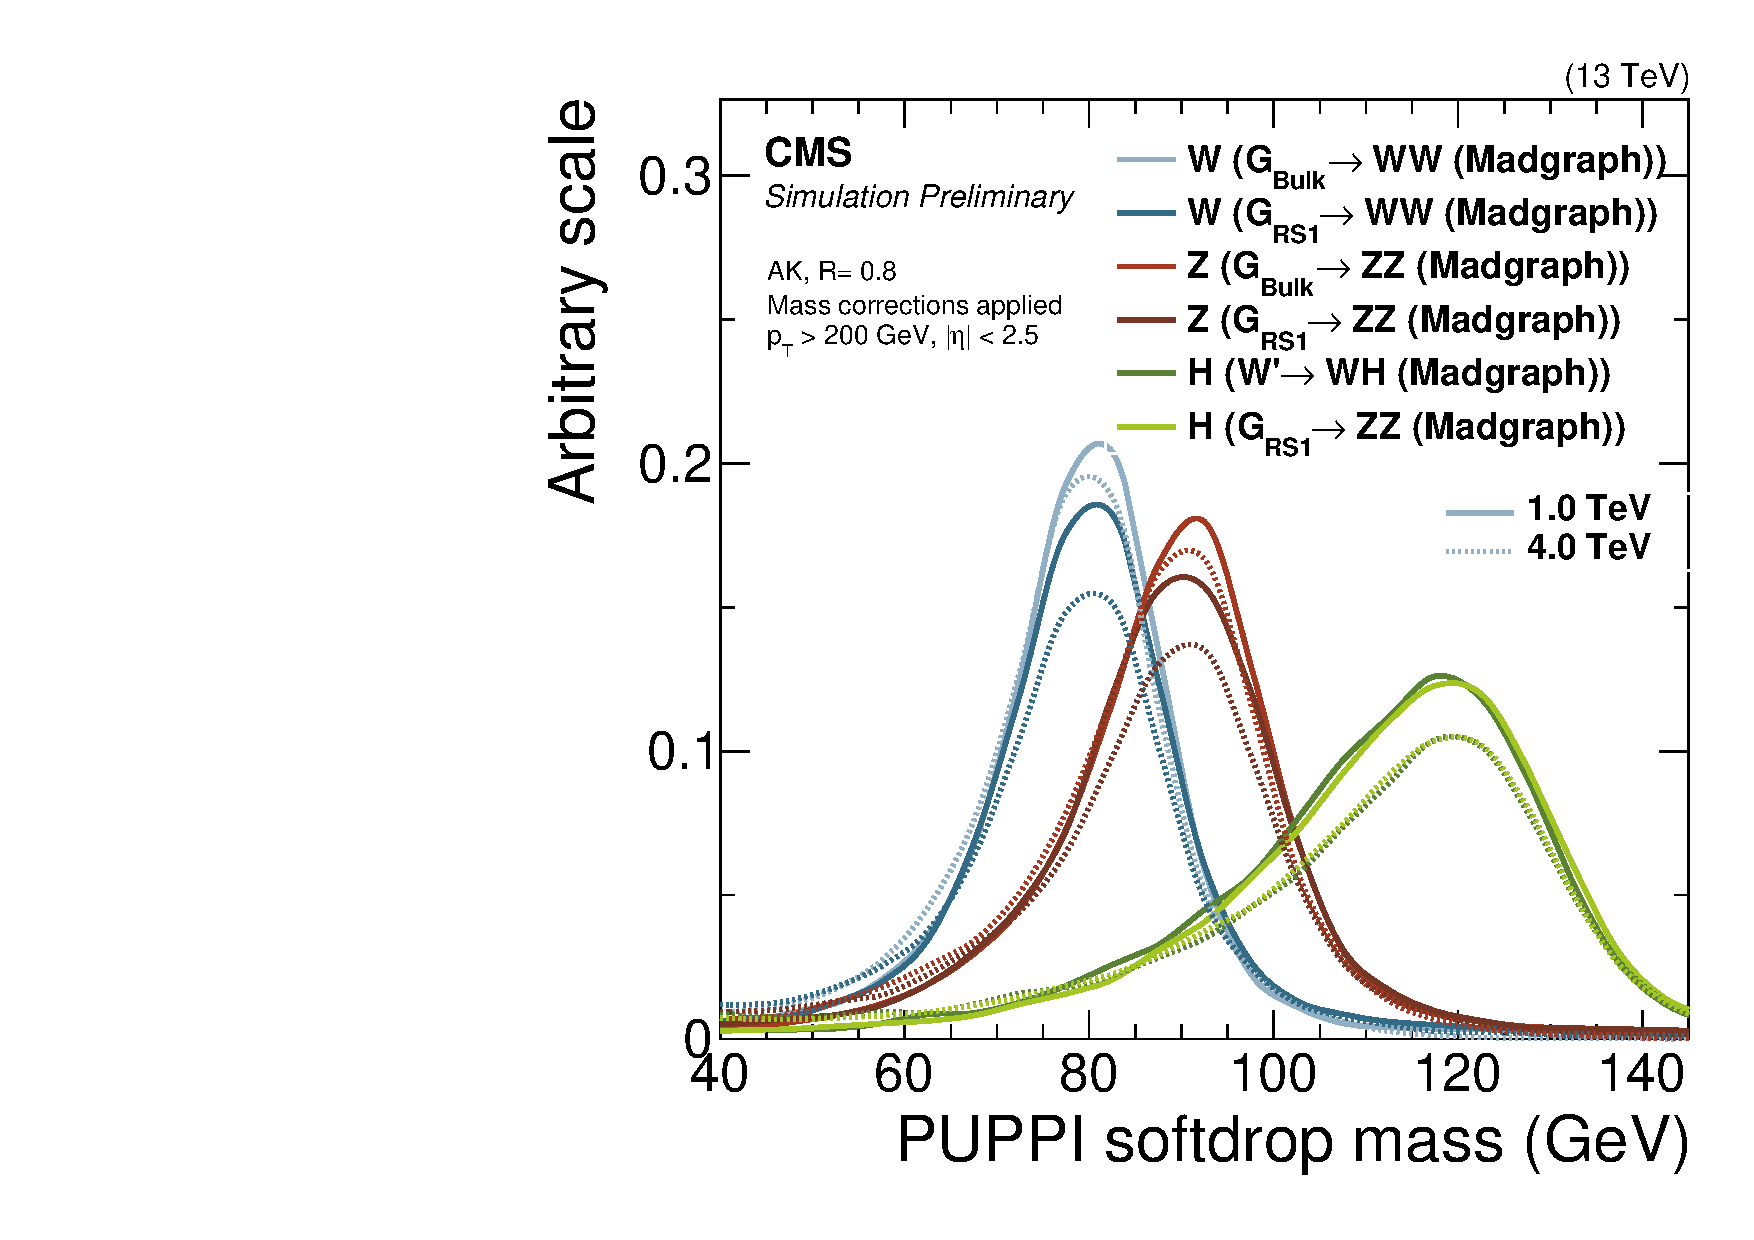
\includegraphics[width=0.49\textwidth]{figures/analysis/search2/AN-16-235/plots/SoftdropMass_NEWCORR_wH0.pdf}
\caption{The W/Z/H-jet corrected PUPPI softdrop mass peak for jets from different signal samples with masses of 1 and 4 TeV.}
\label{fig:search2:corrMass}
\end{figure}

\subsubsection{W-tagging performance}
The new PUPPI+softdrop based \PW/\PZ-tagger uses a mass window of $65 \GeV < m_{SD} < 105 \GeV$ in combination with a cut of PUPPI $\tau_{21}<0.4$.
We compare its performance to that of the CHS+pruning based tagger used in Search I as well as to that of a "DDT-transformed" \nsubj based tagger~\cite{Dolen:2016kst}. The $\tau_{21}^{DDT}$ variable is a linear transformation of \nsubj given as
\begin{equation}
\tau_{21}^{DDT} = \tau_{21} + M \times \log \bigg( \frac{m^2}{p_T \times 1 \textrm{ GeV}}\bigg)
\end{equation}
where $M=-0.063$ is obtained from a fit of $\tau_{21}$ against the variable $\rho^{'}=\log(m^2/\PT/\mu)$, where $\mu = 1 \GeV$.
The purpose of this is to decorrelate $\tau_{21}$ from the softdrop mass and \PT, yielding a mass and dijet invariant mass spectrum minimally sculpted by
a cut on the $\tau_{21}^{DDT}$ tagging variable. This is tagger that will be further explored and explained in detail in the context of Search III, Section~\ref{sec:searchIII:ddt}.\par
The background rejection efficiency for QCD light flavor jets as a function of W-jet signal efficiency is shown in Figure~\ref{fig:searchII:roc}
The efficiency is measured requiring a fixed jet mass window of 65-105 \GeV, while scanning the cut on $\tau_2/\tau_1$.
\begin{figure}[ht!]
\centering
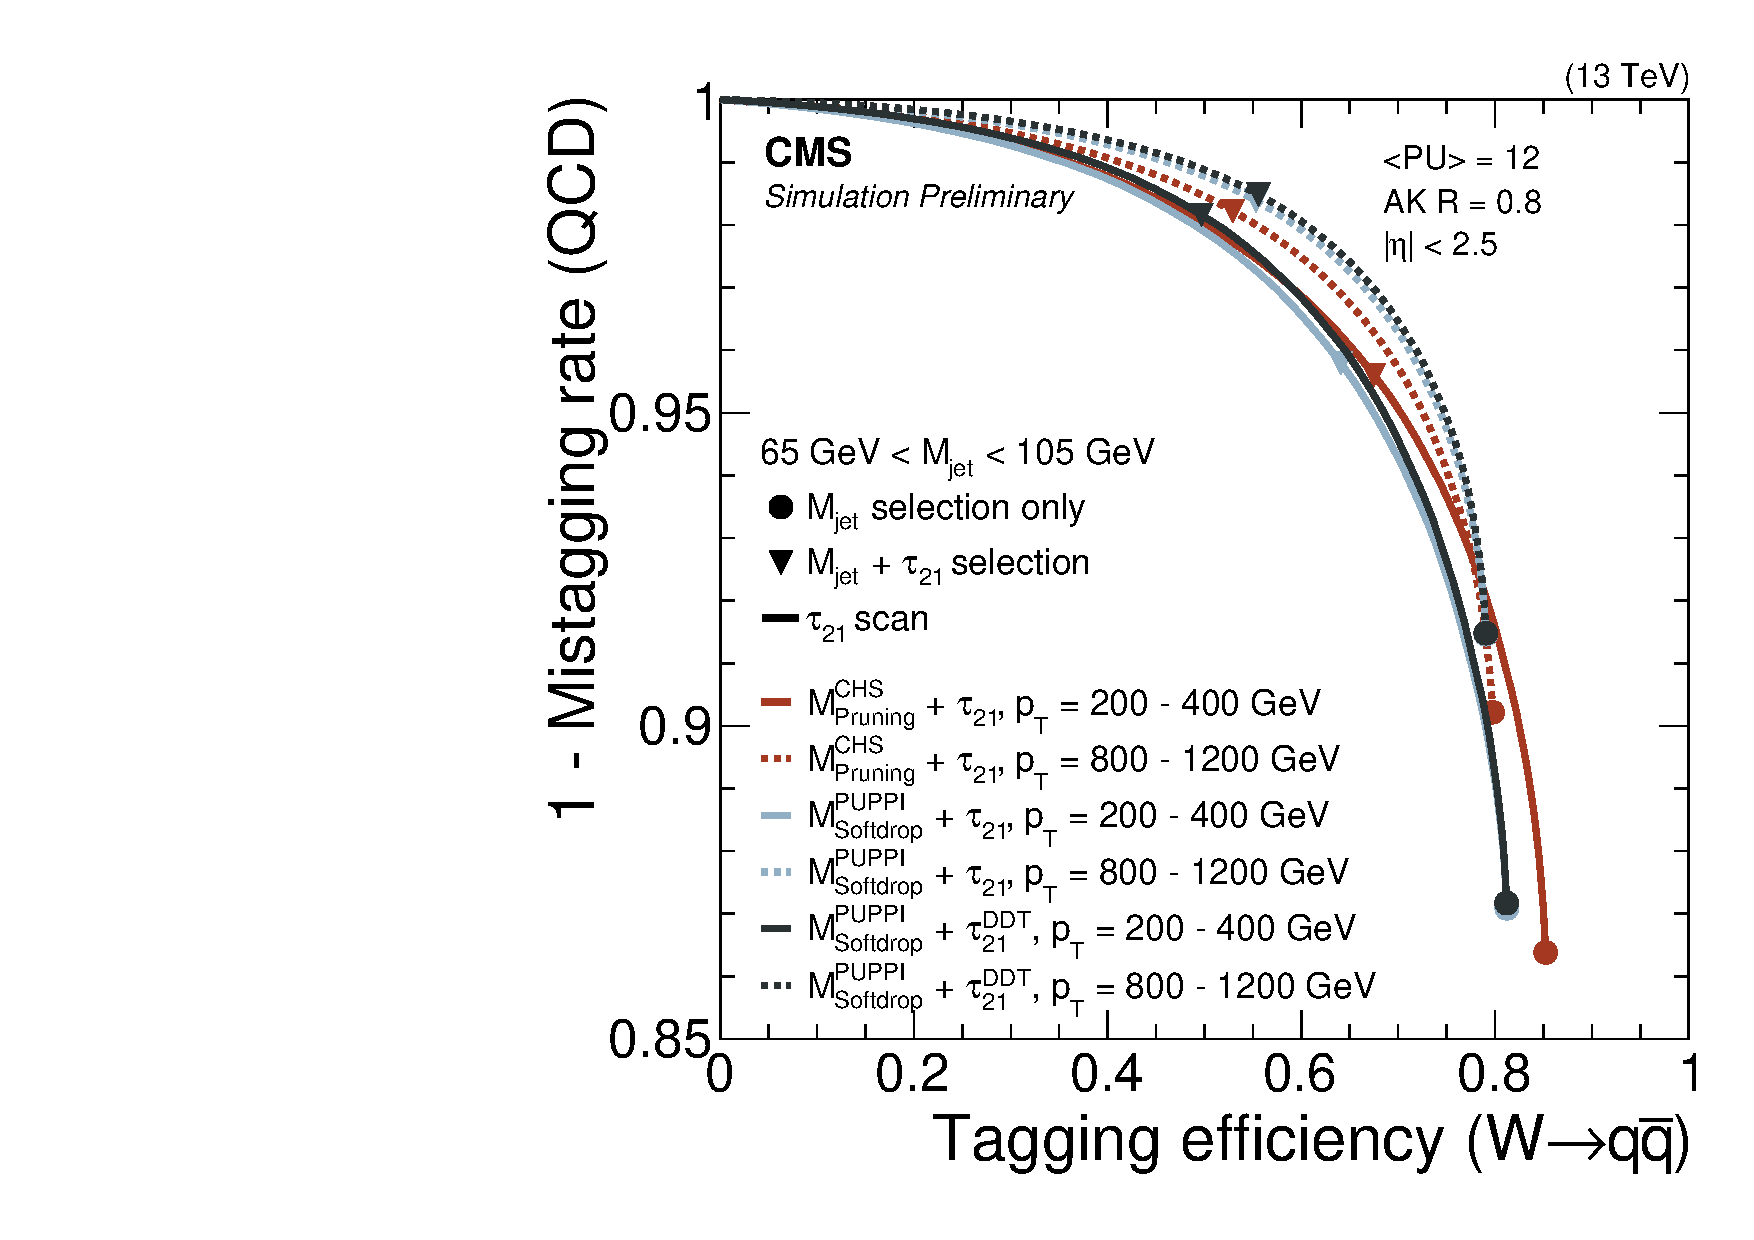
\includegraphics[width=0.49\textwidth]{figures/vtagging/JME-16-003/BoostedW/roc_WqqvsQCD_2bins.pdf}
\caption{The background rejection efficiency for QCD light flavor jets as a function of W-jet signal efficiency. A cut on CHS pruned or PUPPI softdrop jet
mass of $65<m_{\mathrm{jet}}<105$~\GeV is applied while scanning the cut on \nsubj. The cuts corresponding to $\tau_2/\tau_1 < 0.45$ for CHS+pruning, PUPPI $\tau_2/\tau_1 < 0.4$ for PUPPI+softdrop or $\tau_{21}^\text{DDT}<0.52$ are indicated with triangles, while the solid circles represent the efficiency and mistag rate for a mass cut only.}
\label{fig:searchII:roc}
\end{figure}
The general performance of each tagger is very similar, with the PUPPI+softdrop based taggers displaying a slightly higher signal efficiency for a given mistag rate at high \PT and CHS+pruning slightly better at low \PT.
Two better understand the difference between each tagger, we look at the tagging performance as a function of jet \PT as well as pileup, shown in Figure~\ref{fig:searchII:effvspt} and~\ref{fig:searchII:effvspu}.\par
Starting with the tagger \PT-dependence in Figure~\ref{fig:searchII:effvspt}, we observe that she signal efficiency of a PUPPI+softdrop of CHS+pruned jet mass cut is flat as a function of \PT, at around 80\%. The QCD mistagging rate drops for both groomers, with a 1-3\% lower mistag rate using PUPPI+softdrop that CHS+pruning.
\begin{figure}[h!]
\centering
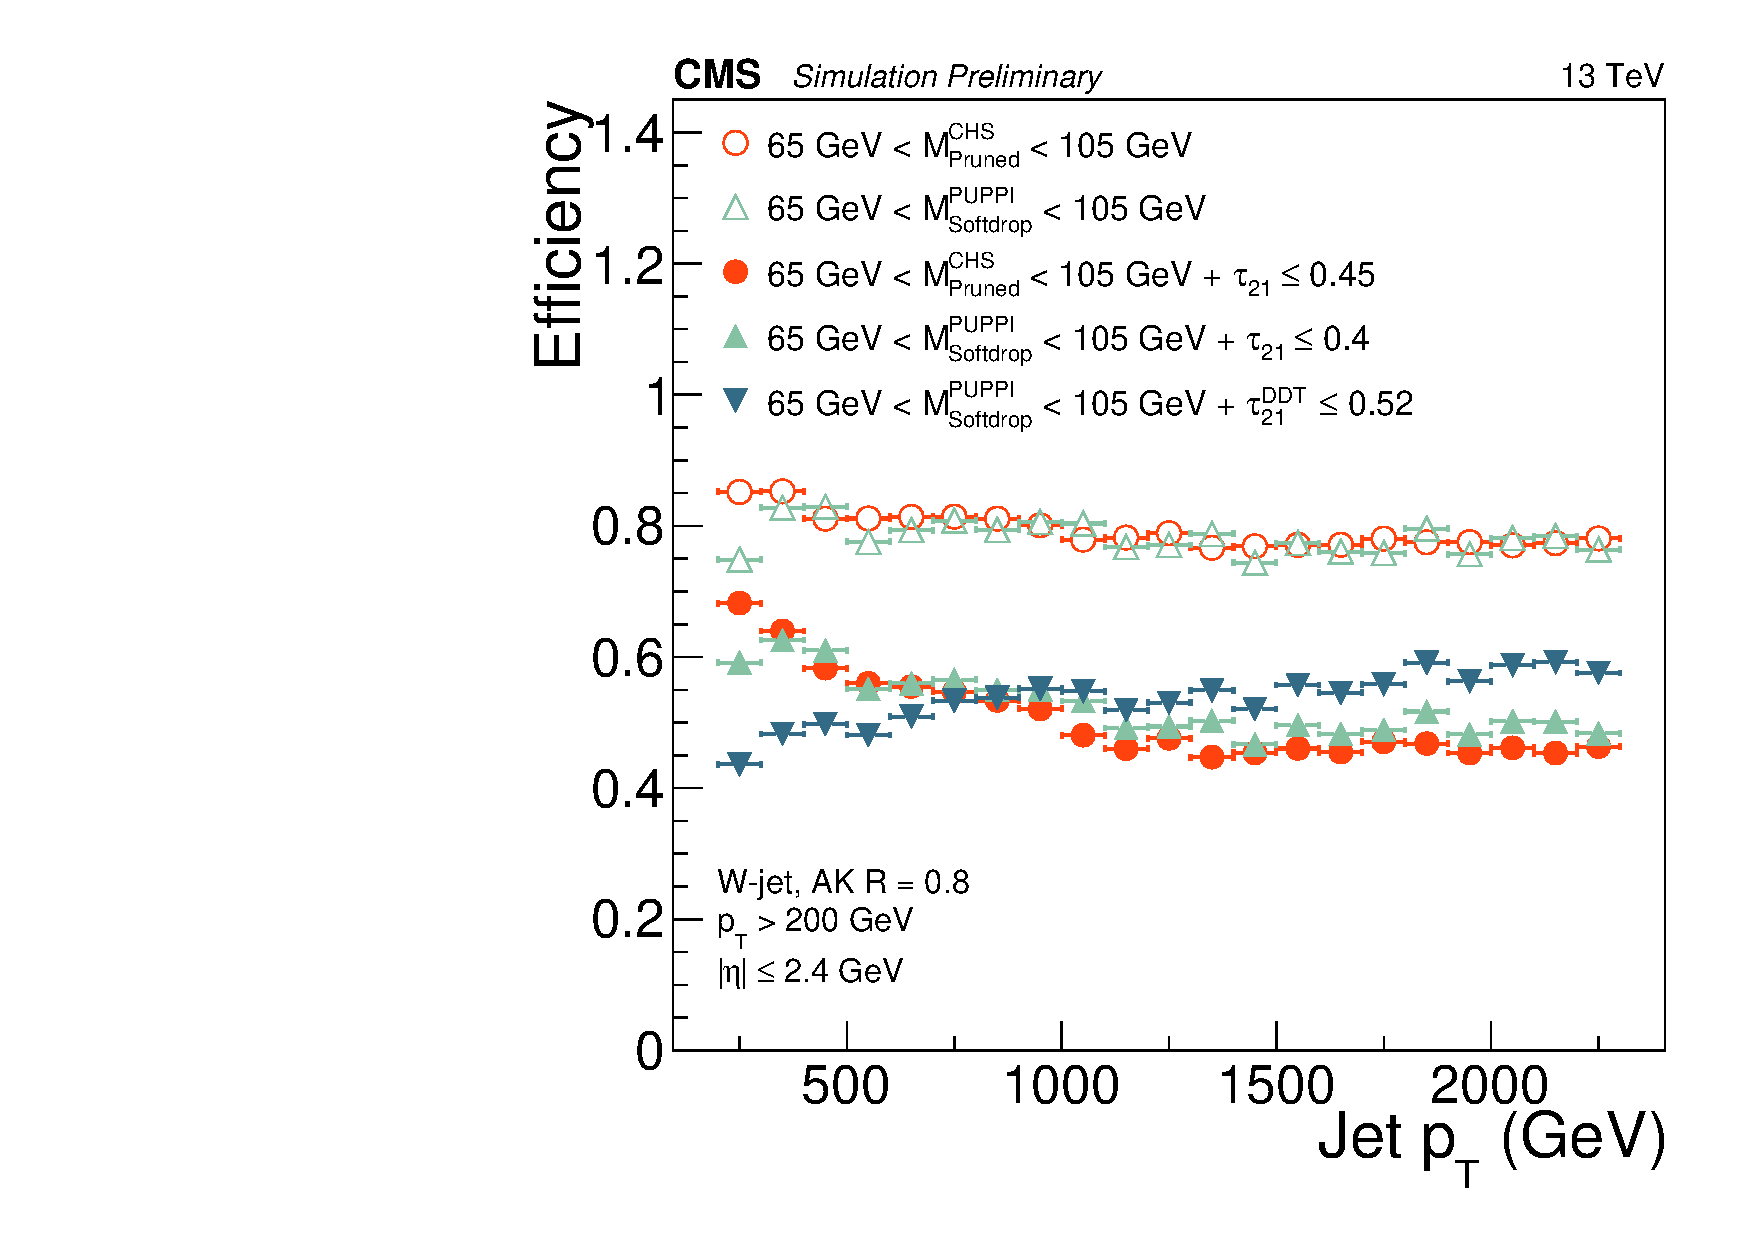
\includegraphics[width=0.49\textwidth]{figures/vtagging/JME-16-003/BoostedW/WtagSigEffvsPT.pdf}
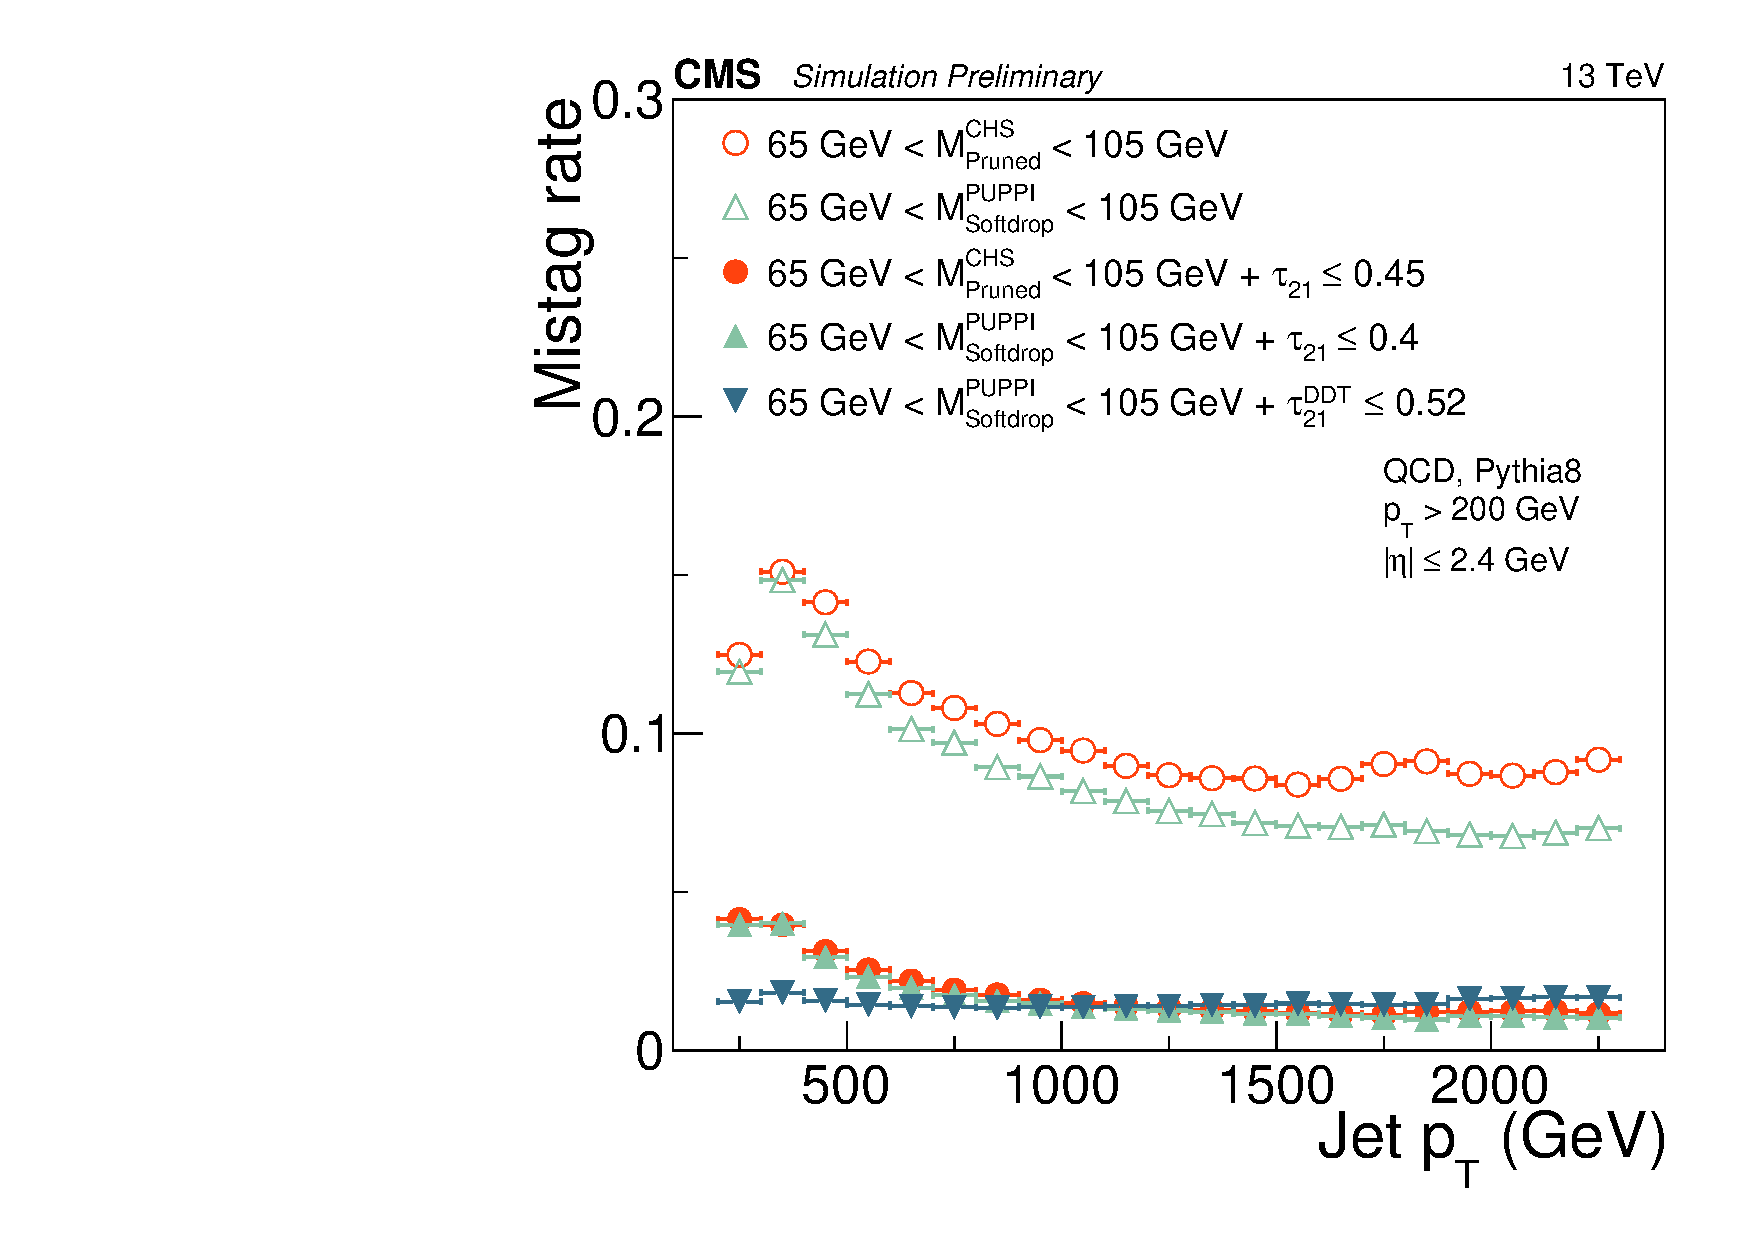
\includegraphics[width=0.49\textwidth]{figures/vtagging/JME-16-003/BoostedW/QCDBkgEffvsPT.pdf}
\caption{W-jet efficiency (left) and QCD light jet mistag rate (right) for a PUPPI+softdrop or CHS+pruned jet mass selection only (hollow circles) and the combined $m_{\mathrm{jet}}$ + (PUPPI) $\tau_2/\tau_1$ (DDT) selection (solid circles) as a function of jet \PT.}
\label{fig:searchII:effvspt}
\end{figure}
Once applying an n-subjettiness cut, the signal efficiency as well as the mistag rate for the PUPPI \nsubj and CHS \nsubj taggers drops as a function of \PT, with an average signal efficiency of around 50\% for a $\sim 2\%$ mistag rate. An interesting behavior is observed for the $\tau_{21}^{DDT}$ tagger: While the mistag rate is flat as a function of \PT, as is the purpose of decorrelated taggers, the signal efficiency improves as the \PT increases, outperforming the other taggers above 1 \TeV. \par
Turning to the tagger pileup dependence, shown in Figure~\ref{fig:searchII:effvspu}, the expected benefit from using the PUPPI algorithm is observed: The tagging efficiency for the CHS+pruning (red solid cirles) based tagger falls of steeply versus the number of primary vertices in the event, while the PUPPI+softdrop based taggers (light and dark blue solid circles) are more or less insensitive to pileup.
\begin{figure}[h!]
\centering
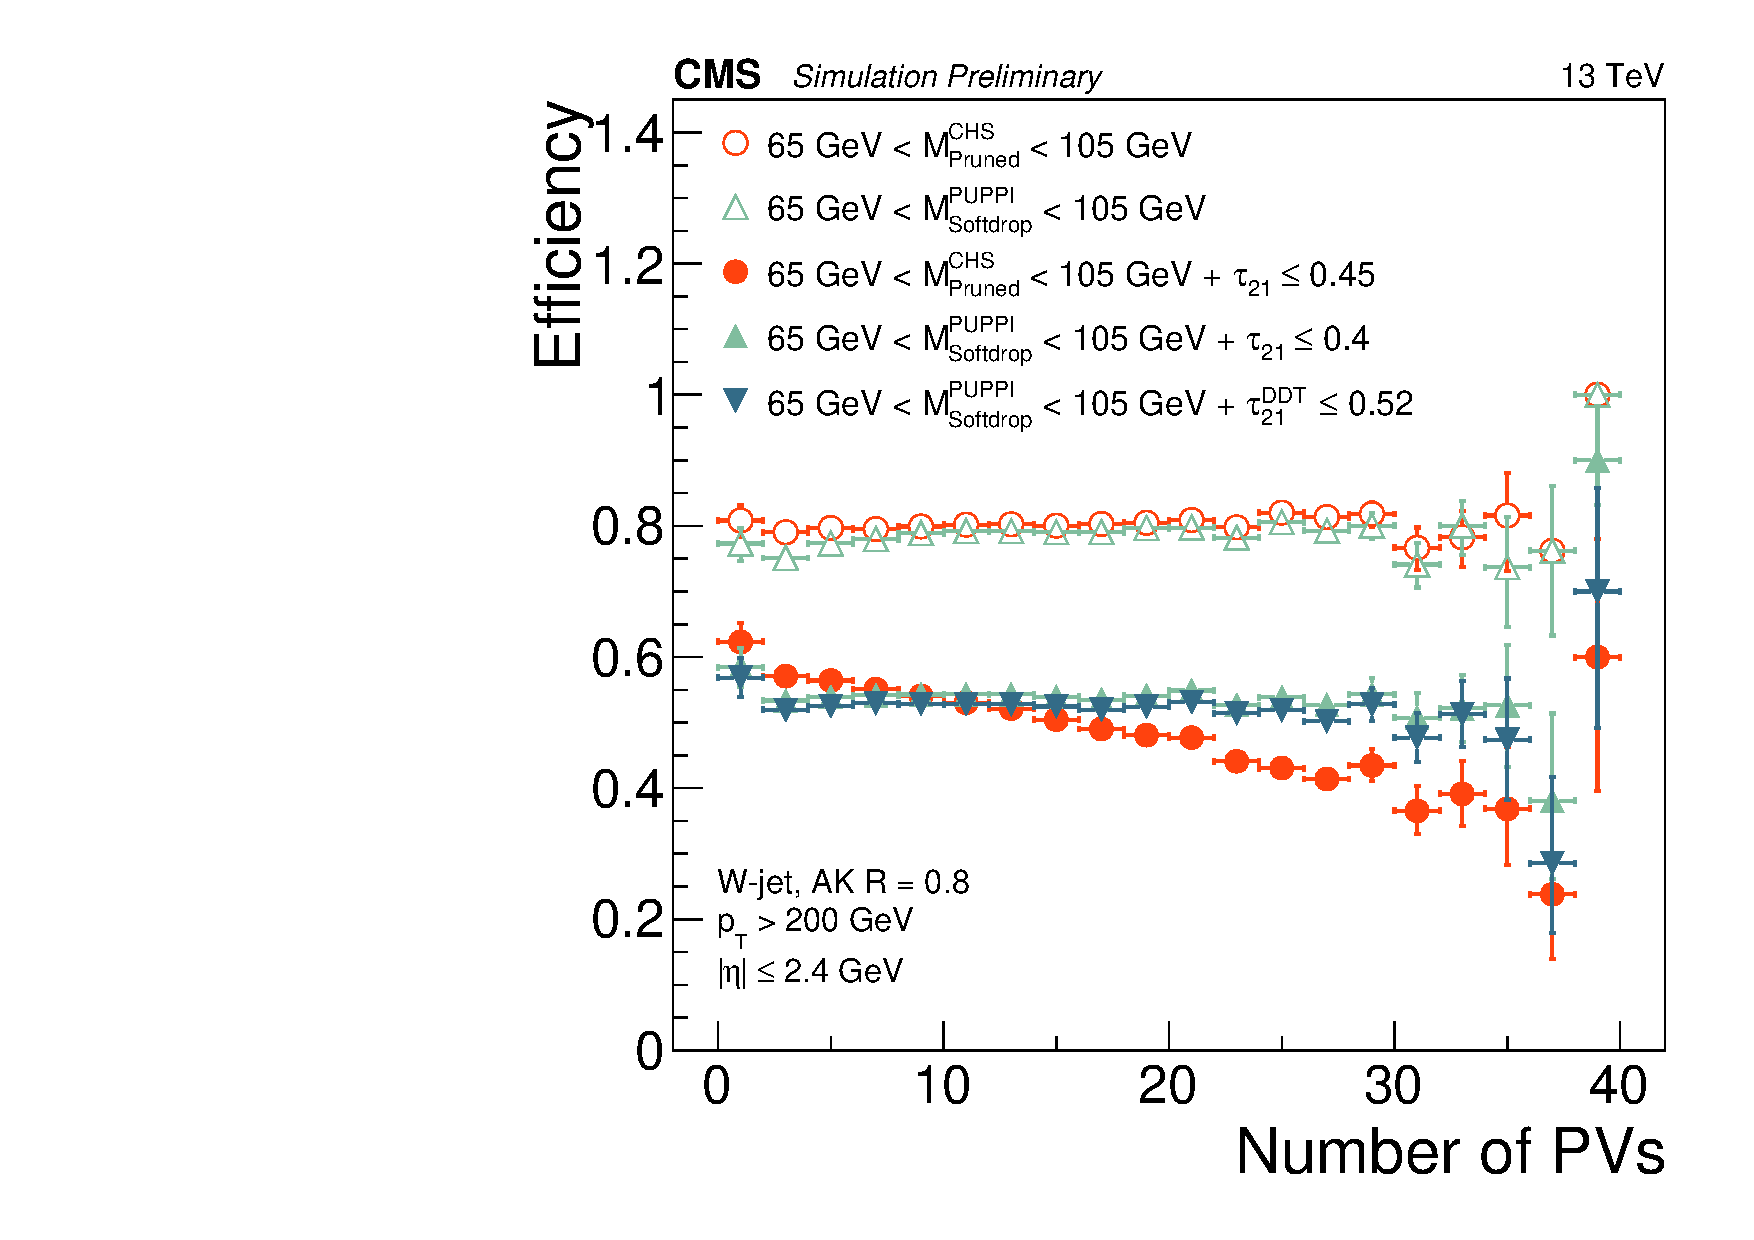
\includegraphics[width=0.49\textwidth]{figures/vtagging/JME-16-003/BoostedW/WtagSigEffvsNPV.pdf}
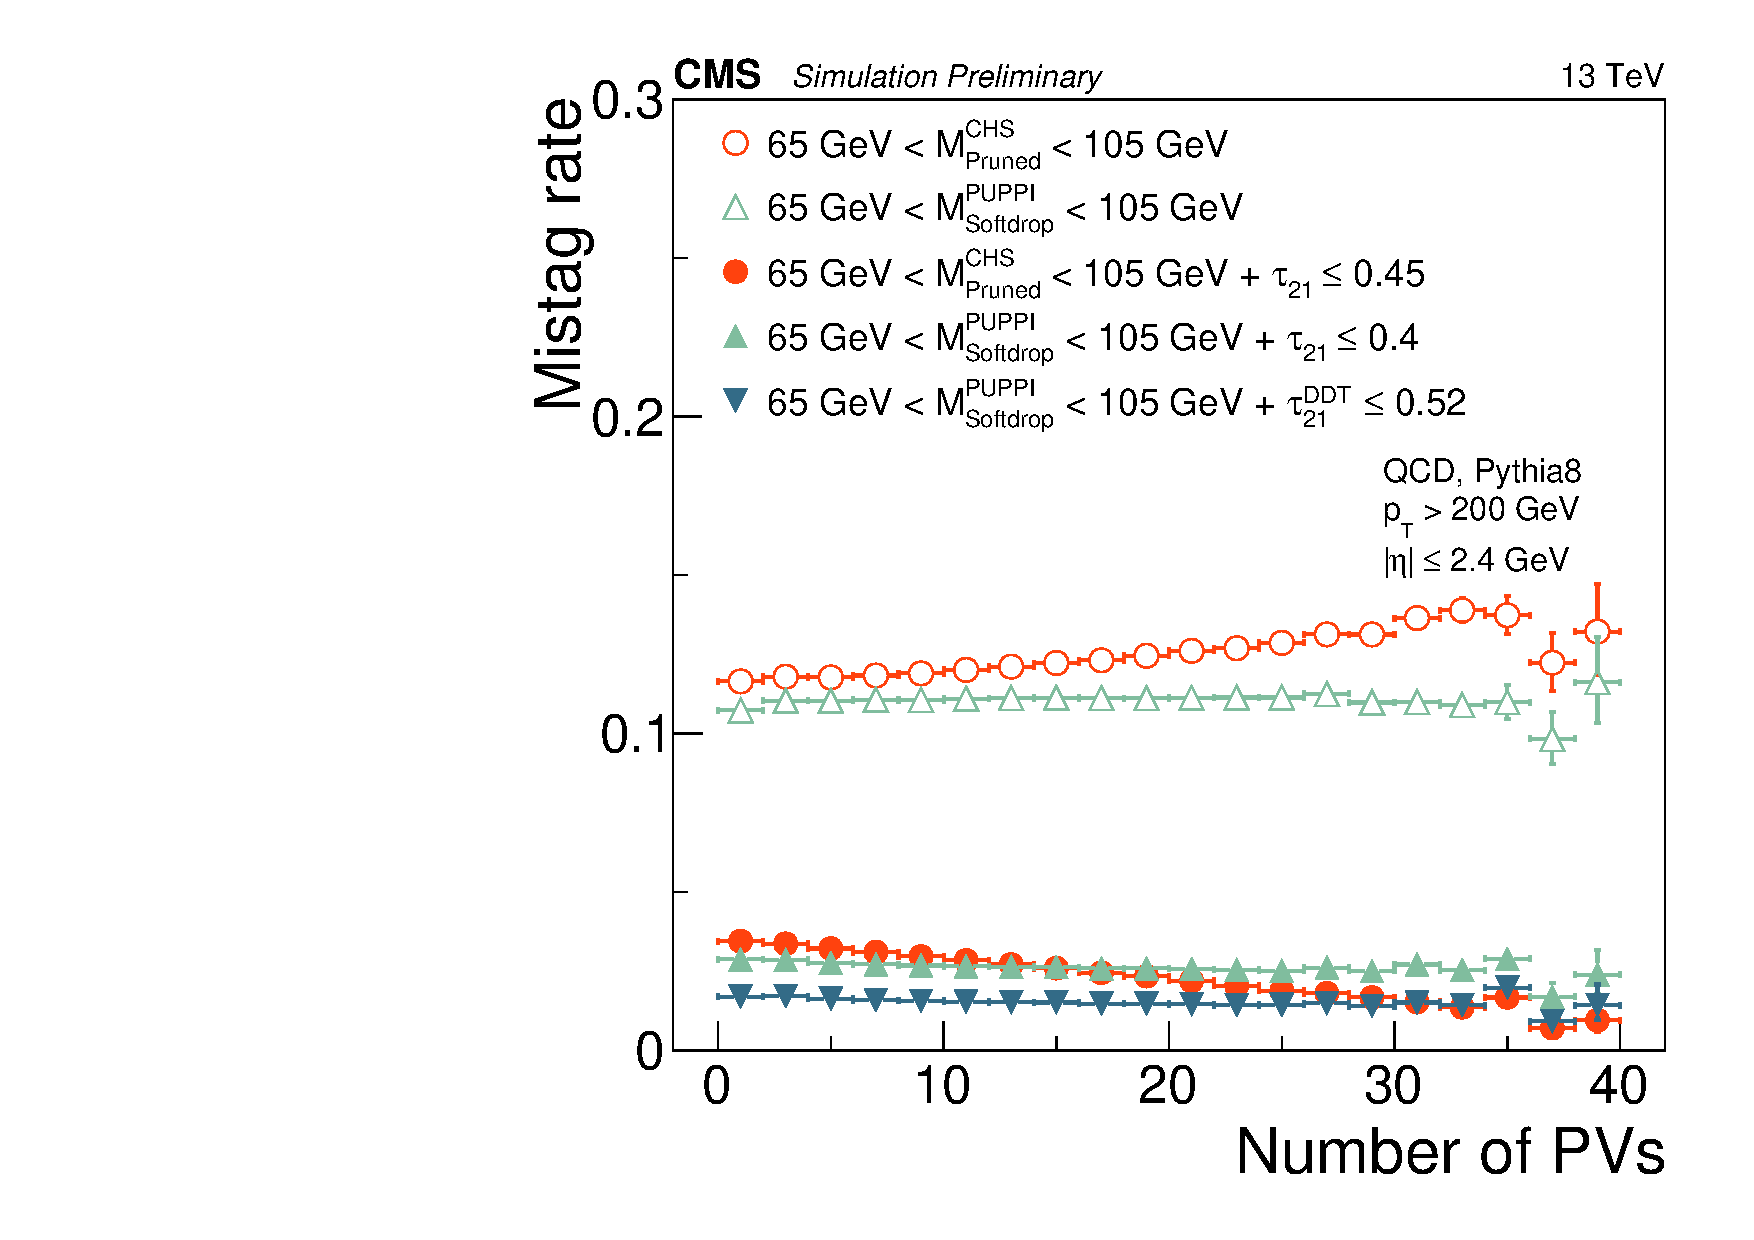
\includegraphics[width=0.49\textwidth]{figures/vtagging/JME-16-003/BoostedW/QCDBkgEffvsNPV.pdf}
\caption{W-jet efficiency (left) and QCD light jet mistag rate (right) for a PUPPI+softdrop or CHS+pruned jet mass selection only (hollow circles) and the combined $m_{\mathrm{jet}}$ + (PUPPI) $\tau_2/\tau_1$ (DDT) selection (solid circles) as a function of jet pileup.}
\label{fig:searchII:effvspu}
\end{figure}
Based on general performance, tagging stability versus pileup and due to theoretical considerations, PUPPI sofdrop mass with dedicated mass corrections applied together with PUPPI \nsubj is chosen as this analysis W-tagger. The per-jet efficiency is around 50-55\% for a 1-2\% mistag rate.\par

The PUPPI softdrop jet mass and PUPPI \nsubj distribution in data is shown in Figure~\ref{fig:searchII:wtag}
We see some disagreement between data and MC, especially in the high-purity region (PUPPI $\ddt<0.4$). In order to have an accurate estimate of the signal efficiency when applying this W-tagger, a good measurement of the difference in tagging efficiency between data and MC is crucial and is what we will focus on next.
\begin{figure}[h!]
\centering
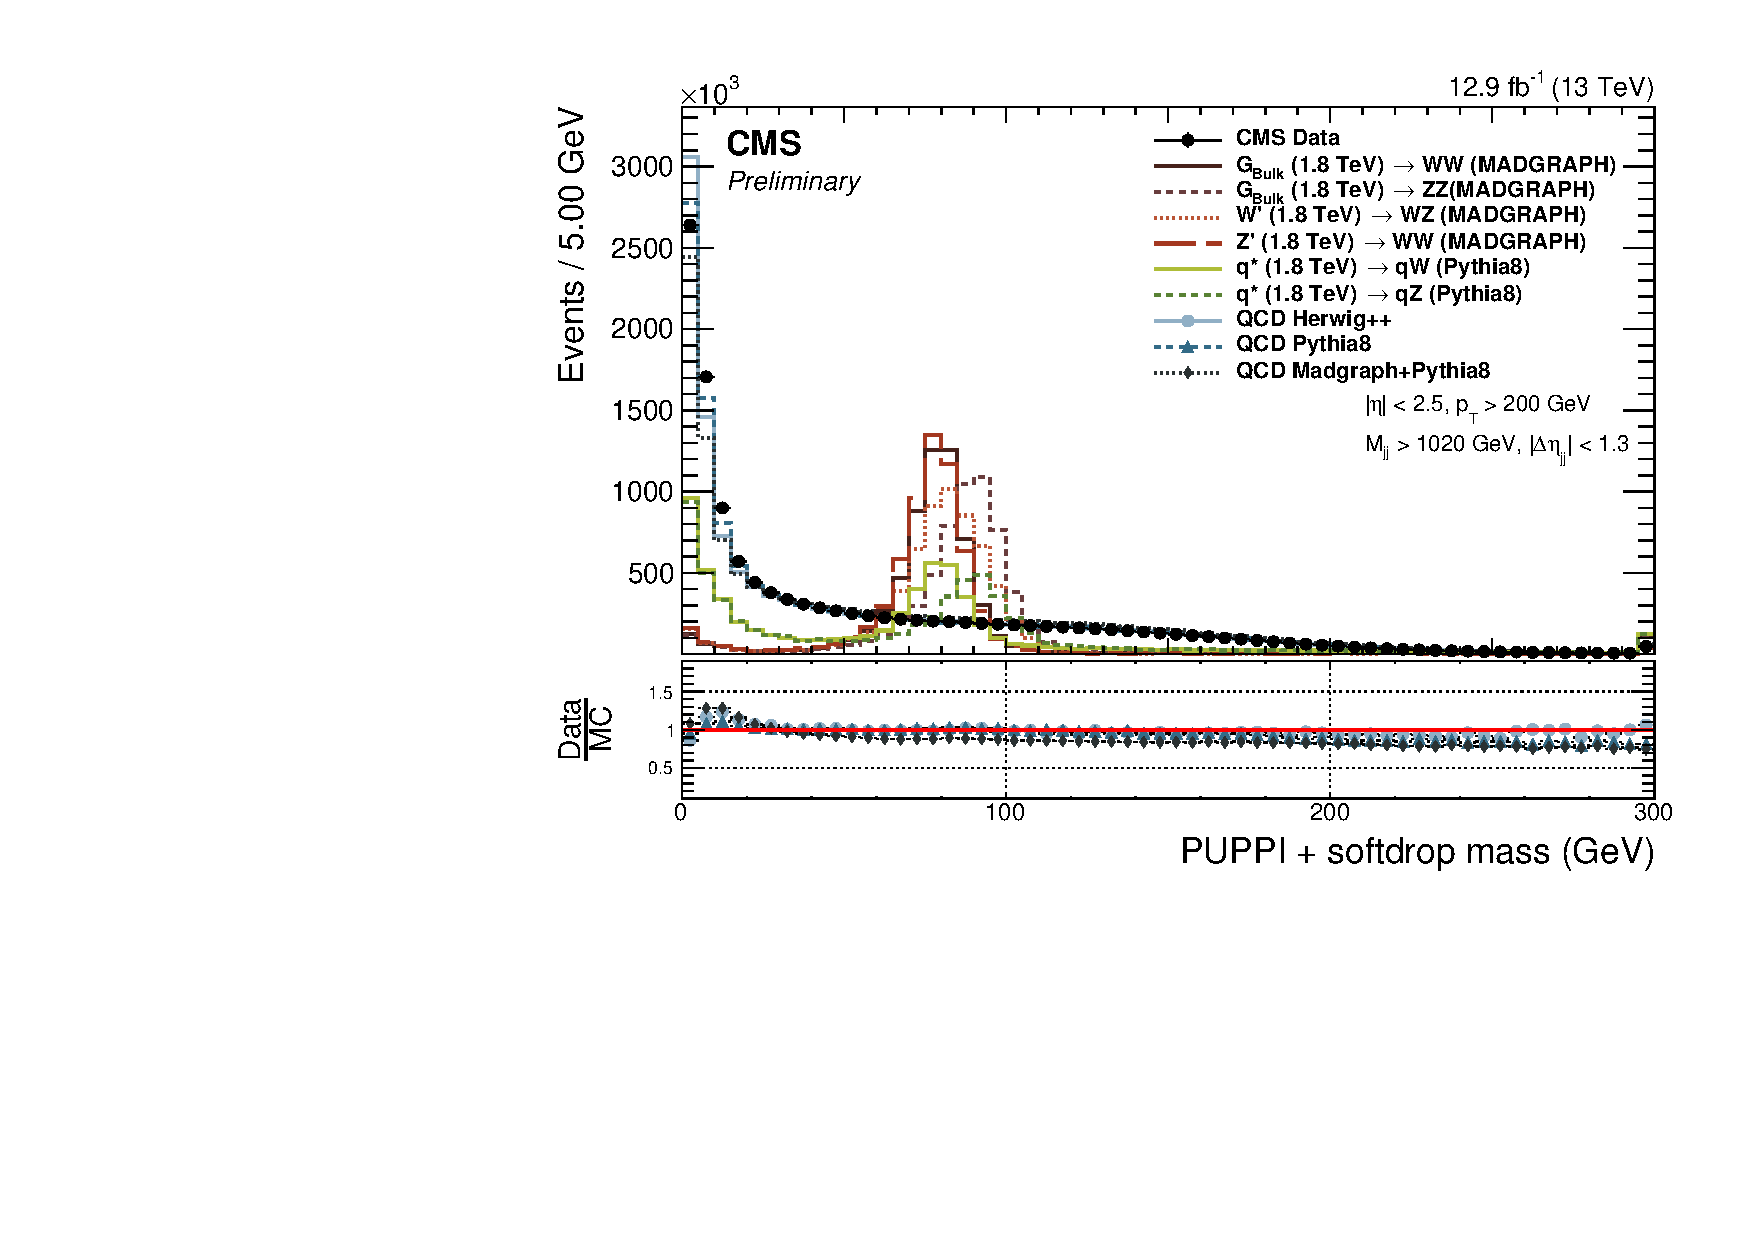
\includegraphics[width=0.49\textwidth]{figures/analysis/search2/AN-16-235/plots/qcdcp_PuppiSoftdropMass.pdf}
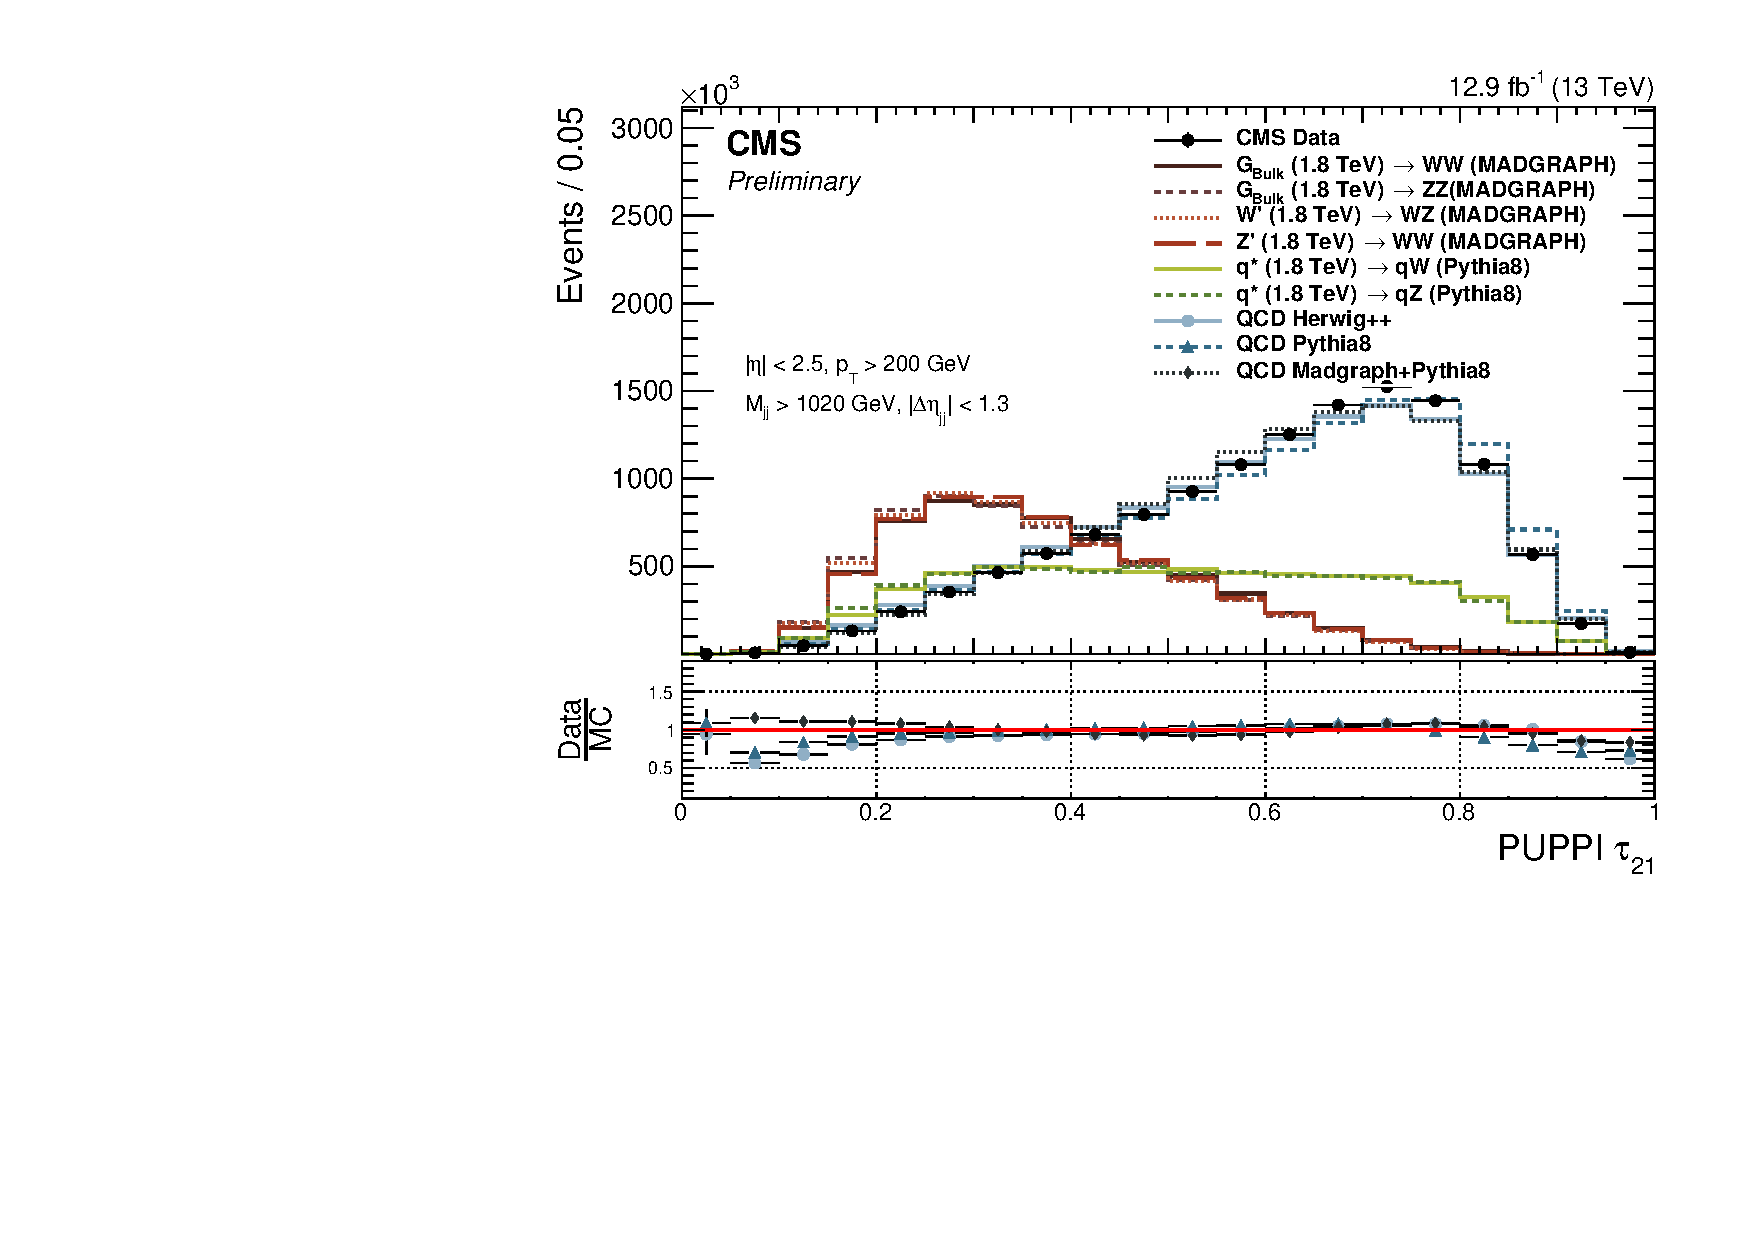
\includegraphics[width=0.49\textwidth]{figures/analysis/search2/AN-16-235/plots/qcdcp_puppi_tau2tau1.pdf}
\caption{PUPPI softdrop jet mass distribution (left) and PUPPI n-subjettiness $\tau_{21}$ (right) distribution for data and simulated samples. Simulated samples are scaled to match the distribution in data.}
\label{fig:searchII:wtag}
\end{figure}

\clearpage

\subsubsection{Efficiency scale factors and mass scale/resolution measurement} 
\label{sec:searchII:wtagsf}
subsubsection{Efficiency scale factors and mass scale/resolution measurement} 
\label{sec:searchII:wtagsf}
In order to measure the W-tagging efficiency, jet mass scale and resolution for the new PUPPI+softdrop based tagger, we use the same procedure as outlined in Section~\ref{sec:searchI:vtag}. We first did an early measurement of the efficiency using 2.3 \fbinv of data collected in 2015, which was published in a jet algorithms performance note~\cite{CMS-PAS-JME-16-003} and became the first commissioning of the new tagger. We then redid the measurement with 12.9 and 35.9 \fbinv of 2016 data, respectively, for the two analyses presented in this chapter (the latter measurement performed by a separate analysis team). The results shown in the following will be those obtained during the commissioning of the tagger as well as those eventually used in the two analyses (summarized in Section~\ref{sec:searchII:wtagsfana}).
In order to better understand the differences between the CHS+pruning and PUPPI+softdrop based taggers, the first measurement was done in parallel for both algorithms, requiring either a softdrop or a pruned jet mass between 40 \GeV and 150 \GeV. The softdrop mass is computed after PUPPI and the jet mass corrections as described in Section~\ref{sec:searchII:masscorr} are applied, while the pruned mass is corrected with L2L3 jet energy corrections. 
As the method itself is outlined in detail in Section~\ref{sec:searchI:vtag}, fits to matched \ttbar MC and minor backgrounds for the PUPPI softdrop based tagger are skipped here and can be found in Appendix~\ref{app:sf16}.\newline

The  corresponding fits are shown in Figure~\ref{fig:searchII:simfit}, with the corresponding extracted efficiencies and scale factors summarized in Table~\ref{tab:WtagSFs}.

The PUPPI softdrop jet mass and PUPPI $\tau_{21}$ variables in data and in MC are shown in Figure~\ref{fig:searchII:ttbarcp} and can be compared to the corresponding plots for the CHS pruned jet mass and CHS \nsubj distributions in Figure~\ref{fig:searchII:ttbarcp}.

\begin{figure}[ht!]
\centering
\begin{tabular}{cc}
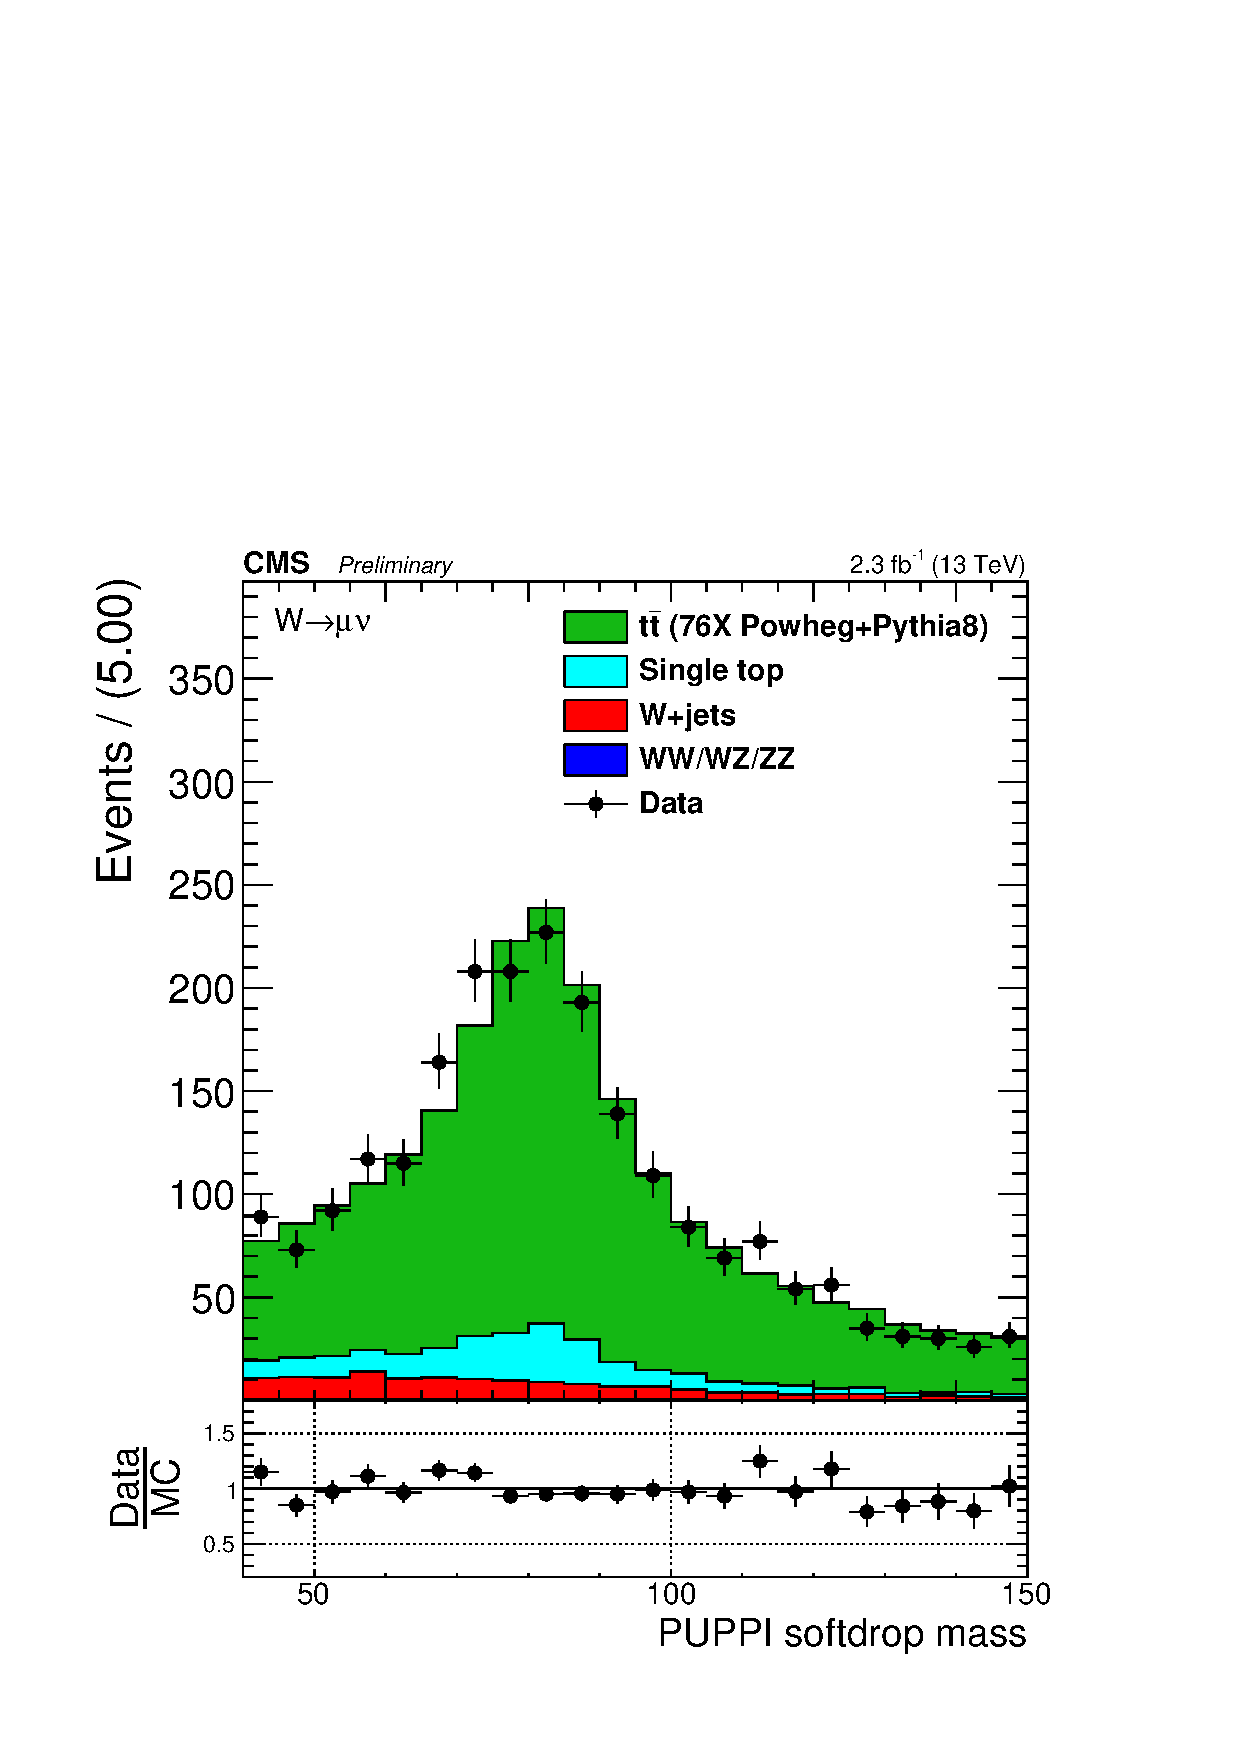
\includegraphics[width=0.5\textwidth]{figures/vtagging/AN-16-215/Whadr_puppi_softdrop_mu.pdf}
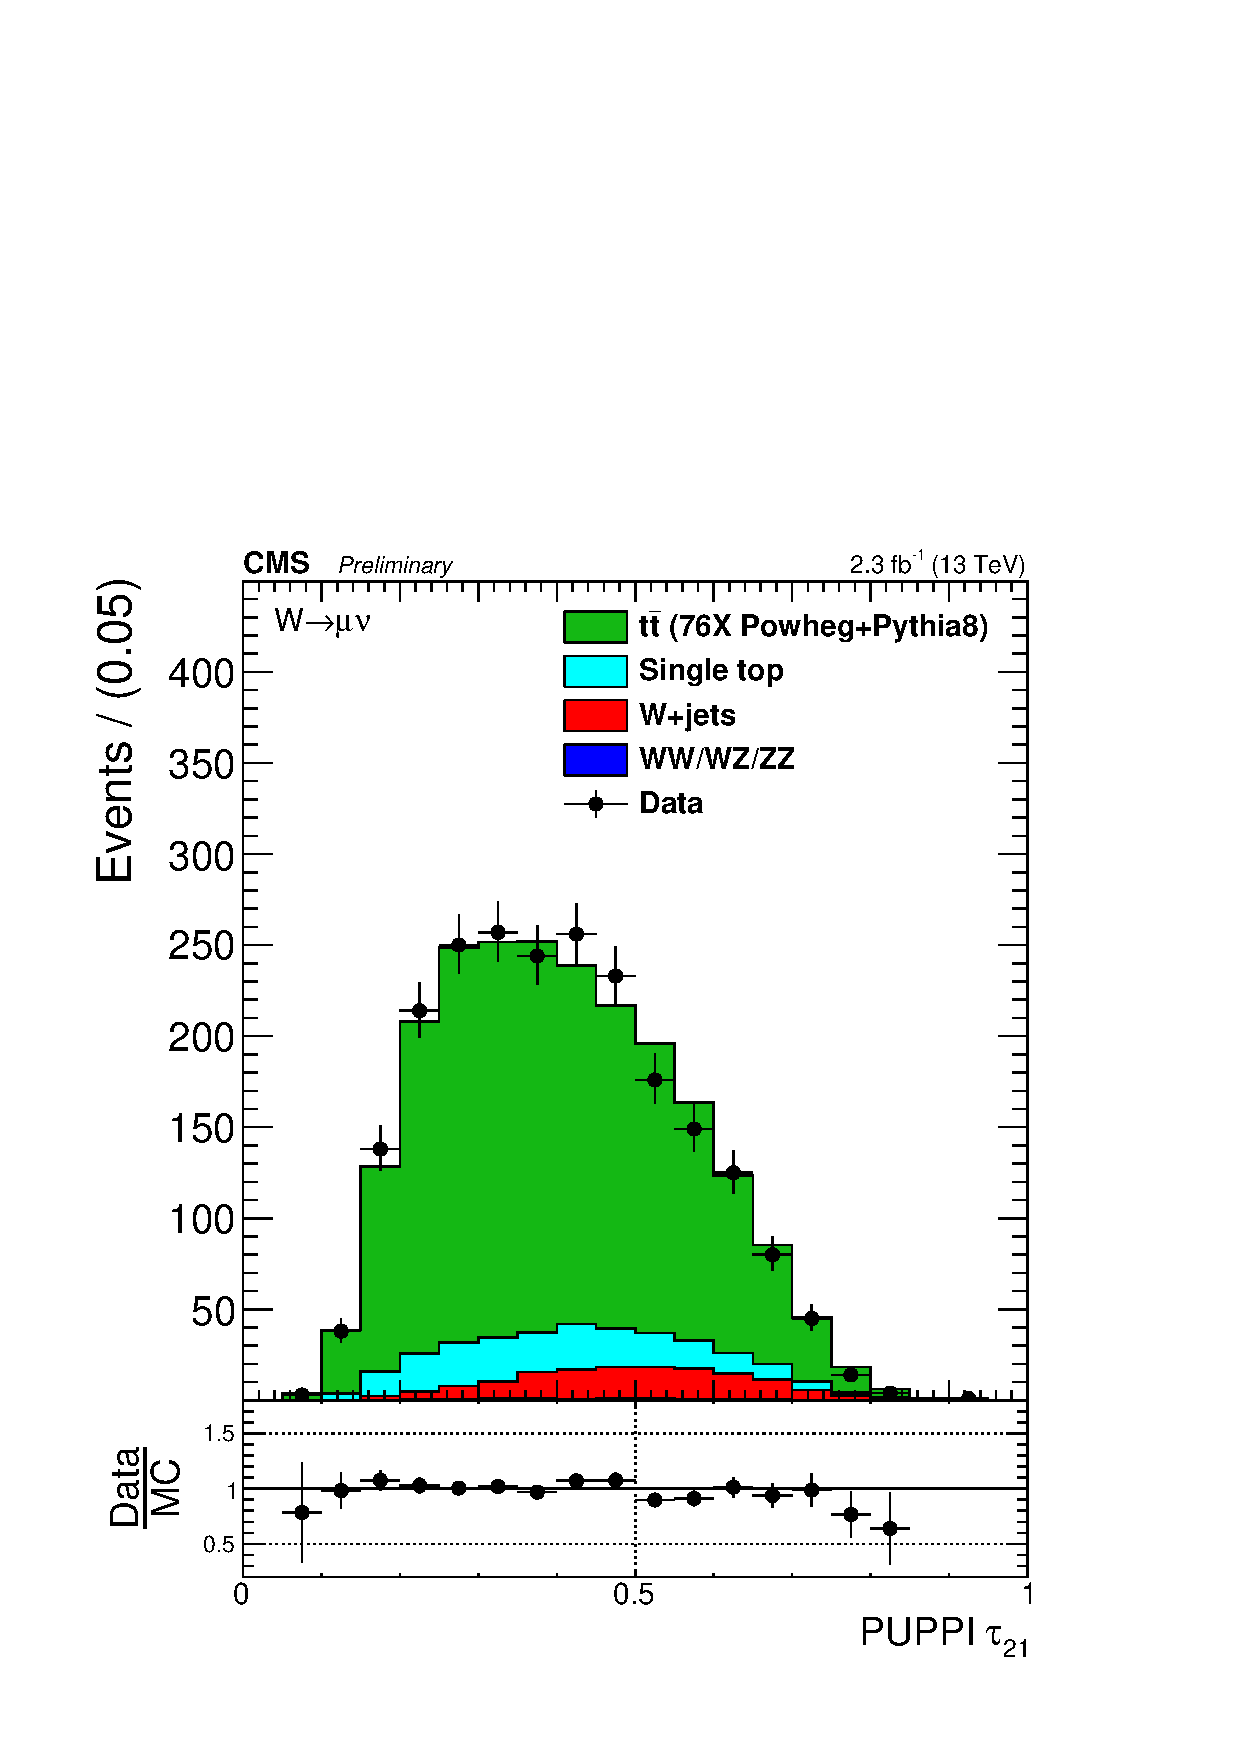
\includegraphics[width=0.5\textwidth]{figures/vtagging/AN-16-215/Whadr_puppi_tau2tau1_mu.pdf}\\
\end{tabular}
\caption{Distribution of the PUPPI softdrop mass (left) and PUPPI n-subjettiness (right) distribution in the \ttbar control sample.}
\label{fig:searchII:ttbarcp}
\end{figure}
%
% \paragraph{Fitting procedure:}
% For this measurement, what we are interested in is to extract and compare the W-tagging efficiency of the combined jet mass and \nsubj selection in data and in MC. We are additionally interested in the difference in jet mass scale (mean of the \PW jet mass peak) and jet mass resolution (width of \PW jet mass peak), as this also affects the signal jet mass shape and therefore efficiency. In order to study these variables, we look at the softdrop/pruned jet mass spectrum between 40 and 150 \GeV in two regions:
% \begin{itemize}
% \itemsep0em
%   \item Pass region: $0 <  \nsubj \leq 0.40$ for softdrop, $0 <  \nsubj \leq 0.45$ for pruning $\sim$ high purity
%   \item Fail region: $0.40 < \nsubj \leq 0.75$ for softdrop, $0.45 < \nsubj \leq 0.75$ for pruning  $\sim$ low purity
% \end{itemize}
% Our goal is to understand what the real fraction of merged \PW jets is in the pass category and in the fail category, assuming that the sum of the two correspond to a 100\% selection efficiency (the amount of \PW jets falling outside of this region is negligible).
% The strategy is the following: We first derive probability density functions (PDFs) which describe the distribution of fully merged \PW jets and non-\PW jets in \ttbar, both in the pass and in the fail region. The PDFs describing real \PW jets and non-\PW jets are added with a fraction which is left floating: the fit decides what the fraction of real \PW to non-\PW jets is in the pass and in the fail region. As simultaneous fit of pass and fail is then performed (using the two composite \PW+non-\PW PDFs), where the fraction of real \PW jets in both pass and fail is constrained such that, if the signal efficiency in pass is $\epsilon_S$, the signal efficiency in fail is ($1-\epsilon_S$). This is done by letting the normalization of the PDF describing real \PW jets in the pass category, be defined as the \textit{total} real \PW yield in pass and fail combined multiplied by some fraction, $\epsilon_S$. The normalization of the PDF describing real \PW jets in the fail category is then the total real \PW yield multiplied by ($1-\epsilon_S$).\newline
% To understand which part of the \ttbar jet mass distribution contains ``real'' merged Ws and which are only pure combinatorial background, non-PWs, we start from \ttbar MC.
% By matching the AK8 jet with quarks coming from the hadronic W at generator level, in a cone of $\Delta R < 0.8$, we can access the real merged \PW and non-merged \PW shapes.
% The real \PW and non-\PW PDFs for jets that pass and fail the N-subjettiness selection $\nsubj < 0.45$ or PUPPI $\nsubj < 0.4$, are found to be well described by the following functions:
% \begin{align*}
% f_{\rm bkg}(m_{j}) &= F_{\textrm{ExpErf}} = e^{c_0m_{j}} \cdot \frac{1 + {\rm Erf}((m_{j}-a)/b)}{2}  &\sim\textrm{for non-\PW jets in both pass and fail }\\
% f^{\rm sig}(m_{j}) &= F_{\rm Gaus}(m_{j}) + F_{\rm ExpErf}(m_{j})                                    &\sim\textrm{for real \PW jets in both pass and fail}
% \end{align*}
% Figure~\ref{fig:searchII:ttfitsd} shows the fitted PUPPI softdrop mass spectrum for \ttbar real \PW (top) and non-\PW (bottom) distributions for jets that passed (left) and failed (right column) the N-subjettiness selection PUPPI $\tau_{21}~<$~0.4.
% The corresponding plots for the jet pruned mass can be found in Figure~\ref{app:sf16}.
%
% \begin{figure}[htbp]
%   \centering
%     \includegraphics[width=0.49\textwidth]{figures/vtagging/AN-16-215/plots_76X/fits_TTMC/plots_em_HP0v40powheg_76X_PuppiSD_MCfits/{_TTbar_realWExoDiBosonAnalysis.WWTree_TTbar_powheg_76X_GausErfExp_ttbar_with_pull}.pdf}
%     \includegraphics[width=0.49\textwidth]{figures/vtagging/AN-16-215/plots_76X/fits_TTMC/plots_em_HP0v40powheg_76X_PuppiSD_MCfits/{_TTbar_realW_failtau2tau1cutExoDiBosonAnalysis.WWTree_TTbar_powheg_76X_GausErfExp_ttbar_failtau2tau1cut_with_pull}.pdf}\\
%     \includegraphics[width=0.49\textwidth]{figures/vtagging/AN-16-215/plots_76X/fits_TTMC/plots_em_HP0v40powheg_76X_PuppiSD_MCfits/{_TTbar_fakeWExoDiBosonAnalysis.WWTree_TTbar_powheg_76X_ErfExp_ttbar_with_pull}.pdf}
%     \includegraphics[width=0.49\textwidth]{figures/vtagging/AN-16-215/plots_76X/fits_TTMC/plots_em_HP0v40powheg_76X_PuppiSD_MCfits/{_TTbar_fakeW_failtau2tau1cutExoDiBosonAnalysis.WWTree_TTbar_powheg_76X_ErfExp_ttbar_failtau2tau1cut_with_pull}.pdf}
%   \caption{Fit to the real \PW (top) and non-\PW (bottom) softdrop jet mass distribution for jets that pass (left) and fail (right) the cut on PUPPI $\tau_{21}~<$~0.4.}
%   \label{fig:searchII:ttfitsd}
% \end{figure}
% These shapes constitute the fit functions used for the simultaneous fit. As can be seen from the fit to real \PW jets in the pass region, the distribution is not purely Gaussian and have a tail at higher groomed masses. This tail depends on the matching requirements used to define real merged \PW jets and is unphysical. We therefore assume that the distribution of real W-jets can be described by a Gaussian only, allowing the exponential error function  used to describe non W-jets to cover the contribution from the tails, hereby taking the number of real W-jets as the integral of the Gaussian shape only. This eliminates two additional fit functions, corresponding to six free parameters from the fit.
% In older estimations of the W-tagging scale factor based on the same procedure~\cite{CMS-PAS-B2G-16-021}), the functions used to describe the tail of the real W-jet distributions were also taken into account as contributing to the real W-jet tagging efficiency. These two calculations tests two extremes:
% The new method assumes a Gaussian peak, absorbing the tails into the background function making the fit more robust, while the old method assumes a Gaussian peak with tails estimated from matched MC. The latter uses a more precise definition of real \PW jets, but a less robust fit. Both methods were investigated and we found that the absorption of tails into the background function resulted in a decrease in the relative uncertainty on the final scale factor of 50 $\%$ and an overall improvement on the fit quality, reducing the fit $\chi^2$ by 15 $\%$. The fit parameters of the functions used to describe non W-jets in both the pass and in the fail region, are further constrained using the values obtained from matched \ttbar MC. The W-tagging scale factors ($SF_{HP}$), for the high purity selection ($\nsubj<0.45$/PUPPI $\nsubj<0.4$), are then extracted estimating the cut efficiency ($\epsilon_{HP}$) on both data and simulated samples fitting, simultaneously, pass and fail samples:
% \begin{align*}
% \footnotesize
%     L_{\rm pass} &= \prod_{i}^{N_{\rm evt}^{pass}} \bigg[N_{\rm W}\cdot\epsilon_{HP}\cdot f_{\rm pass}^{\rm sig}(m_{j}) + N_{\rm 2}\cdot f_{\rm pass}^{\rm bkg}(m_{j})+ \sum_{j=\textrm{ST,VV,WJet}} N^{j}_{\rm pass}\cdot f_{\rm pass}^{j}\bigg]\\
%     L_{\rm fail} &= \prod_{i}^{N_{\rm evt}^{fail}} \bigg[N_{\rm W}\cdot(1-\epsilon_{HP})\cdot f^{\rm sig}_{\rm fail}(m_{j}) + N_{\rm 3}\cdot f_{\rm fail}^{\rm bkg}(m_{j})+ \sum_{j=\textrm{ST,VV,WJet}} N^{j}_{\rm fail}\cdot f_{\rm fail}^{j}\bigg]
% \end{align*}
% where $N_{W}$ is the number of real W jets, $N_{2}$ and $N_{3}$ are the number of combinatorial background events passing and failing the \nsubj cut respectively. $N_{j}$ and $f_{j}$, with $j$ = ST, VV, WJet, are the normalizations and shapes of the minor backgrounds (single top, VV, W+jets) which are fixed from simulation. The fit functions used are
% \begin{alignat*}{3}
%     f_{\rm pass}^{\rm sTop} &= F_{\rm ErfExpGaus}(x) = &&\frac{1 + {\rm Erf}((x-a)/b)}{2} \cdot e^{-(x-x_{0})^{2}/2\sigma^{2}}\\
%     f_{\rm fail}^{\rm sTop} &= F_{\rm ExpGaus}(x)    = &&e^{ax} \cdot e^{-(x-b)^{2}/2s^{2}} && \quad \sim\rm{ Pruning}\\
%     f_{\rm fail}^{\rm sTop} &= F_{\rm ErfExpGaus}(x) = &&\frac{1 + {\rm Erf}((x-a)/b)}{2} \cdot e^{-(x-x_{0})^{2}/2\sigma^{2}} && \quad \sim \rm{ Softdrop}\\
%     f_{\rm pass}^{\rm VV}   &= F_{\rm ExpGaus}(x)    = &&e^{ax} \cdot e^{-(x-b)^{2}/2s^{2}}\\
%     f_{\rm fail}^{\rm VV}   &= F_{\rm ExpGaus}(x)    = &&e^{ax} \cdot e^{-(x-b)^{2}/2s^{2}}\\
%     f_{\rm pass}^{\rm wjet} &= F_{\rm ErfExp}(x)     = &&e^{c_0x} \cdot \frac{1 + {\rm Erf}((x-a)/b)}{2}\\
%     f_{\rm fail}^{\rm wjet} &= F_{\rm ErfExp}(x)     = &&e^{c_0x} \cdot \frac{1 + {\rm Erf}((x-a)/b)}{2}
% \end{alignat*}
% with the corresponding distributions shown in Figure~\ref{fig:searchII:minorbkrsd} for the PUPPI softdrop jet mass. The corresponding distributions for the pruned mass spectrum are can be found in Appendix~\ref{app:sf16}.
% \begin{figure}[h!]
%    \centering
%     \includegraphics[width=0.30\textwidth]{figures/vtagging/AN-16-215/{_STopExoDiBosonAnalysis.WWTree_STop_76X_ErfExpGaus_sp}.pdf}
%     \includegraphics[width=0.30\textwidth]{figures/vtagging/AN-16-215/{_WJets0ExoDiBosonAnalysis.WWTree_WJets_76X_ErfExp}.pdf}
%     \includegraphics[width=0.30\textwidth]{figures/vtagging/AN-16-215/{_VVExoDiBosonAnalysis.WWTree_VV_76X_ExpGaus}.pdf}\\
%     \includegraphics[width=0.30\textwidth]{figures/vtagging/AN-16-215/{_STop_failtau2tau1cutExoDiBosonAnalysis.WWTree_STop_76X_ErfExpGaus_sp}.pdf}
%     \includegraphics[width=0.30\textwidth]{figures/vtagging/AN-16-215/{_WJets0_failtau2tau1cutExoDiBosonAnalysis.WWTree_WJets_76X_ErfExp}.pdf}
%     \includegraphics[width=0.30\textwidth]{figures/vtagging/AN-16-215/{_VV_failtau2tau1cutExoDiBosonAnalysis.WWTree_VV_76X_ExpGaus}.pdf}
%   \caption{Fits to the PUPPI softdrop jet mass spectrum for the non-dominant backgrounds (Single top, W+jets and VV respectively) in the pass (top) and fail (bottom) regions.}
%   \label{fig:searchII:minorbkrsd}
% \end{figure}
% The floating parameters of the fit (besides the PDF shape parameters themselves) are the rates $N_{W}$, $N_{2}$ and $N_{3}$, and the mean and sigma of the W-mass distribution defined in
% $f^{\rm sig}_{\rm pass}(m_{j})$ and $f^{\rm sig}_{\rm fail}(m_{j})$. The ratio between data and simulation efficiencies are then taken as the W-tagging scale factor:
% \begin{equation}
%   \label{SF}
%   SF_{HP}= \frac{\epsilon_{HP}(\textrm{data})}{\epsilon_{HP}(\textrm{sim})}
% \end{equation}
% Considering that, both for data and simulation, $\epsilon_{HP}+\epsilon_{LP}+\epsilon_{fail} = 1$, the scale factor for low purity category can be defined as:
% \begin{equation*}
%   SF_{LP} = \frac{1-\epsilon_{HP}(\textrm{data})-\epsilon_{fail}(\textrm{data})}{1-\epsilon_{HP}(\textrm{sim})-\epsilon_{fail}(\textrm{sim})}
% \end{equation*}
% where $\epsilon_{fail}$ is the ratio between the number of events with $\tau_2/\tau_1 > 0.75$ and the total number of events. As mentioned previously, the number of real \PW jets with $\tau_2/\tau_1 > 0.75$  is negligible and the definition of the low purity scale factor simplifies to
% \begin{equation}
%   SF_{LP} = \frac{1-\epsilon_{HP}(\textrm{data})}{1-\epsilon_{HP}(\textrm{sim})}
% \end{equation}
%
% \paragraph{Systematic uncertainties:}
% As systematic uncertainties, we consider effects due to differences in \ttbar simulation as well as effects due to choice of fit method. The former is evaluated by comparing the extracted scale factor when using \ttbar MC samples produced with different matrix element (ME) and shower generators: \POWHEG (NLO) interfaced with \PYTHIA{8} , \MADGRAPH (LO) QCD interfaced with \HERWIG{++} and \POWHEG interfaced with \HERWIG{++}.
% The uncertainty due to different ME generators (\POWHEG versus \MADGRAPH correspond to 3-17\%, while the uncertainty due to parton showering (\PYTHIA{8} versus \HERWIG{++}) is 8.6\%. These are listed in Table~\ref{tab:WtagSFs}
% The uncertainty due to parton showering is not relevant for analyses where no \HERWIG{++} based simulation is used, as is the case for the search presented in this chapter.
% For the latter systematic uncertainty, accounting for effects due to choice of fit method, we compare the estimated extracted efficiency in \ttbar MC using the two different fit models described above: The new model, where the signal is modeled by a Gaussian peak and the tails of the distribution are absorbed in the background fit model, and the old model, including the tails when calculating the fraction of real \PW jets. Figure~\ref{fig:searchII:gausvstails} shows the fits obtained in the pass and fail regions using the two different models. With the new model only the Gaussian component of the fit contributes to the W-tagging efficiency while, with the old model, a Chebyshev component is additionally contributing to the total W-tagging efficiency.
% \begin{figure}[ht!]
%   \centering
%     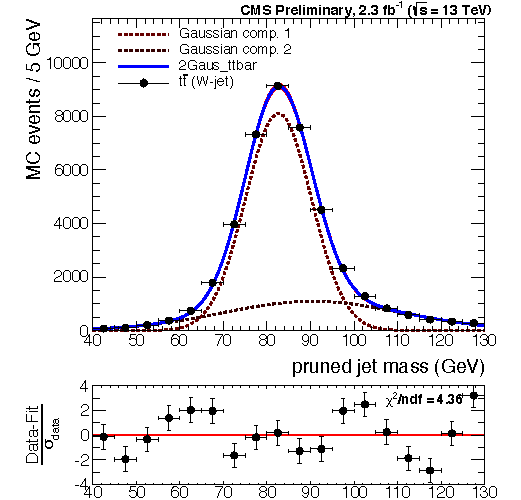
\includegraphics[width=0.49\textwidth]{figures/vtagging/AN-16-215/2Gauss.pdf}
%     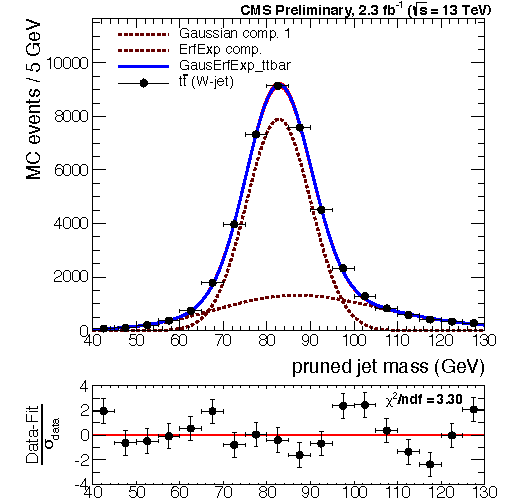
\includegraphics[width=0.49\textwidth]{figures/vtagging/AN-16-215/GausErfExpPass.pdf}\\
%     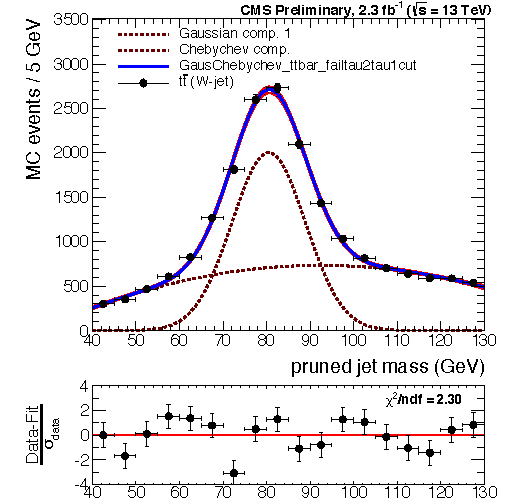
\includegraphics[width=0.49\textwidth]{figures/vtagging/AN-16-215/GausChebysgev.pdf}
%     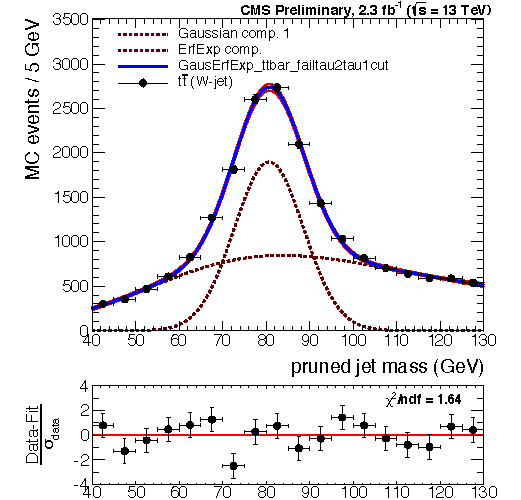
\includegraphics[width=0.49\textwidth]{figures/vtagging/AN-16-215/GausErfExpFail.pdf}
%   \caption{Fits obtained in the pass (top) and fail (bottom) regions using two different models: An alternative model with tails (top and bottom, left) where the tail component is contributing to the total W-tagging efficiency. When using the default model (top and bottom, right), only the Gaussian component of the fit contributes to the W-tagging efficiency.}
%   \label{fig:searchII:gausvstails}
% \end{figure}
% The estimated efficiencies obtained using both methods, after being corrected for the fraction of \PW jets in the tails, agree within 0.3-12\% and are listed as systematic uncertainty in Table~\ref{tab:WtagSFs}.\newline
% One additional uncertainty is added. As the W-tagging scale factor is evaluated in a \ttbar sample, the transverse momentum range is rather limited. When the \PW \PT reaches $\sim 400 \GeV$, the AK8 jet becomes a fully merged top jet with a mass of 170 \GeV and a scale factor measurement becomes impossible. However, the jets used in the analyses presented in this thesis have very high transverse momenta, up to 2-3 \TeV, and we therefore need an estimate of how the uncertainty on the W-tagging scalefactor changes as a function of \PT. This is estimated by comparing the difference in tagging between $\BulkG \rightarrow \PW \PW$ signal MC showered by \PYTHIA{}8 and \HERWIG{++} as a function of \PT, relative to the difference in tagging efficiency between the two at a $\PT \sim 200$~\GeV. This measurement was performed by a separate analysis team, and found to be $5.90\% \times \ln(\pt/200\GeV)$.
%
% % \begin{figure}[htbp]
% %   \centering
% %     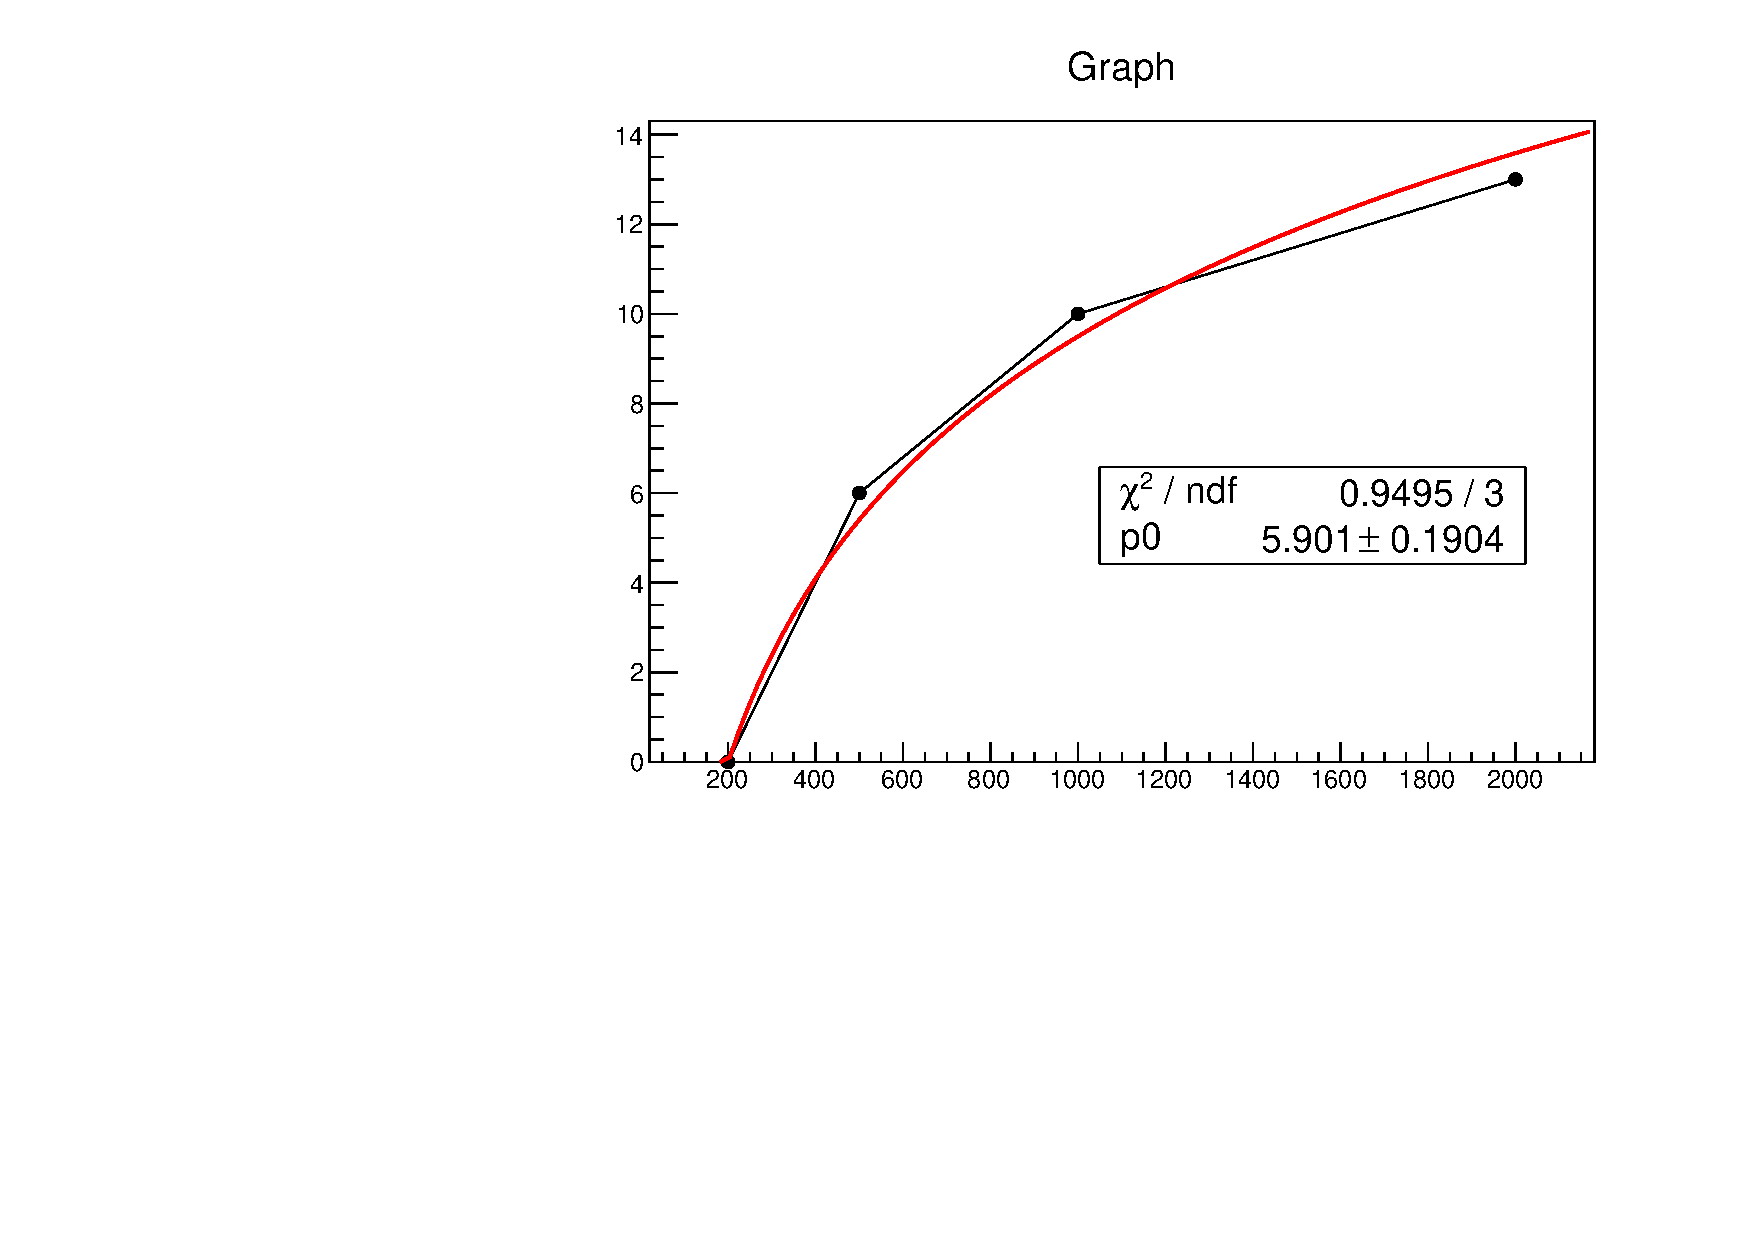
\includegraphics[width=0.50\textwidth]{figures/vtagging/AN-16-215/wtag-ptdependence-tau21tight.pdf}
% %   \caption{Uncertainty on the \pt dependence of the scale factor as a function of \pt, approximated with a logarithmic function.}
% %   \label{fig:ptdependence}
% % \end{figure}
%
% Systematic uncertainties from other sources (lepton identification, b tagging etc.) are less than 0.5\% and therefore negligible.
%
% \paragraph{Results:}
% The simultaneous fit as described above is then performed both for data and for simulation, where we take the ratio of data and MC efficiencies as efficiency scale factors.
% The corresponding fits are shown in Figure~\ref{fig:searchII:simfit}, with the corresponding extracted efficiencies and scale factors summarized in Table~\ref{tab:WtagSFs}.
%
% \begin{table}[h!]
%    \centering
%    \begin{tabular}{lll}
%    \hline
%    Category & Working point & Eff. data & Eff. simulation & Scale factor\\
%    \hline
%    High-purity Pruning & ($\tau_2 / \tau_1 < 0.45$)                   & $0.775 \pm 0.041 $& $0.822 \pm 0.033$                     &$0.94 \pm 0.05~\rm{(stat)} \pm 0.03~\rm{(sys)} \pm 0.003~\rm{(sys)}$\\
%    Low-purity Pruning & ($0.45 < \tau_2 / \tau_1 < 0.75$)             & $0.225 \pm 0.041 $& $0.178 \pm 0.033$                     &$1.27 \pm 0.25~\rm{(stat)} \pm 0.13~\rm{(sys)} \pm 0.008~\rm{(sys)}$\\
%    \hline
%    High-purity PUPPI softdrop & ($\tau_2 / \tau_1 < 0.4$)             & $0.785 \pm 0.045 $& $0.81 \pm 0.01$\\                     &$0.97 \pm 0.06~\rm{(stat)} \pm 0.04~\rm{(sys)} \pm 0.06~\rm{(sys)}$\\
%    Low-purity PUPPI softdrop & ($0.45 < \tau_2 / \tau_1 < 0.75$)      & $0.215 \pm 0.057 $& $0.204 \pm 0.041$                     &$1.13 \pm 0.24~\rm{(stat)} \pm 0.17~\rm{(sys)}  \pm 0.12~\rm{(sys)}$\\
%    \end{tabular}
%    \label{tab:WtagSFs}
%    \caption{W-tagging scale factors for both categories the high purity and low purity categories for two taggers: Pruned jet mass + \nsubj and PUPPI softdrop jet mass + PUPPI \nsubj. }
% \end{table}
%
%
% \begin{figure}[htbp]
% \centering
% \includegraphics[width=0.44\textwidth]{figures/vtagging/AN-16-215/_HP0v45powheg_76X_em_pTbin_200_5000.pdf}
% \includegraphics[width=0.44\textwidth]{figures/vtagging/AN-16-215/_HP0v45powheg_76X_em_fail_pTbin_200_5000.pdf} \\
% \includegraphics[width=0.44\textwidth]{figures/vtagging/AN-16-215/_HP0v40powheg_76X_PuppiSD_em_pTbin_200_5000.pdf}
% \includegraphics[width=0.44\textwidth]{figures/vtagging/AN-16-215/_HP0v40powheg_76X_PuppiSD_em_fail_pTbin_200_5000.pdf}\\
% \caption{Pruned jet mass distribution that pass (left) and fail (right) the $\tau_2 / \tau_1 < 0.45$ (top) and PUPPI $\tau_2 / \tau_1 < 0.40$ selection (bottom). Results of both the fit to data (blue) and simulation(red) are shown. The background components of the fit are shown as short-dashed lines.}
% \label{fig:searchII:simfit}
% \end{figure}
%
% We additionally subtract the jet mass scale and jet mass resolution, u
% To extract corrections to the jet mass scale and resolution, we use the
% mean $\langle m \rangle$ and resolution $\sigma$ value of the Gaussian
% component of the fitted function of the W bosons in the passed
% sample.
% The fits are shown for the
% $\tau_2 / \tau_1 < 0.45$ selection in Fig.~\ref{fig:ttbarControl_nocut} (a) and for the
% PUPPI $\tau_2 / \tau_1 < 0.40$ selection in Fig.~\ref{fig:ttbarControl_nocut} (c), and the
% resulting parameters are summarized in Table~\ref{tab:params}.  We find
% that both the W jet mass scale and resolution in data are larger than
% that in simulation.
%
% \begin{table}[!htb]
%  \begin{center}
% \caption{Summary of the fitted W-mass peak fit parameters.}
% \label{tab:params}
%  \begin{tabular}{c|c|c|c}
%   Parameter & Data & Simulation & Data/Simulation \\
%   \hline
%   Pruning $\langle m \rangle$ &$80.9 \pm 0.6~{\rm \GeV}$ & $82.5 \pm 0.1~{\rm \GeV}$ & $0.980 \pm 0.007$ \\
%   Pruning $\sigma$ & \ $6.7 \pm 0.7~{\rm \GeV}$ & \ $7.5 \pm 0.3~{\rm \GeV}$ & $0.89 \pm 0.10$ \\
%   \hline
%   % PUPPI softdrop $\langle m \rangle$ &$86.8 \pm 0.8~{\rm \GeV}$ & $87.9 \pm 0.2~{\rm \GeV}$ & $0.988 \pm 0.010$ \\
% %   PUPPI softdrop $\sigma$ & \ $9.2 \pm 1.0~{\rm \GeV}$ & \ $8.7 \pm 0.4~{\rm \GeV}$ & $1.07 \pm 0.09$ \\
%   PUPPI softdrop $\langle m \rangle$ &$80.3 \pm 0.8~{\rm \GeV}$ & $81.9 \pm 0.01~{\rm \GeV}$ & $0.98 \pm 0.01$ \\%New mass corrections
%   PUPPI softdrop $\sigma$ & \ $9.0 \pm 0.9~{\rm \GeV}$ & \ $8.5 \pm 0.4~{\rm \GeV}$ & $1.07 \pm 0.12$ \\%New mass corrections
%  \end{tabular}
%  \end{center}
% \end{table}
%
%
%
%
%  % \begin{figure}[htbp]
% %  \centering
% %  \begin{tabular}{cc}
% %  \includegraphics[width=0.45\textwidth]{figures/vtagging/AN-16-215/plots_76X/plots_0v45/model_data_em.pdf}
% %  \includegraphics[width=0.45\textwidth]{figures/vtagging/AN-16-215/plots_76X/plots_0v45/model_TotalMC_em.pdf}\\
% %  \includegraphics[width=0.45\textwidth]{figures/vtagging/AN-16-215/plots_76X/plots_0v45/model_data_failtau2tau1cut_em.pdf}
% %  \includegraphics[width=0.45\textwidth]{figures/vtagging/AN-16-215/plots_76X/plots_0v45/model_TotalMC_failtau2tau1cut_em.pdf}\\
% %  \end{tabular}
% %  \caption{Fit results in data (left) and simulation (right) after simultaneous fit.
% % Top: pass selection($\tau_{21} < 0.45$), bottom: fail selection($\tau_{21} > 0.45$). }
% %  \label{fig:Wtagging_sf_045}
% %  \end{figure}
% %
% %   \begin{figure}[htbp]
% %   \centering
% %   \begin{tabular}{cc}
% %   \includegraphics[width=0.45\textwidth]{figures/vtagging/AN-16-215/model_data_em.pdf}
% %   \includegraphics[width=0.45\textwidth]{figures/vtagging/AN-16-215/model_TotalMC_em.pdf}\\
% %   \includegraphics[width=0.45\textwidth]{figures/vtagging/AN-16-215/model_data_failtau2tau1cut_em.pdf}
% %   \includegraphics[width=0.45\textwidth]{figures/vtagging/AN-16-215/model_TotalMC_failtau2tau1cut_em.pdf}\\
% %   \end{tabular}
% %   \caption{Fit results in data (left) and simulation (right) after simultaneous fit.
% %  Top: pass selection(PUPPI $\tau_{21} < 0.40$), bottom: fail selection(PUPPI $\tau_{21} > 0.40$). }
% %   \label{fig:Wtagging_sf_040}
% %   \end{figure}
%

\subsection{W-tagging mistagging rate measurement} 

We additionally measure the W-tagging fake rate in data in a QCD dijet enriched region and compare this to the prediction from QCD MC using the three different combination of generators described above (\HERWIG{++}, \PYTHIA and \MADGRAPH+\PYTHIA).
Figure~\ref{fig:searchII:fakerate} shows the mistag rate as a function of \PT

\begin{figure}[htbp]
\centering
\includegraphics[width=0.49\textwidth]{figures/vtagging/JME-16-003/BoostedW/BkgEff_DataMC_herwig_pT.pdf}
\includegraphics[width=0.49\textwidth]{figures/vtagging/JME-16-003/BoostedW/BkgEff_DataMC_Pythia8_pT.pdf}\\
\includegraphics[width=0.49\textwidth]{figures/vtagging/JME-16-003/BoostedW/BkgEff_DataMC_Pythia8Madgraph_pT.pdf}
\caption{ 
Fraction of jets passing the $m_{\mathrm{jet}}$ and $\tau_2/\tau_1$ selections in a dijet data sample and in
simulation as a function of \pt, comparing (a) \HERWIG{++}, (b) \PYTHIA{8} and (c) \PYTHIA{8} with \MADGRAPH as matrix-element generator.
The data over simulation ratio is shown for the combination of the $m_{\mathrm{jet}}$ and $\tau_2/\tau_1$ selections.}
\label{fig:searchII:fakerate}
\end{figure}

\subsection{Efficiency scale factors for 12.9 and 35.9 \fbinv} 
\label{sec:searchII:wtagsfana}
\section{Results for the full 2016 dataset}   
\label{sec:searchII:brg17001res}

